\chapter{State of The Art} \label{chap:stateOfTheArt}
%\begin{flushright}{\slshape    
%   Science, my boy, is made up of mistakes, but they are mistakes
%   which it is useful to make, because they lead little by little
%   to the truth}. \\ \medskip --- \citeauthor{verne_journey:1957}
%   \citetitle{verne_journey:1957} \citeyear{verne_journey:1957}
%\end{flushright} 

\lettrine[lines=4]{\textcolor{purple}{T}}{his} chapter contains an overview of the highest level of developments in the information technology fields 
which represent a solid foundation for the development of this thesis.
%\lettrine[lines=4]{\textcolor{purple}{T}}{he} term "big data" refers to a  research branch that deals with methodologies to analyze and extract information from data sets containing data that can be structured, as in the traditional relational databases, semi-structured, like the self-described XML or JSON documents, or unstructured, as the logfiles collected mostly by web applications to monitor usage or other user's preferences. More properly, we call big data those that cannot be handled using traditional database and software technologies. 
%Today, every second 8,411 Tweets are sent, 902 Instagram photos are uploaded, 1,502 Tumblr posts are created, 3,690 Skype calls are done, 73,116 Google searches are performed and 2,780,000 emails are sent\footnote{Data source: \url{http://www.internetlivestats.com/}}~\cite{misc:InternetLiveStats}. 
\section{Big Data}\label{sec:big_data}
The term "big data" refers to a  research branch that deals with methodologies to analyze and extract information from data sets containing data that can be structured, as in the traditional relational databases, semi-structured, like the self-described XML or JSON documents, or unstructured, as the logfiles collected mostly by web applications to monitor usage or other user's preferences. More properly, we call big data those that cannot be handled using traditional database and software technologies. 
IDC~\cite{misc:IDC} has predicted that by 2020 one tenth of the world’s data will be produced by machines. The organisation forecast that in five years time the amount of connected devices communicating over the internet will reach 32 billion and generate 10\% of the world’s data.
This data is collected and analyzed. 
%Gartner's definition of big data is: "Big data is high-volume, high-velocity and/or high-variety information assets that demand cost-effective, innovative forms of information processing that enable enhanced insight, decision making, and process automation"\footnote{\url{https://www.gartner.com/it-glossary/big-data/}}. This defintion relates to something known as the three V's characterizing big data: Volume, Velocity,Variety~\cite{WhatIsBigData}. Volume is important because the amount of data matters. With big data, you’ll have to process high volumes of low-density, unstructured data. This can be data of unknown value, such as Twitter data feeds, clickstreams on a webpage or a mobile app, or sensor-enabled equipment. For some organizations, this might be tens of terabytes of data. For others, it may be hundreds of petabytes. Velocity is the fast rate at which data is received and (perhaps) acted on. Normally, the highest velocity of data streams directly into memory versus being written to disk. Some internet-enabled smart products operate in real time or near real time and will require real-time evaluation and action. Variety refers to the many types of data that are available. Traditional data types were structured and fit neatly in a relational database. With the rise of big data, data comes in new unstructured data types. Unstructured and semistructured data types, such as text, audio, and video require additional preprocessing to derive meaning and support metadata. By means of hardware virtualization, cloud computing services satisfies all the requested requisites needed to manipulate big data. Elasticity and redundancy provided by cloud computing also enable big data application high availability, scalability and fault tolerance.
%Big data also is an unprecedented business opportunity for many companies which  deliver big data applications as a service. According to  SoftwareTestingHelp~\cite{misc:BigDataCompanies}, these are the top 10 big data companies of 2019: IBM~\cite{misc:IBM}, HP Enterprise~\cite{misc:HPE}, Teradata~\cite{misc:Teradata}, Oracle~\cite{misc:Oracle}, SAP~\cite{misc:SAP}, Dell EMC~\cite{misc:EMC}, Amazon~\cite{misc:AWS}, Microsoft~\cite{misc:Microsoft}, Google~\cite{misc:Google}, VMware~\cite{misc:VMware}.

\subsection{Batch Processing: Hadoop}\label{sec:map_reduce_hadoop}
%\section{Hadoop}\label{sec:hadoop}
Hadoop~\cite{misc:ApacheHadoop} uses the Map-Reduce programming model that was firstly introduced by Google~\cite{misc:GoogleMapReduce} and consists of two distinct phases: Map and Reduce.
%MapReduce is a software framework firstly introduced by Google in order to support the distributed computation of large dataset in cluster of computers. The framework is inspired by map and reduce functions used in functional programming, even though their purpose in the MapReduce framework is not the same as in the original form.

The former processes and \textit{transforms} a block of data to produce key-value pairs (tuples) as intermediate outputs, the latter \textit{aggregates} these tuples into a final output.
There are available MapReduce libraries written in different programming languages. 
\begin{figure}
	\vspace{-1.7cm}
	\centering
	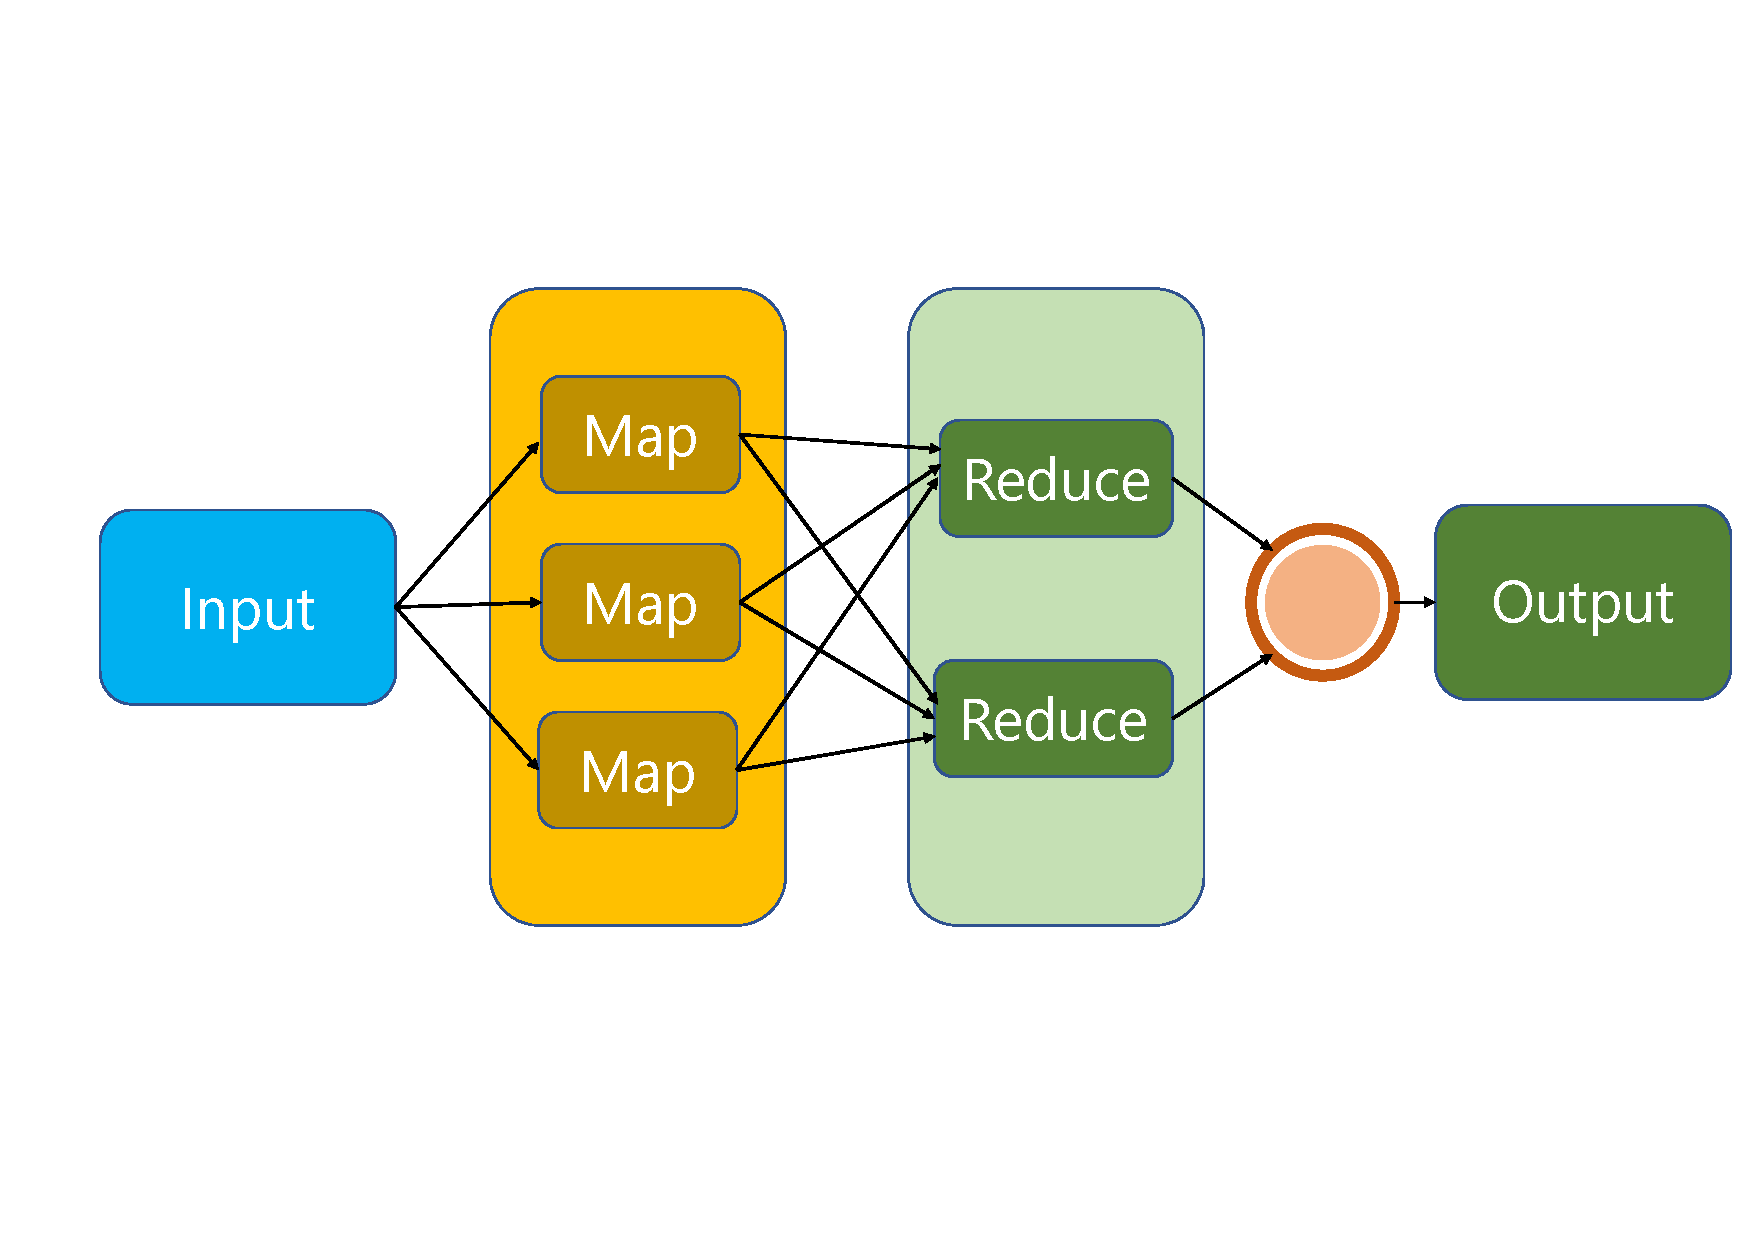
\includegraphics[width=\columnwidth]{Images/map_reduce_1.pdf}  
	\vspace{-2cm}
	\caption[map-reduce model]{Abstract representation of map-reduce paradigm}
	\vspace{0.5cm}
	\label{fig:mapReduce}
\end{figure}

MapReduce is a programming framework that allows us to perform distributed and parallel processing on large data sets in a distributed environment.\footnote{Extracted from: \url{https://www.edureka.co/blog/mapreduce-tutorial/}}.
\begin{itemize}
	\item MapReduce consists of two distinct tasks – Map and Reduce.
	\item As the name MapReduce suggests, reducer phase takes place after mapper phase has been completed.
	\item So, the first is the map job, where a block of data is read and processed to produce key-value pairs as intermediate outputs.
	\item The output of a Mapper or map job (key-value pairs) is input to the Reducer.
	\item The reducer receives the key-value pair from multiple map jobs.
	\item Then, the reducer aggregates those intermediate data tuples (intermediate key-value pair) into a smaller set of tuples or key-value pairs which is the final output.
\end{itemize}

Open source implementation of the MapReduce framework, include Apache Hadoop~\cite{misc:ApacheHadoop}. 
The MapReduce framework is composed by the following functions:
\begin{enumerate}
	\item Input Reader
	\item Map Function
	\item Partition Function
	\item Compare Function
	\item Reduce Function
	\item Output Writer
\end{enumerate}

The Input Reader reads data from mass storage and splits it in many different fragments of fixed size (e.g., 128 MB) and then it distributes them to the servers of the cluster hosting the Map function. It also generates a (key, value) pair. One of the servers of the cluster is elected to be the master, and is in charge of detecting idle slaves and assign them a task, and the others are slaves that are assigned tasks by the master. Each slave running a task reads the content of the input, extracts the (key, value) pairs and send them to the user-defined Map function, that generates (key, value) pairs as output, that are stored in memory and periodically cached on disk. They are also partitioned in sections by the partition function. The addresses of the partitioned sections are sent to the master node which is responsible of rotating the location of the slaves that process the Reduce function. All the pairs are reordered while transitioning between the slave with the Map function and the slave with the Reduce function, in order to group pairs with the same key on the same server. This is the shuffling phase. 

Once all the keys that point to the same value are discovered using the compare function, a merge is done. Sorting is useful so that the reducer knows when a new reduce task should start. For each key, the Reduce function defined by the user is applied to the values having the same key, generating one or more ouput element. The Output Writer writes the results to mass storage.
\begin{figure}
	\vspace{-1cm}
	\centering
	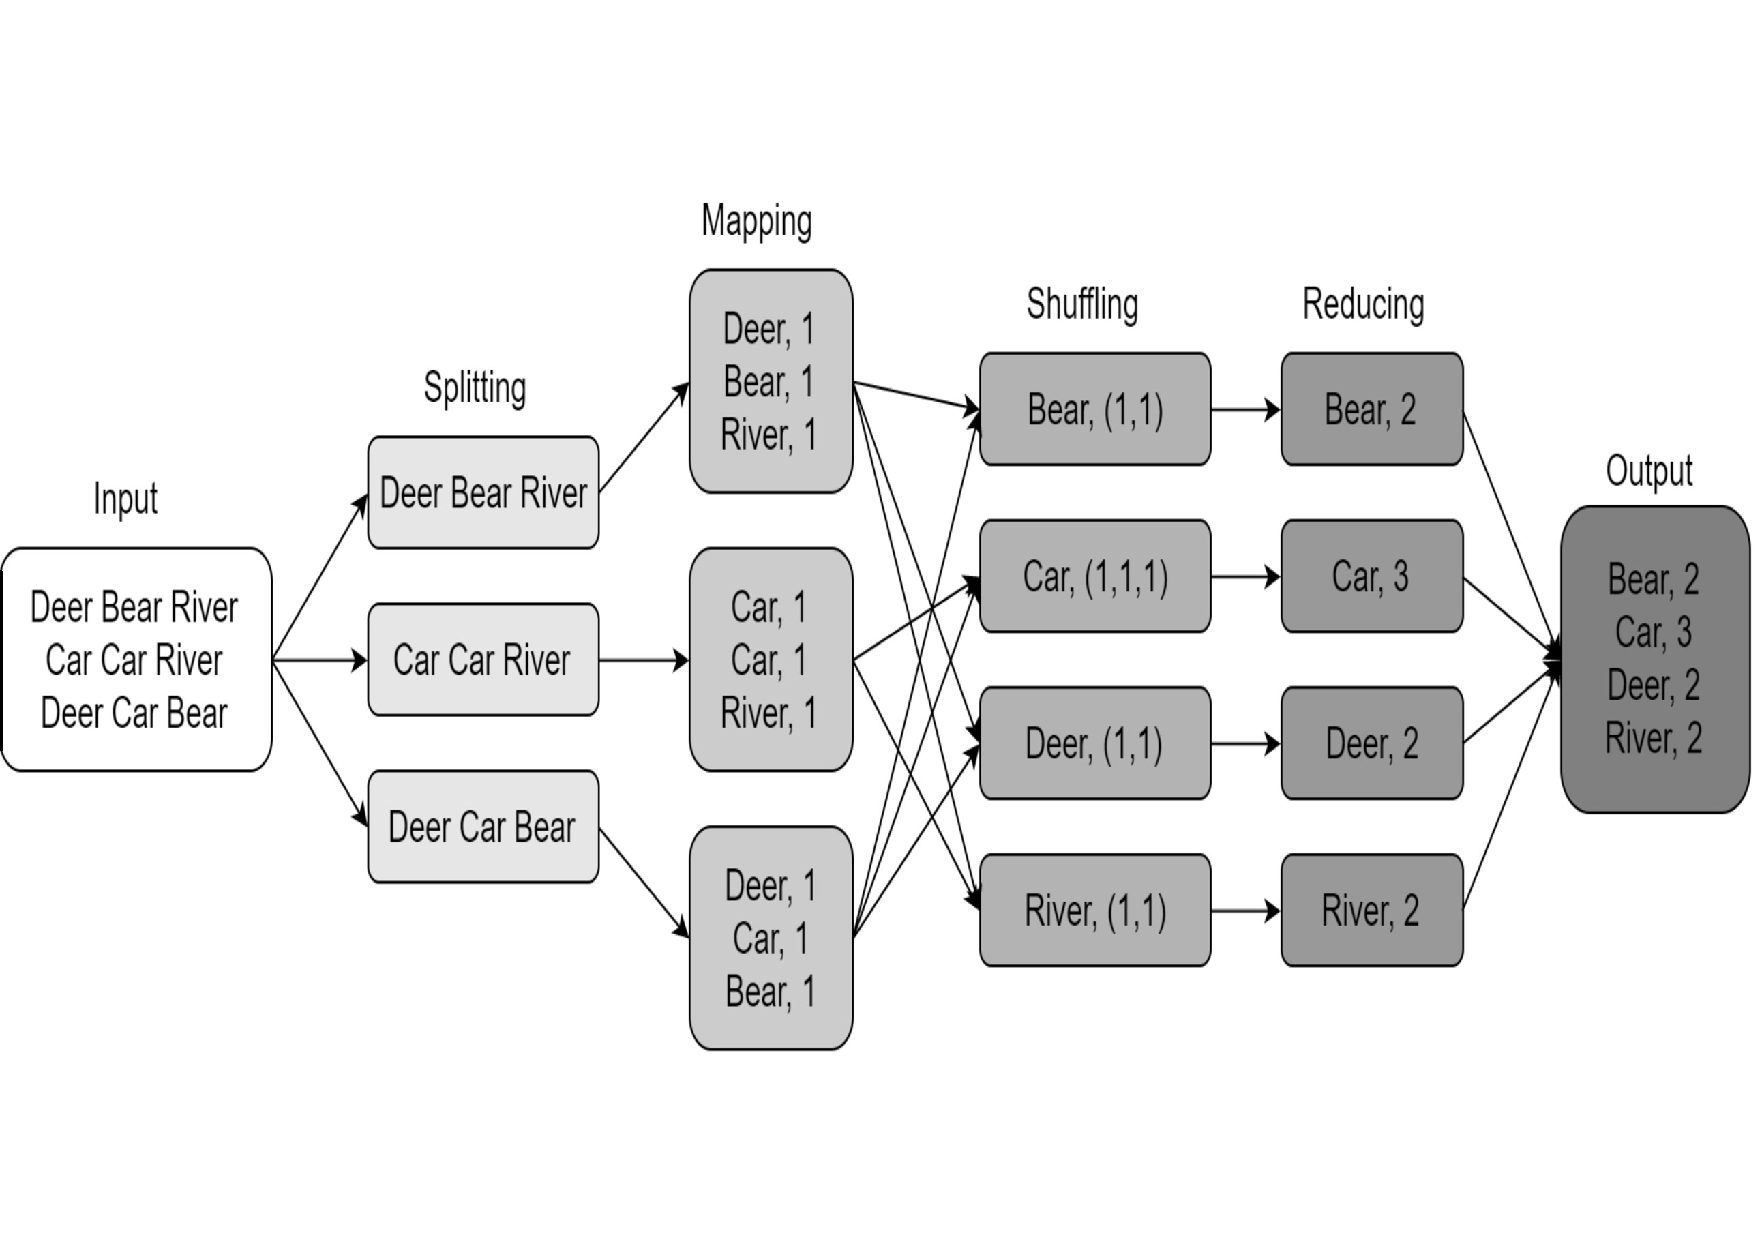
\includegraphics[width=\columnwidth]{Images/word_count_example.pdf}  
	\vspace{-1.5cm}
	\caption[map-reduce model]{Map-Reduce word count job example. Counts the occurrence of each word in input}
	\label{fig:wordCountExample}
\end{figure}

A sample word count application is shown in \myFig{fig:wordCountExample} The input is a document containing words, and we have to compute the cardinality of the occurrence of each word in the document. Each Map task is applied to a line of the document, producing pair (’word’, 1) for each word. For example if the input line is "Dear Bear River", it is split into ["Dear", "Bear", "River"] and then mapped into [("Dear", 1), ("Bear", 1), ("River", 1)]. After shuffling the results of the Map, the Reduce task receives a word and a list containing as many ones as the cardinality of the word occurrence in the document. The Reduce function will sum the ones in the list and producing as a result the pair (’word’, ’count’). For example, a reducer can receive the key "Bear" with list of values (1, 1), this is reduced into ("Bear", 2). Reducers results are then collected and storedto disk.

%Apache Hadoop\footnote{url: https://hadoop.apache.org/docs/} is an open-source framework for distributed storage and processing of big data sets using MapReduce programming model.

\begin{figure}
	\vspace{-1cm}
	\centering
	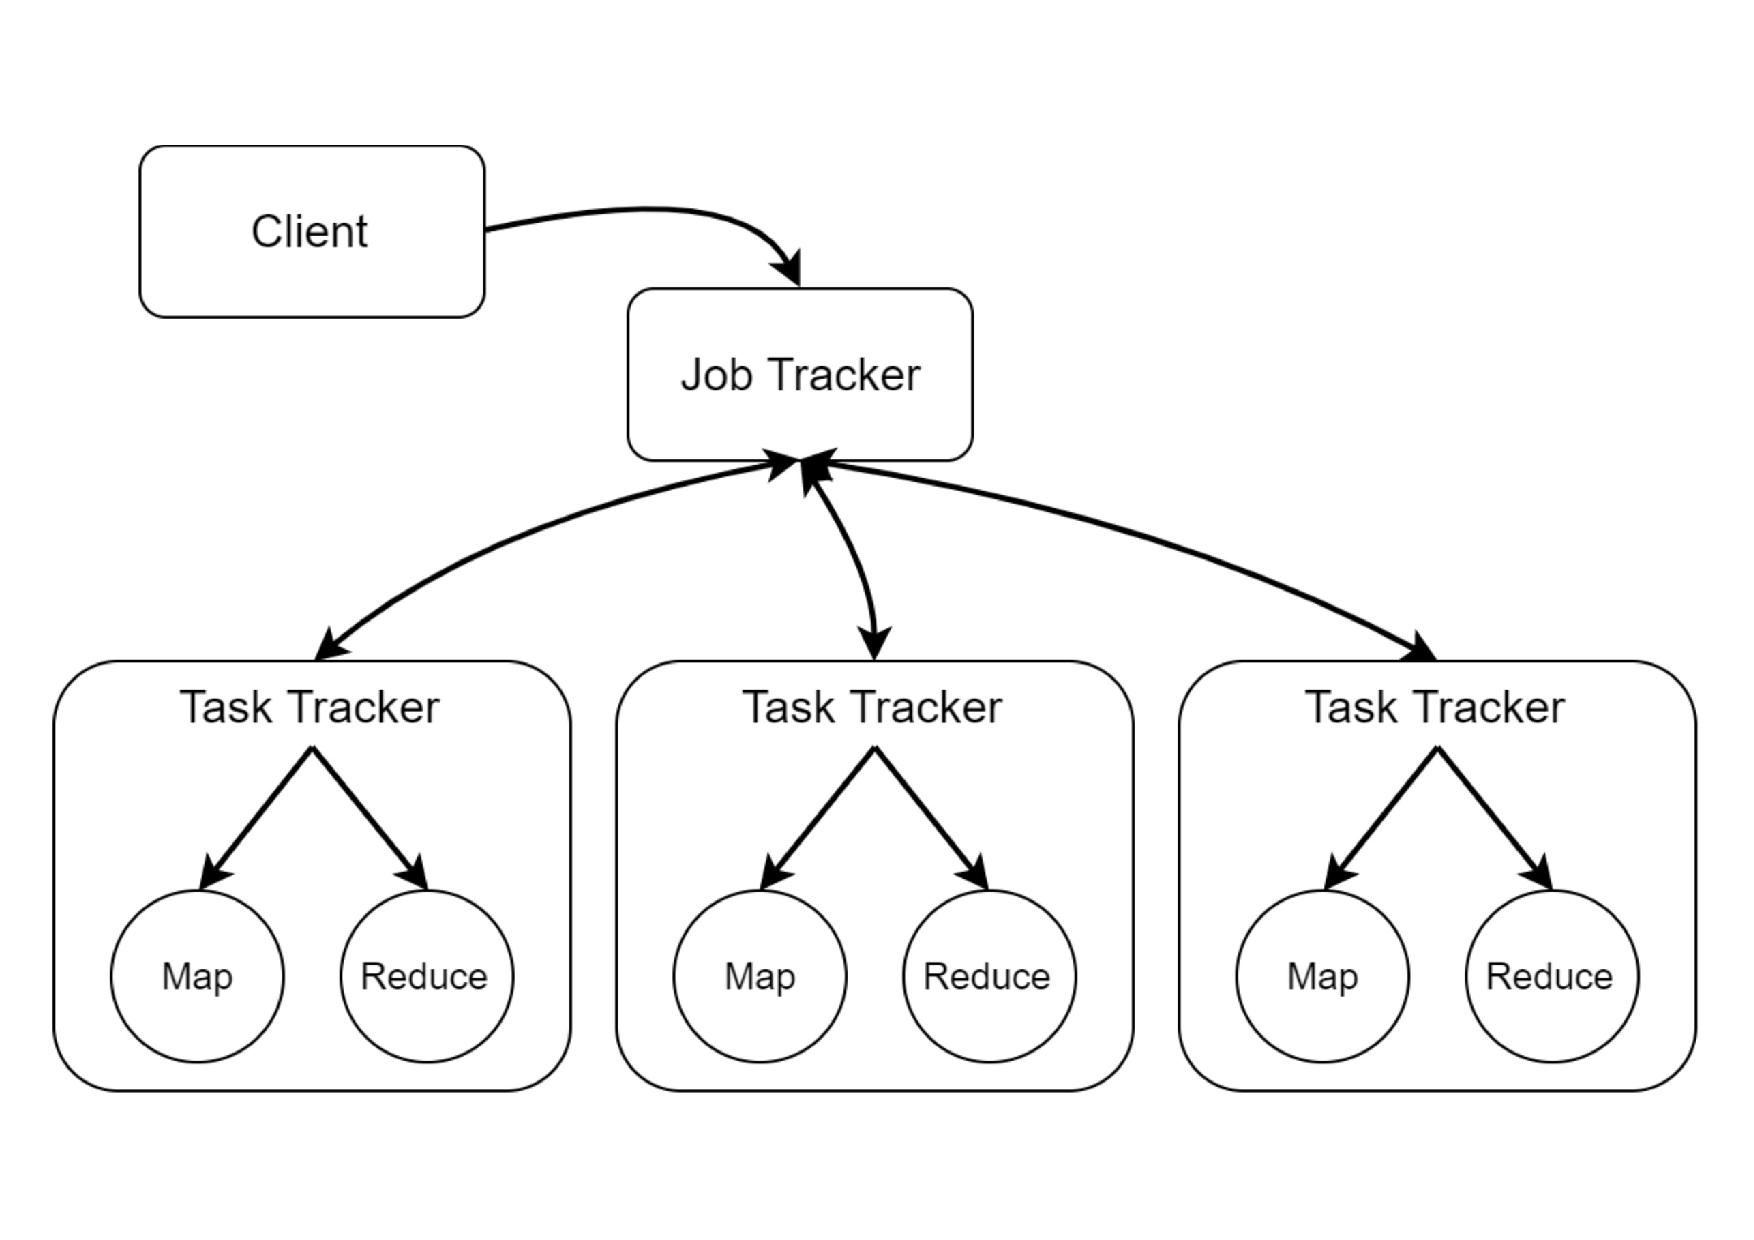
\includegraphics[width=\columnwidth]{Images/hadoop_map_reduce_architecture.pdf}  
	\vspace{-1cm}
	\caption[hadoop map-reduce architecture]{Hadoop Map-Reduce Architecture.}
	\label{fig:hadoopMapReduceArchitecture}
\end{figure}

Apache Hadoop MapReduce cluster has a centralized structure composed by a master Job Tracker (JT) and multiple worker nodes running Task Tracker (TT), as shown in  \myFig{fig:hadoopMapReduceArchitecture}. 

JT organizes the job tasks on the slave nodes and continuously polls the Task Trackers by means of heartbeats. Heartbeats retrieve information about the liveliness of the slaves and to inspect the progress of the task  executions. If a task execution fails, it is re-executed possibly on a different slave. JT is also the cluster manager, so it check the eligibility of the submitted MapReduce jobs. TT runs the assigned task and replies to heartbeats in order to affirm their liveliness and update the master about the progress of the assigned tasks. %They are configured with a fixed number of map and reduce task slots.

Apache Hadoop also offers a distributed filesystem that stores data on several machine, providing a high aggregate bandwidth across the cluster. It is called Hadoop Distributed File System (HDFS)\footnote{\textit{HDFS Architecture Guide.} \url{https://hadoop.apache.org/docs/r1.2.1/hdfs\_design.html}}. 
It is highly fault tolerant and designed to run on commodity hardware.
\begin{figure}
	\vspace{-1.5cm}
	\centering
	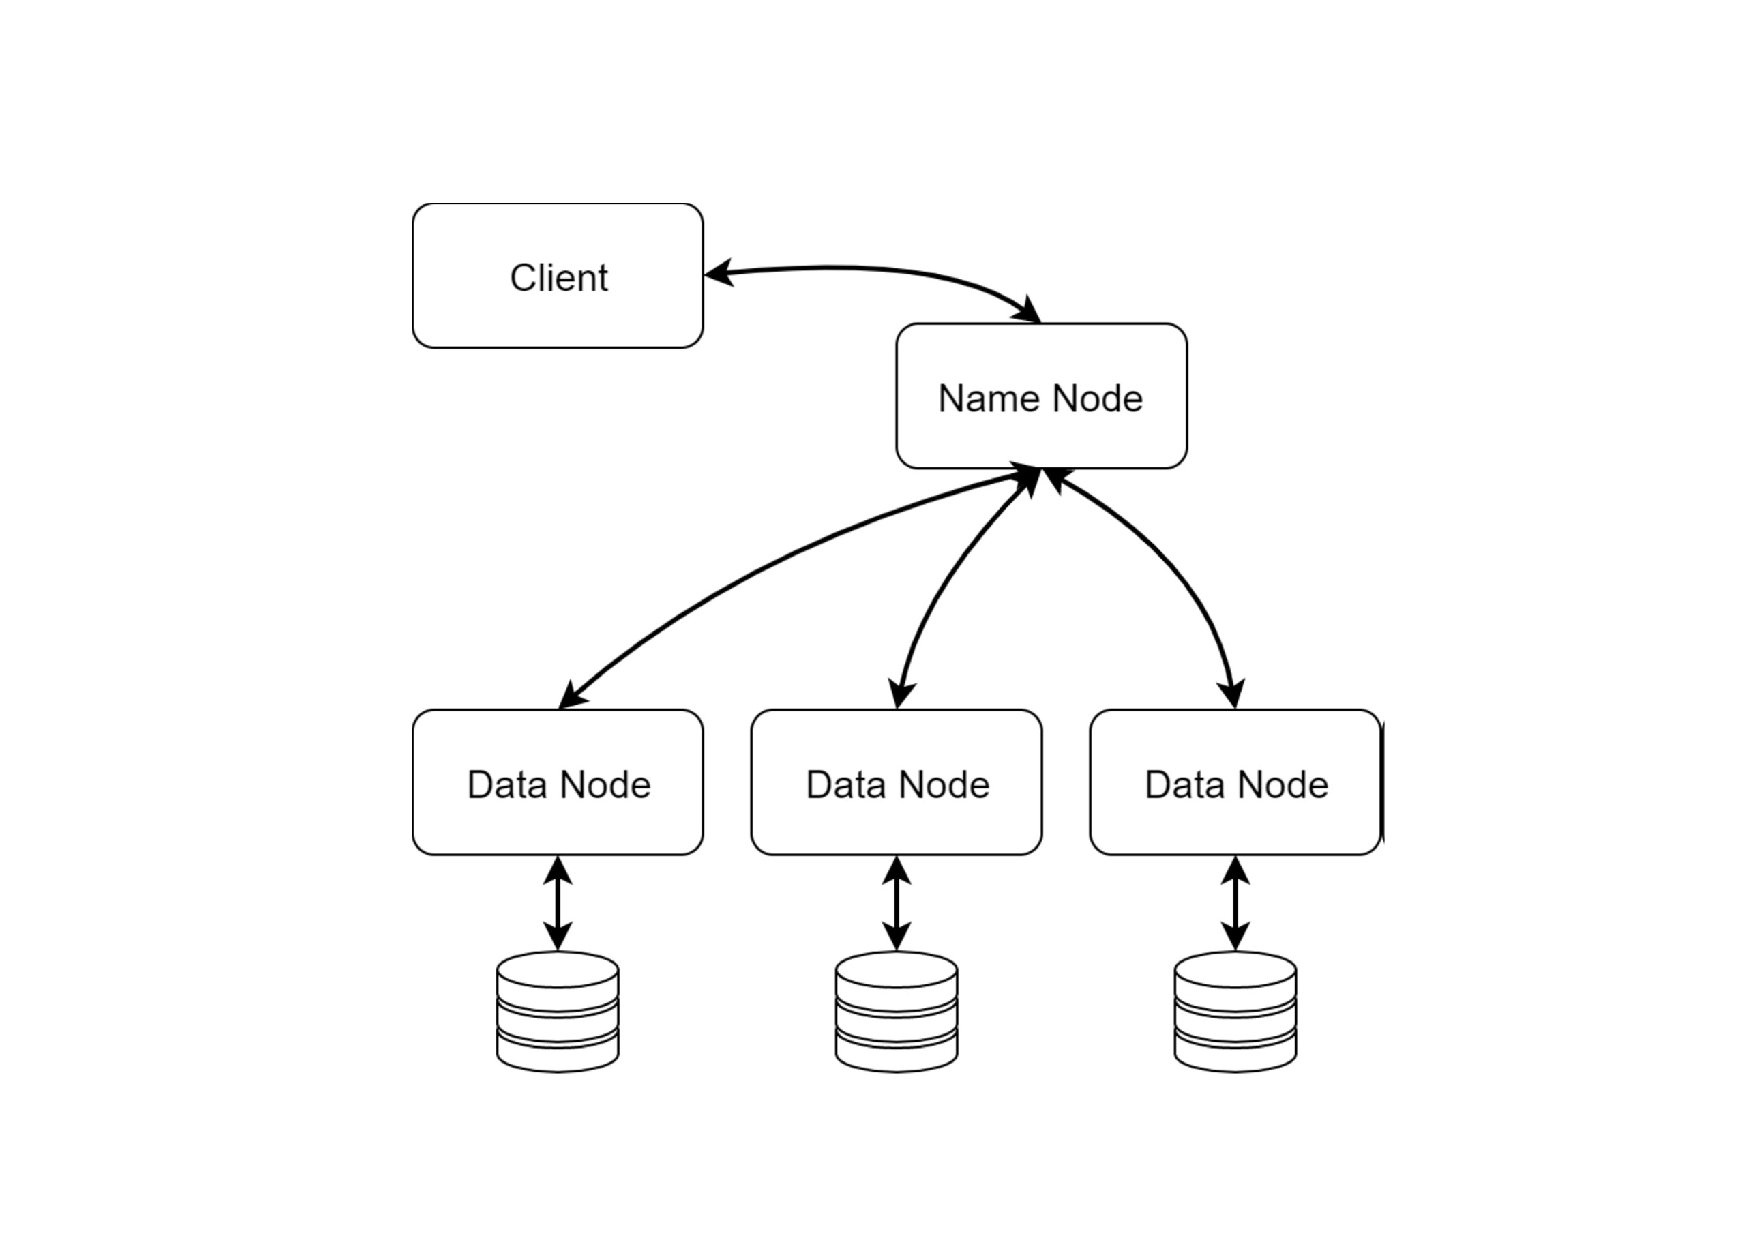
\includegraphics[width=\columnwidth]{Images/hdfs_1.pdf}  
	\vspace{-1cm}
	\caption[HDFS Node Strucure]{HDFS Node Strucure.}
	\label{fig:hdfsNodeStruct}
\end{figure}
HDFS exposes a filesystem namespace and allows user data to be stored in files and retrieved. Clusters are composed by one master and multiple slaves, as shown in \myFig{fig:hdfsNodeStruct}.

The master provides a single Name Node (NN), that manages
the file system namespace and regulates access to the files by clients.
NN executes filesystem operations such as file open, close, rename, 
and keeps track of the mapping between blocks and Data Node (DN). 
File stored in HDFS are split into blocks, that are stored in the Data Node (DN). Data Node (DN) represent the slaves, and manage the storage attached to the node they are running on. They serve read and write operation requests from the clients, but also can perform block creation, deletion and replication. Block replication is a way to improve fault tolerance.

\subsection{Batch Processing: Spark}\label{sec:spark}
Apache Spark is an open source framework for distributed computation 
~\cite{misc:ApacheSpark} provides an Application Programming Interface (API) that provides implicit data parallelism and fault tolerance. With respect to the MapReduce paradigm, the in-memory multilevel primitives of Spark allow to have up to 100 times better performance. Spark can run as standalone or on a cluster manager such as Apache Hadoop Yarn or Apache Mesos. It also needs a distributed storage and can natively use HDFS and other solutions. 

Spark was designed as a unified engine for distributed data processing. Its programming model extends the MapReduce with a data sharing abstraction called Resilient Distributed Dataset (RDD). This abstraction allows the processing many different workloads, including SQL, streaming, machine learning and graph processing. 

The generality of the Spark approach allows an easy development of applications through the use of its API, and an easy combination of  processing tasks. Previous distributed frameworks required data to be written to disk before using them in other processes. Spark allows the reuse of the data, often kept in memory.

RDDs are fault-tolerant collections of objects partitioned across the cluster that can be processed in parallel. Users create RDDs by applying "transformation" operations like map, filter and group-by on the input data. RDDs can be backed by a file obtained from an external storage. RDD are evaluated in a lazy mode. This allows the construction of an efficient plan to execute the computation requested by the user. 

Every transformation operation returns a new RDD, that represents the result of the computation, however the computation is not executed immediately after the transformation request is encountered, but only when a Spark action is met. When an "action" is requested by the user code, Spark checks the entire graph of the transformation and uses it to create an efficient execution plan. For example, if there are many filters and maps in a row, Spark can merge them together and execute as a single operation.

RDDs also offer an explicit support by default non-persistent data sharing among the computations. This capability is one of the main differences between Spark and the previous  models like MapReduce. Data sharing capability allows huge speedups, up to 100 times, in particular when executing interactive queries and iterative algorithms.
RDDs can also recover automatically from a failure. Traditionally, fault tolerance in distributed computing was achieved by means of data replication and checkpointing. Spark instead uses a different approach called lineage. Each RDD keeps track of its transformation graph used to generate the RDD and re-executes the transformation operations on the base data to recover every lost partition. Data recovery based on lineage is significantly more efficient than replication in case of data-intensive workload. In general, recovering lost partitions is faster than re-executing the entire program. 

Spark was designed to support different external systems for persistent storage, usually it is used in conjunction with a clustered file system like HDFS. Spark is designed as a storage-system-agnostic engine, to make it easy to run computations against data from different sources.
\begin{figure}
	\vspace{-1cm}
	\centering
	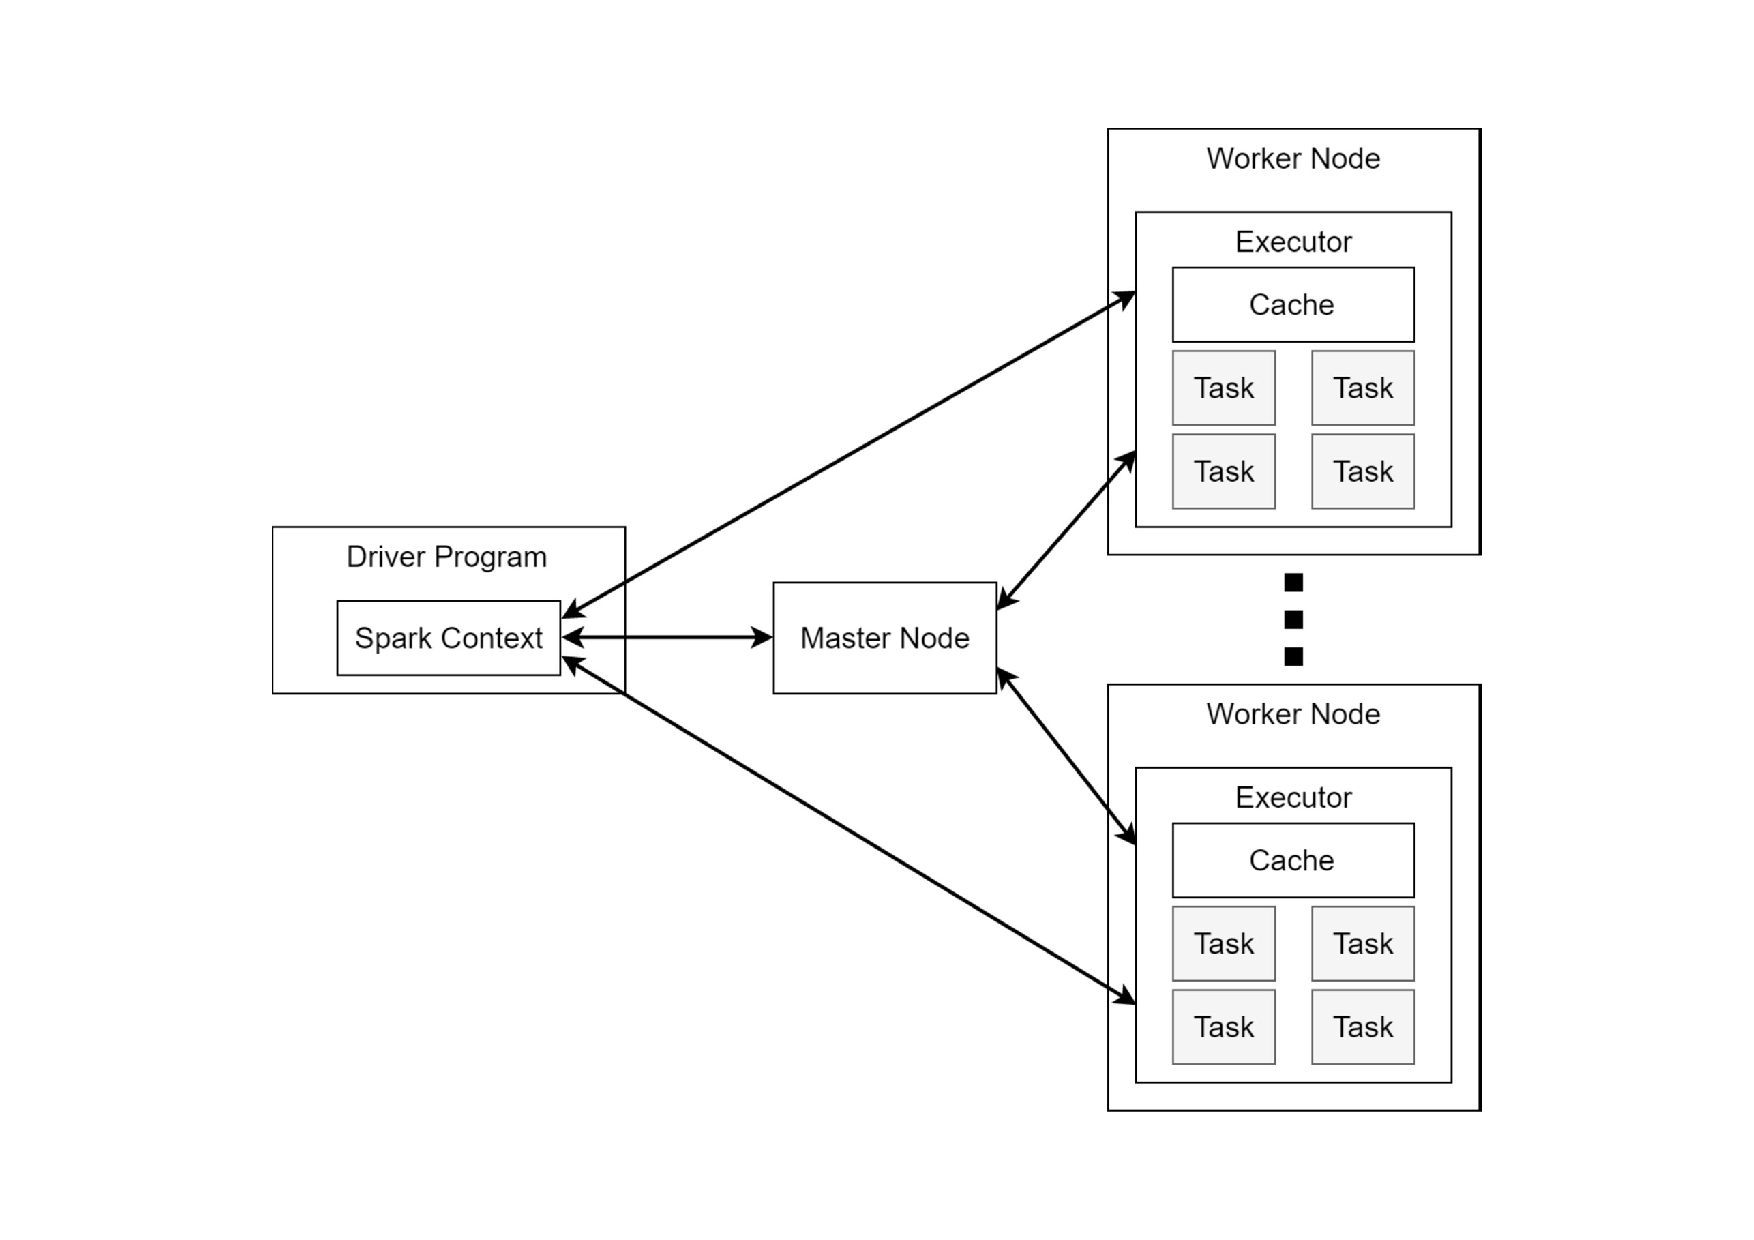
\includegraphics[width=\columnwidth]{Images/spark_standalone_architecture.pdf}  
	\vspace{-1.5cm}
	\caption[Spark Standalone Architecture]{Spark Standalone Architecture.}
	\label{fig:sparkStandaloneArchitecture}
\end{figure}

Different high-level libraries have been developed in order to simplify
the creation of programs that can run in Spark framework.
\begin{itemize}
	\item SQL and DataFrames: support for relational queries, that are the most common data processing paradigm
	\item Spark Streaming: implements incremental stream processing using a model called "discretized streams", input data is split into micro batches
	\item GraphX: graph computation interface
	\item MLlib: machine learning library, more than 50 common algorithms for distributed model training
\end{itemize}

Spark architecture implements the master/worker paradigm  (\myFig{fig:sparkStandaloneArchitecture}). A master server accepts data and processing request, splits them into smaller chunks of data and simpler actions that can be executed in parallel by the workers. 

A Spark application is executed by a driver program, that makes the user code executable on the computing cluster using a SparkContext. The driver program is responsible for managing the job flow and scheduling tasks that will run on the executors. The SparkContext will split the requested operations in tasks the can be scheduled for distributed execution on the workers. 

When a SparkContext is created, a new Executor process is created on each worker. An executor is a separate Java Virtual Machine (JVM) that runs for the entire lifetime of the Spark application, executes tasks using a thread pool and store data for its Spark application. Communication between the SparkContext and the other components is performed using a shared bus.
\begin{figure}
	\vspace{-1.5cm}
	\centering
	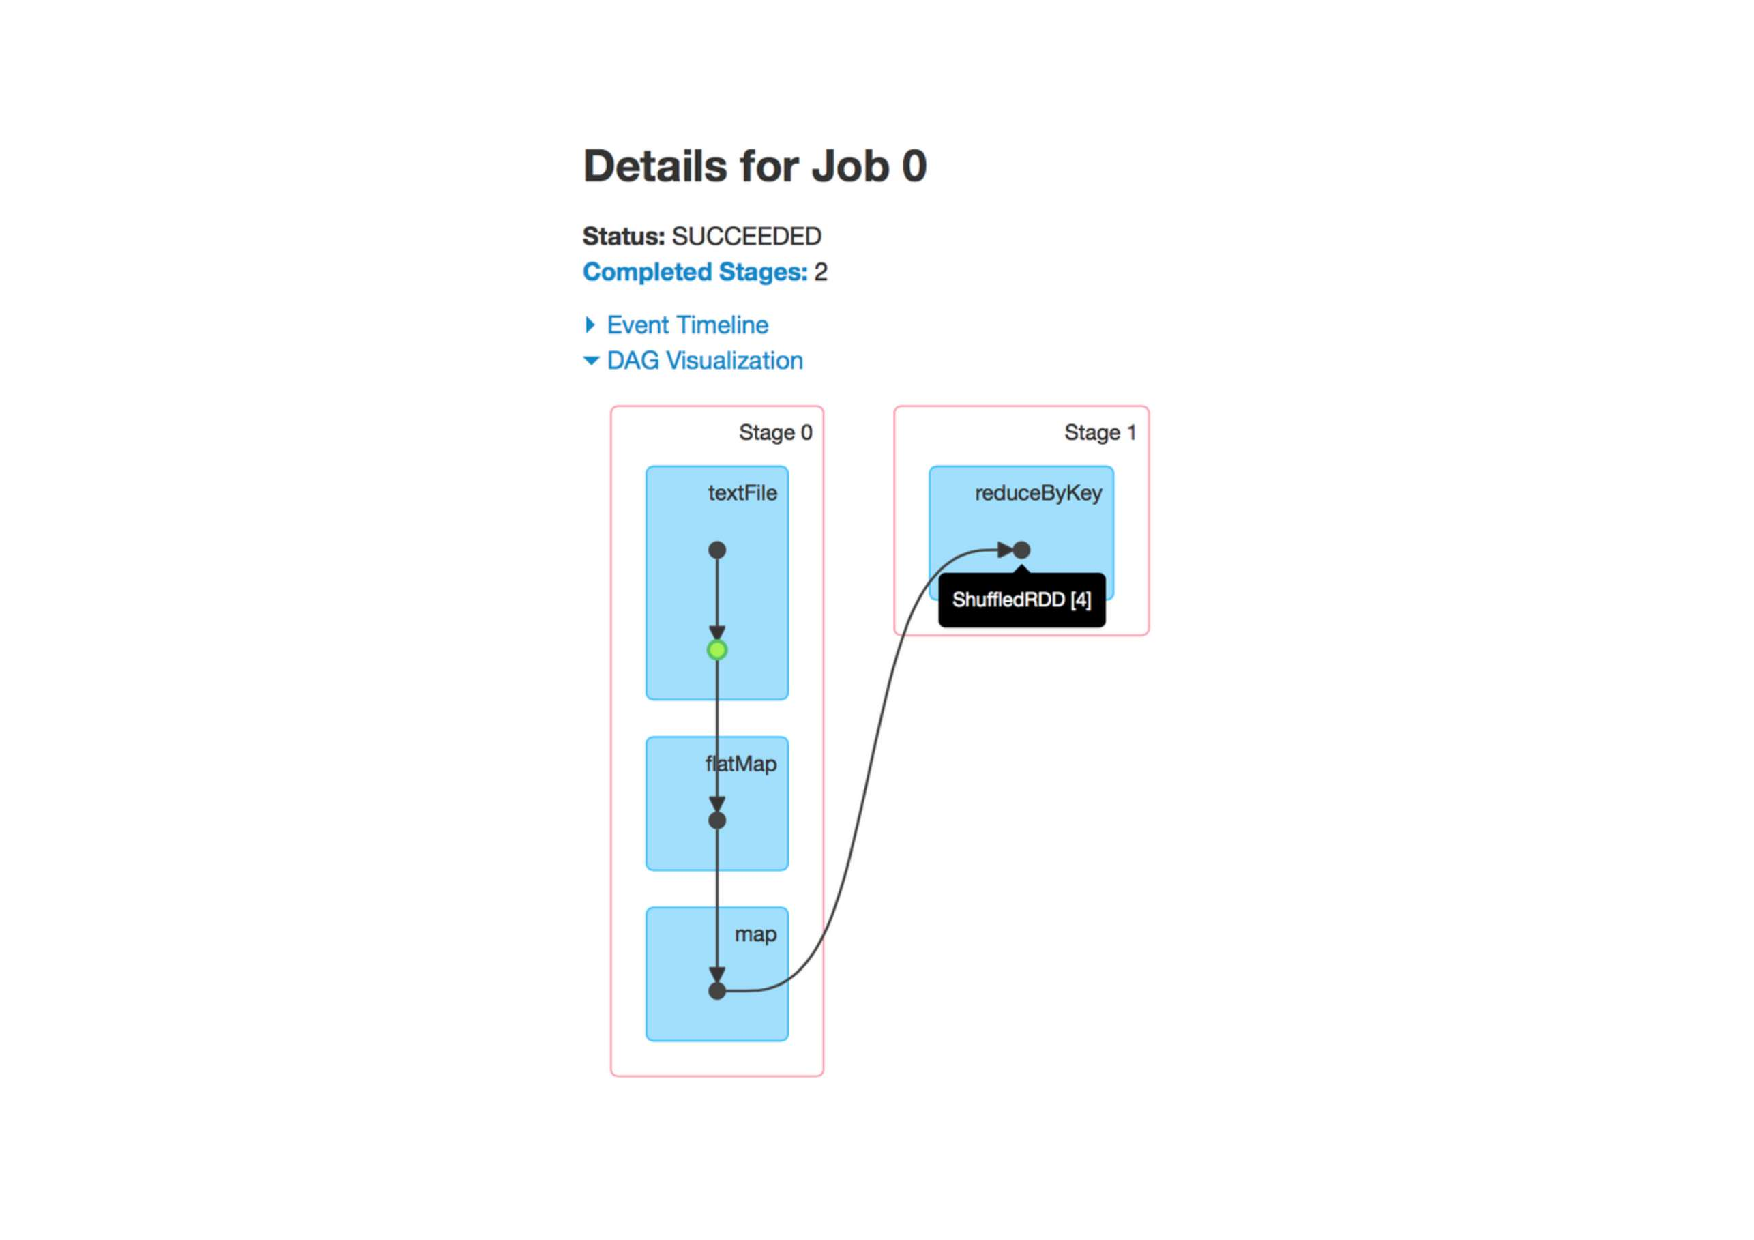
\includegraphics[width=\columnwidth]{Images/spark_dag_example.pdf}  
	\vspace{-1.5cm}
	\caption[Spark DAG Example]{Spark DAG Example.}
	\label{fig:sparkDAGExample}
\end{figure}

When an application is submitted to Spark, it is divided in multiple jobs. Jobs are delimited by Spark actions in the application code. Spark actions are those operations that return a value to the driver program after running a computation on the data set.

For each job, a Directed Acyclic Graph (DAG) is created to keep track of the RDDs that are materialized inside the job. DAG nodes represent the RDDs, while arcs represent transformations, that are the operations that create new datasets from existing ones.

The application steps inside a single job are further organized into stages, that are delimited by operations requiring data reshuffling, that will break locality. Spark distinguishes between narrow transformations, that do not reshuffle data (e.g., map, filter), and wide transformations, that require data reshuffling (e.g., reduceByKey). 

Stages are also used to produce intermediate result that can be persisted to memory or mass storage to avoid re-computation. When all stages inside a job have been identified, Spark can determine which parallel tasks need to be executed for each stage, and schedule them for operation on the executors. Spark creates one task for each partition of the RDD received in input by a stage.

\lstinputlisting[
firstline=1,
lastline=4,
float=tb,
language=Java,
tabsize=2,
numbers=left,
numberstyle=\tiny,
stepnumber=1,
numbersep=5pt,
caption={Spark word count application example.}, 
captionpos=t,
label=lst:wordCount
]{CodeFiles/wordCount.java}

\MyFig{fig:sparkDAGExample} shows a simple DAG representing the single job of the word count application presented in \MyListing{lst:wordCount} \cite{misc:SparkApplication}. The image is taken from SparkWeb UI. Through a textFile operation, the input file is read from HDFS. Then a flatMap operation is applied to split each of the lines of the document into words. Then, a map is used to create (’word’, 1) pairs. Finally, a reduceByKey operation is performed to count the occurrences of each word. The blue boxes represent the Spark operations that the user calls in his code, while the dots represent the RDDs that are created as a result of these operations. Operations are grouped into stages, represented by the boxes with a red border. The job has been divided into two stages because the reduceByKey transformation requires the data to be shuffled. The green dot represents a cached RDD, in particular the data read from HDFS has been cached, in this way future computations on this RDD can be done faster since data will be read from memory instead of HDFS. The default deployment of Spark is in standalone mode, that is using its embedded cluster manager. 

%\subsection{Streams Processing: Flink}\label{sec:flink}
\subsection{Stream Processing}\label{sec:stream_processing}
\begin{figure}[t]
	\vspace{-1.5cm}
	\centering
	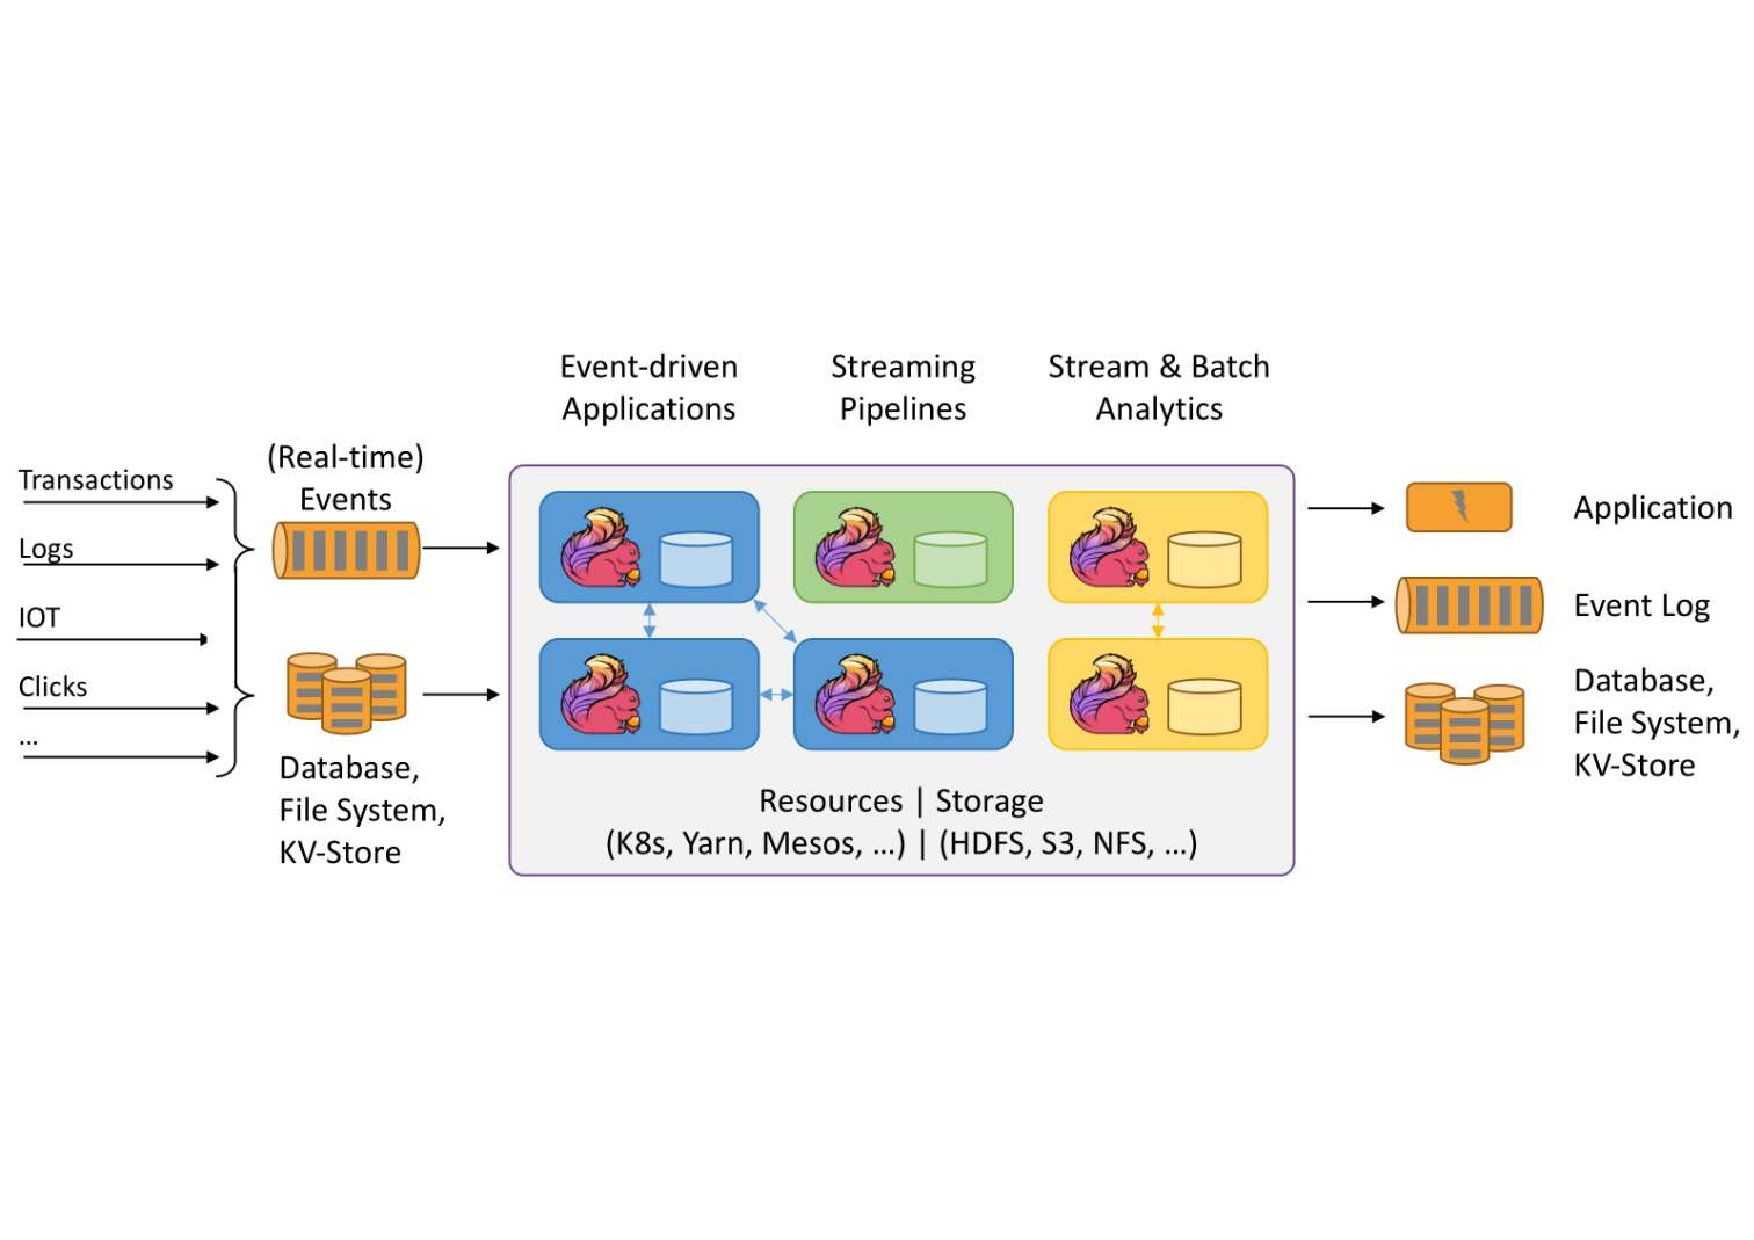
\includegraphics[width=\columnwidth]{Images/apache_flink.pdf}
	\vspace{-2.5cm}
	\caption[Apache Flink® - Stateful Computations over Data Streams.]{Apache Flink® - Stateful Computations over Data Streams.}
	\vspace{1.5cm}
	\label{fig:apache_flink}
\end{figure}
\begin{figure}
	\vspace{-2.5cm}
	\centering
	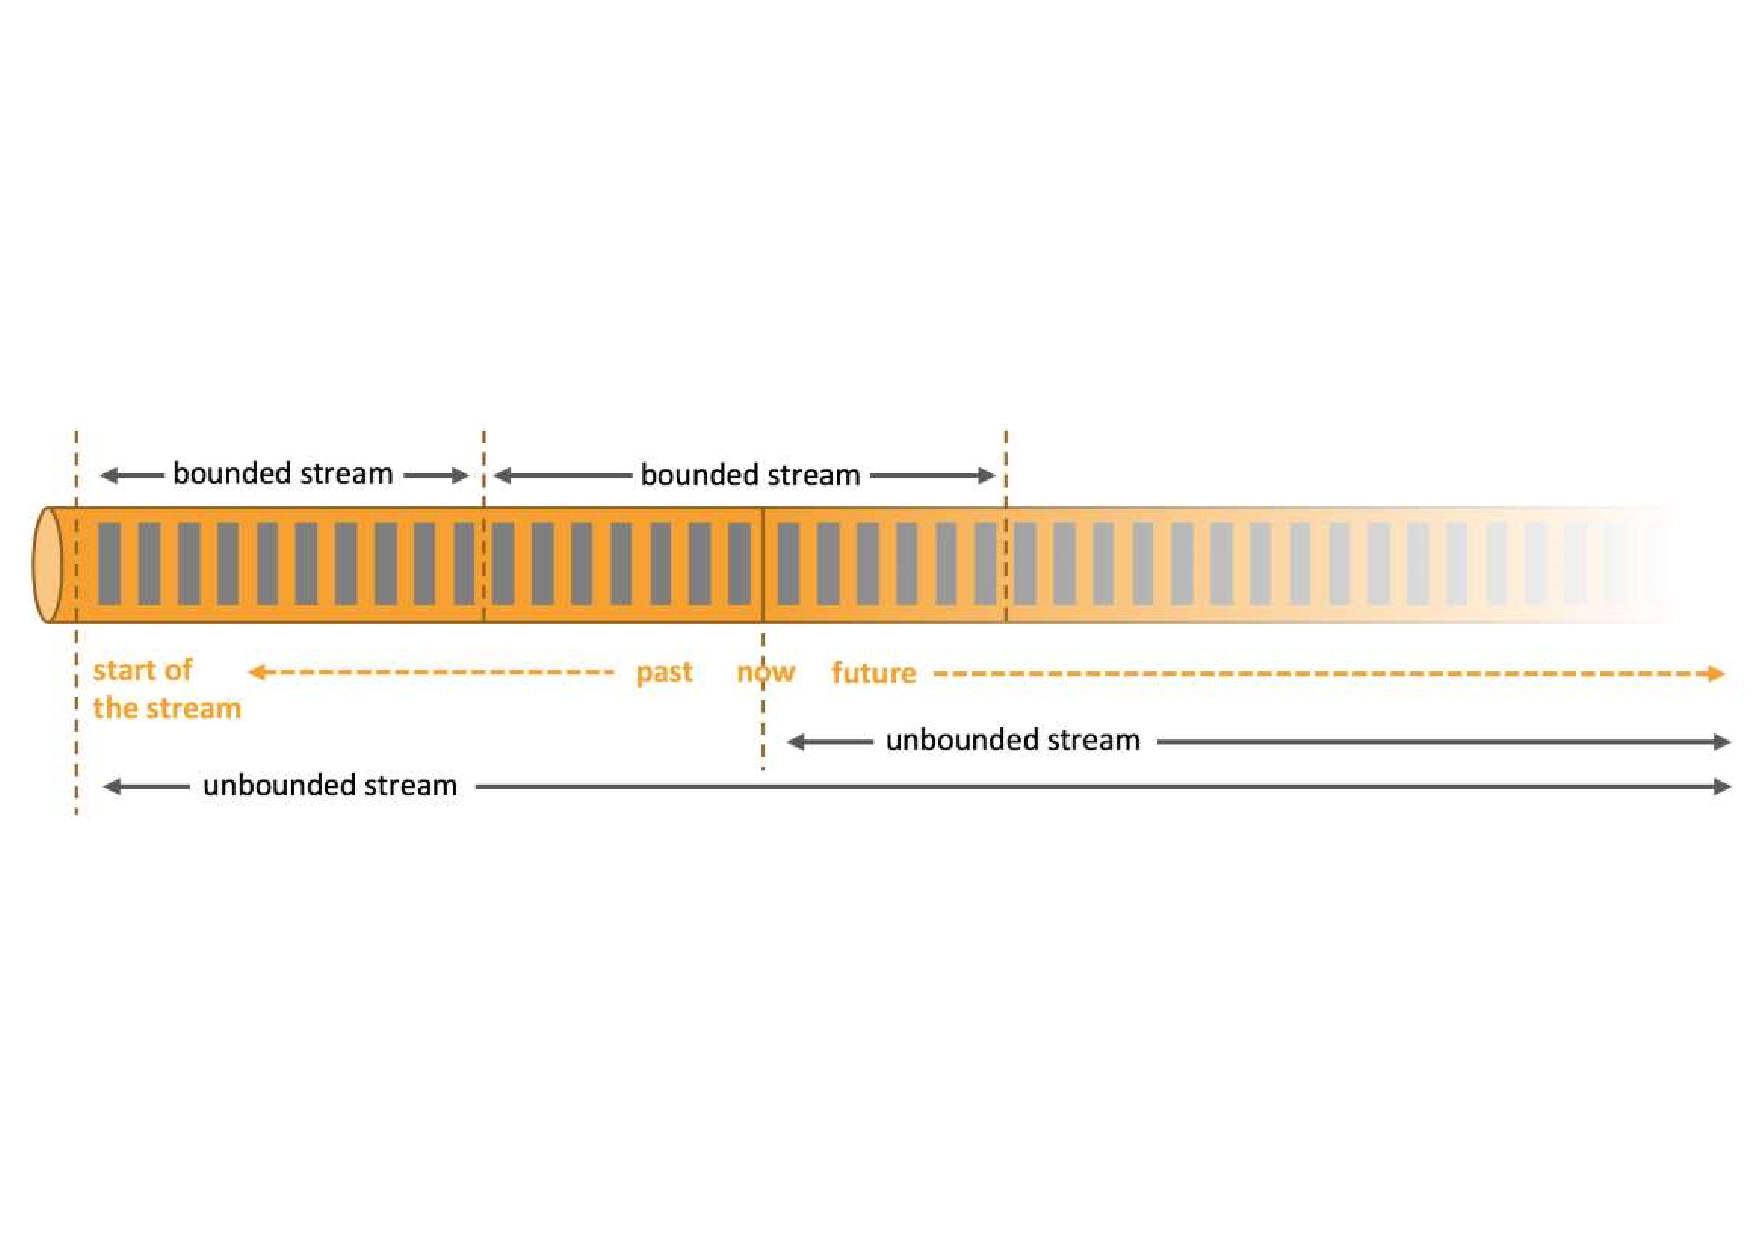
\includegraphics[width=\columnwidth]{Images/apache_flink_data_streams.pdf}
	\vspace{-3cm}
	\caption[Apache Flink® - Bounded \& Unbounded Data Streams.]{Apache Flink® - Bounded \& Unbounded Data Streams.}
	\label{fig:apache_flink_data_streams}
\end{figure}

Apache Flink~\cite{misc:ApacheFlink} is a framework and distributed processing engine for stateful computations over unbounded and bounded data streams. It can run in any commonly used cluster environments, computes at in-memory speed and manages data at any scale.

Flink’s architecture can process unbounded and bounded data. Sensors data, server logs or user interactions on a website or mobile application, credit card transactions, all of these data are generated as streams of data.

Data can be processed as unbounded or bounded streams~\cite{misc:ApacheFlinkArchitecture}. 

Unbounded streams have a start but no defined end. They do not terminate and provide data as it is generated. Unbounded streams must be continuously processed, i.e., events must be managed right after they have been read. %It is not possible to wait for all input data to arrive because the input is unbounded and will not be complete at any point in time. Processing unbounded data often requires that events are processed in a specific order, such as the order in which events occurred, to be able to reason about result completeness.

Bounded streams have a defined start and end. Bounded streams can be processed by reading all data before performing any computations. Ordered reading is not required to process bounded streams because a bounded data set can always be sorted. Processing of bounded streams is also known as batch processing.


%Apache Flink excels at processing unbounded and bounded data sets. Precise control of time and state enable Flink’s runtime to run any kind of application on unbounded streams. Bounded streams are internally processed by algorithms and data structures that are specifically designed for fixed sized data sets, yielding excellent performance.

%\subsection{Streams Processing: Storm}\label{sec:storm}

\begin{figure}[t]
	\vspace{-1.5cm}
	\centering
	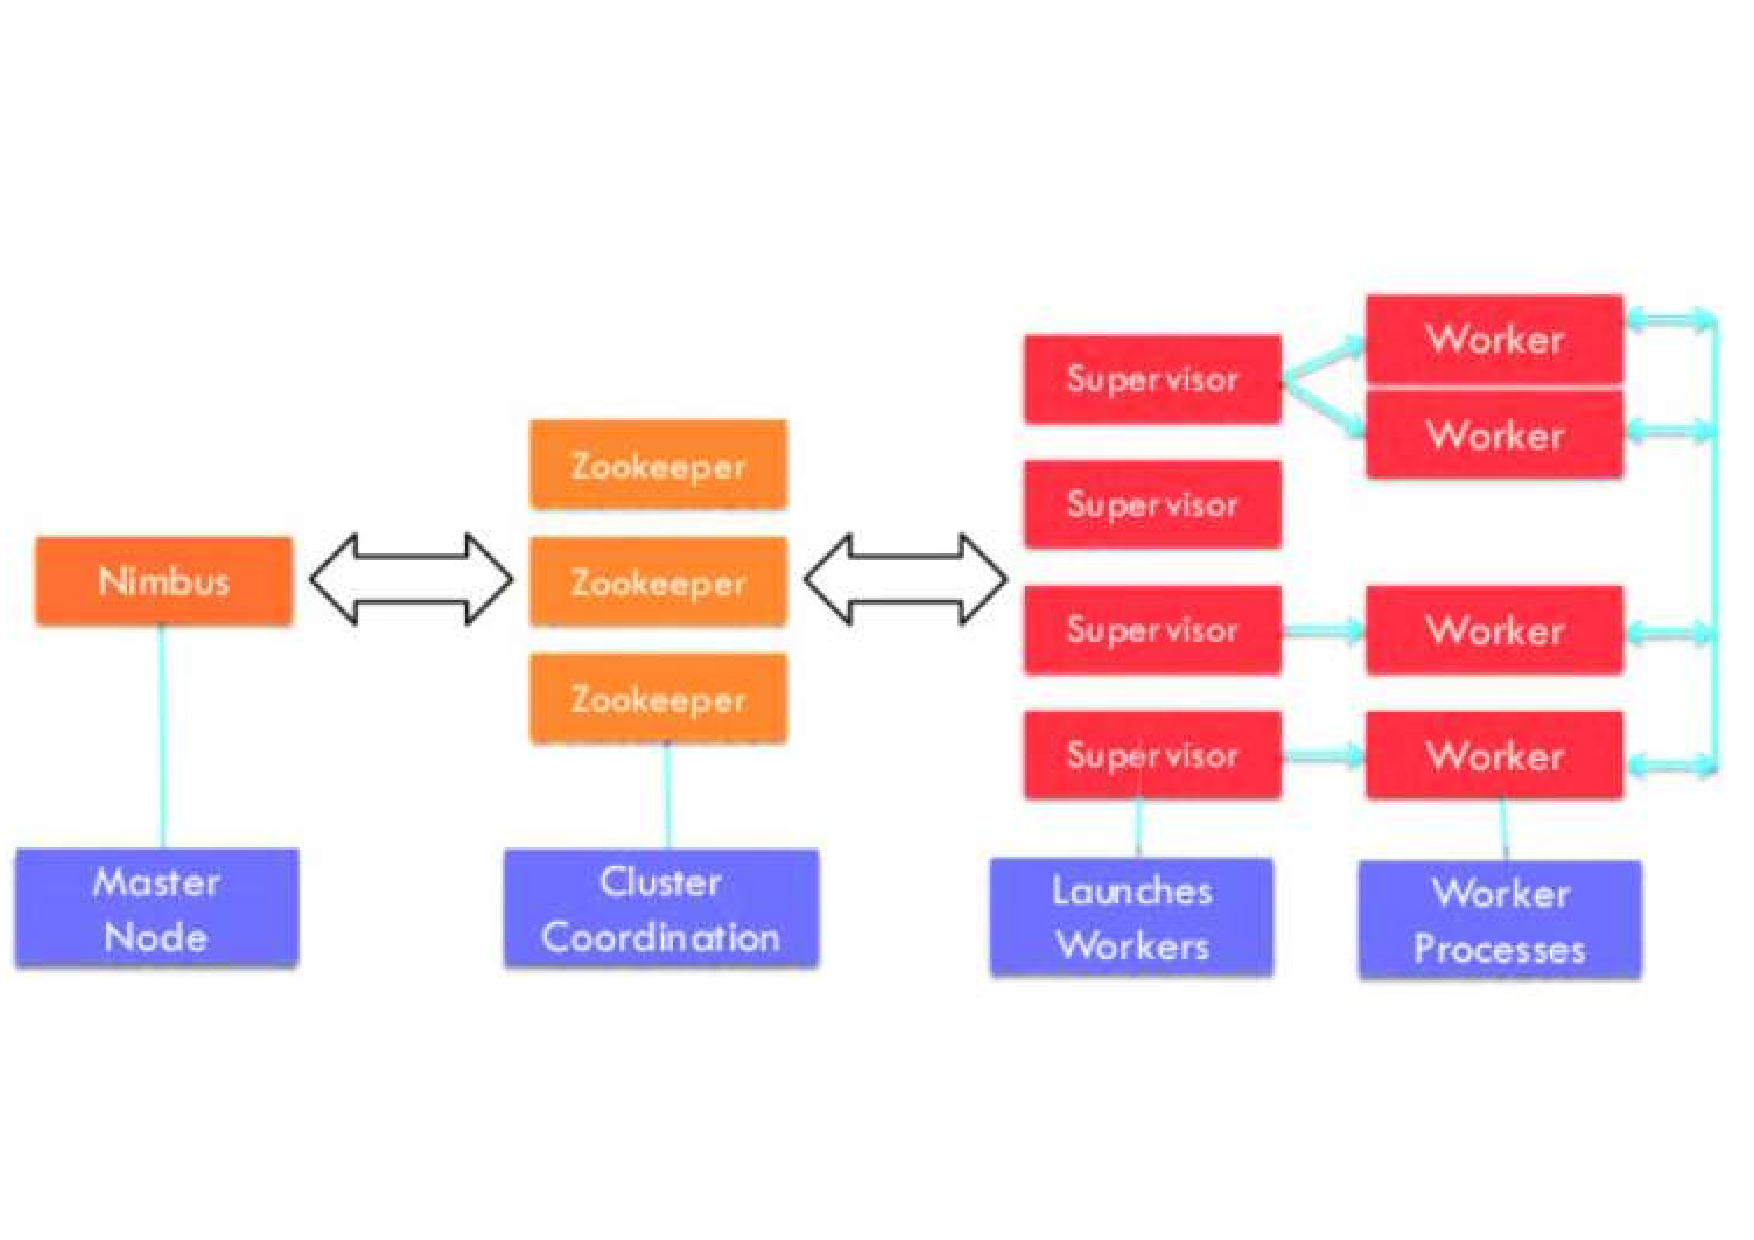
\includegraphics[width=\columnwidth]{Images/apache_storm.pdf}
	\vspace{-2cm}
	\caption[Apache Storm.]{Apache Storm.}
	\label{fig:apache_storm}
\end{figure}
\begin{figure}
	\vspace{-0.5cm}
	\centering
	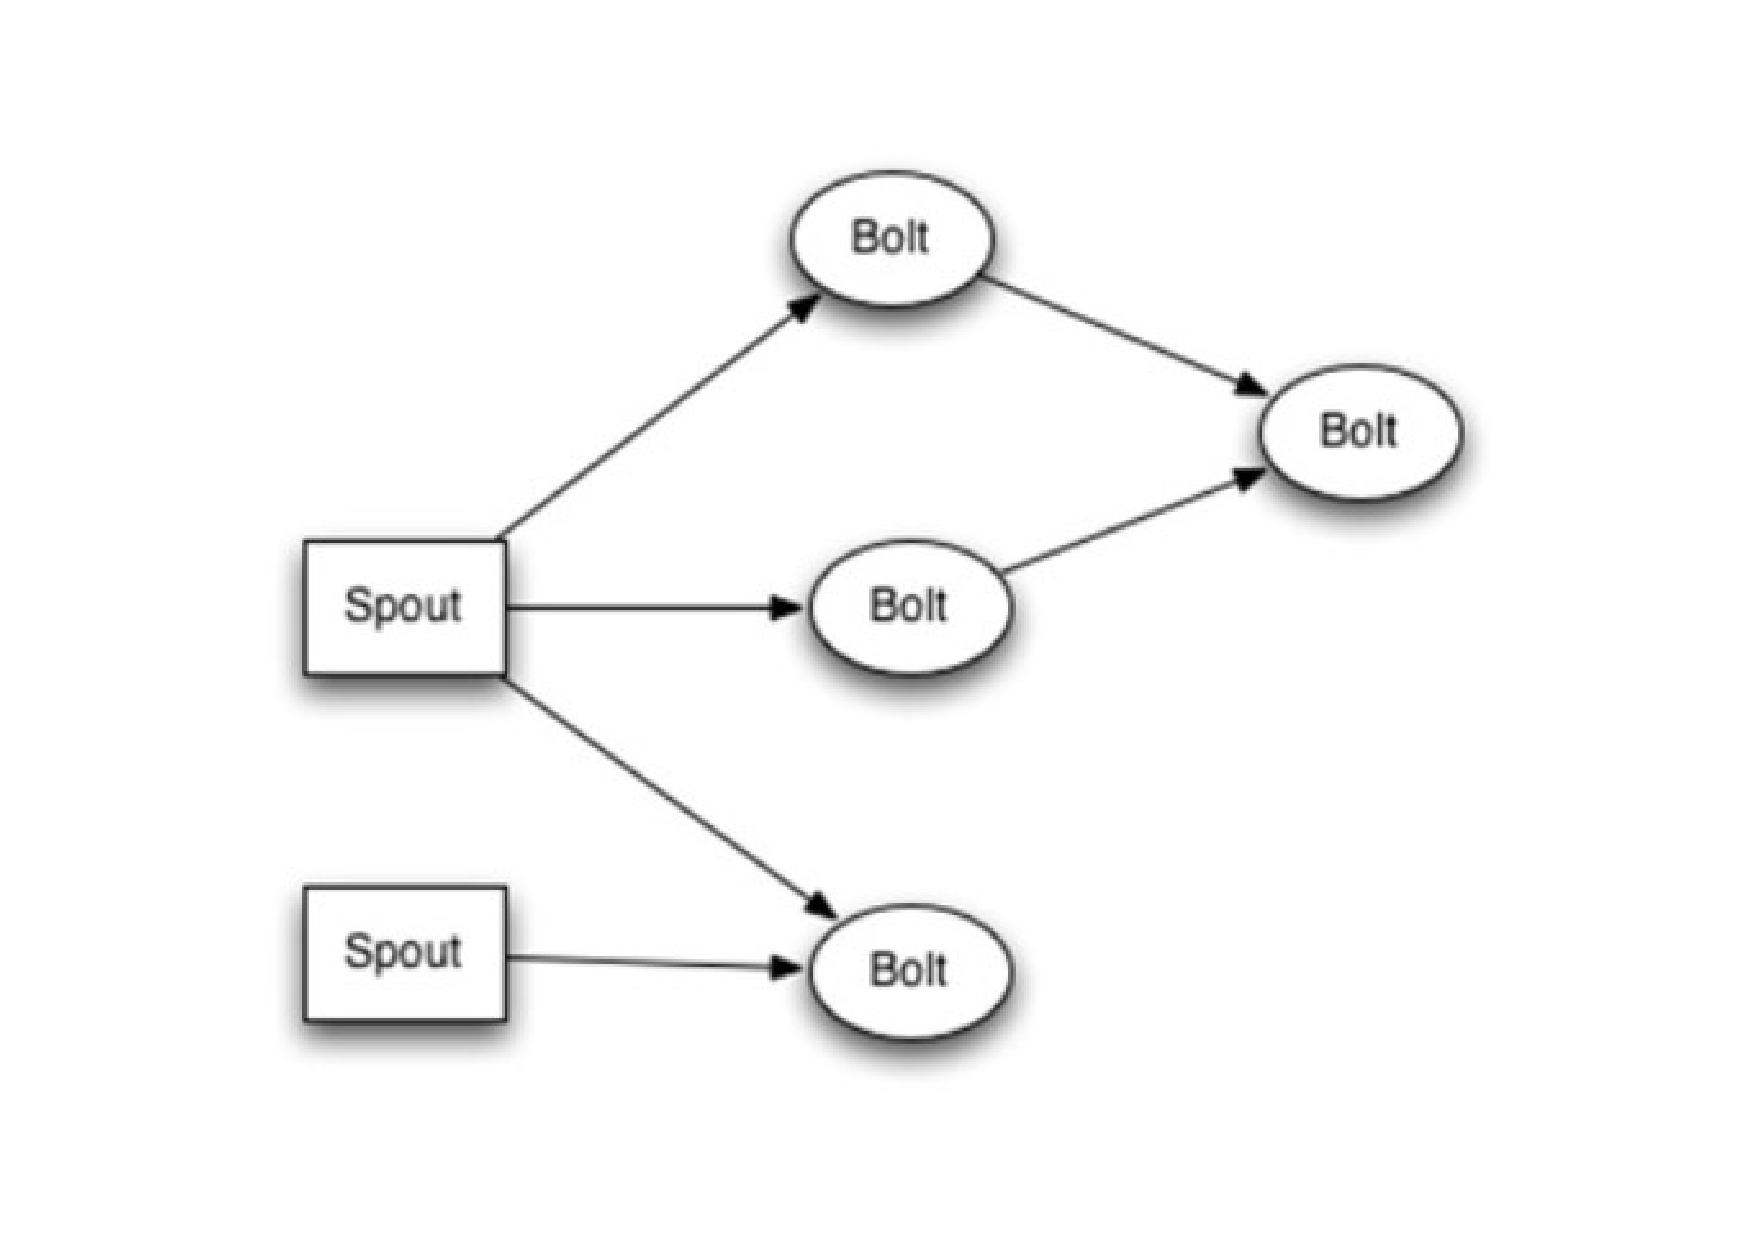
\includegraphics[width=\columnwidth]{Images/apache_storm_components_abstraction.pdf}
	\vspace{-1.5cm}
	\caption[Apache Storm Components Abstraction.]{Apache Storm Components Abstraction.}
	\label{fig:apache_storm_components_abstraction}
\end{figure}

Apache Storm~\cite{misc:ApacheStorm} is a free and open source distributed realtime computation system. Storm makes it easy to reliably process unbounded streams of data, doing for realtime processing what Hadoop did for batch processing. Storm is simple, can be used with any programming language, and is easy to use.

%Storm has many use cases: realtime analytics, online machine learning, continuous computation, distributed RPC, ETL, and more. Storm is fast: a benchmark clocked it at over a million tuples processed per second per node. It is scalable, fault-tolerant, guarantees your data will be processed, and is easy to set up and operate.

%Storm integrates with the queueing and database technologies commonly used. A Storm topology consumes streams of data and processes those streams in arbitrarily complex ways, repartitioning the streams between each stage of the computation however needed. 

The Apache Storm architecture is quite similar to that of Hadoop. However there are certain differences which can be better understood by getting a closer look at its cluster in \MyFig{fig:apache_storm}. 
%\textbf{Nodes} - 
There are two types of nodes in Storm cluster similar to Hadoop:
\begin{itemize}
	\item {Master node - }The master node of Storm runs a daemon called ‘Nimbus’, which is similar to the ‘Job Tracker’ of Hadoop cluster. Nimbus is responsible for distributing codes, assigning tasks to machines and monitoring their performance.
	\item {Worker node – }Similar to the master node, the worker node also runs a daemon called ‘Supervisor’ which is able to run one or more worker processes on its node. %Each supervisor works assigned by Nimbus and starts and stops the worker processes when required. Every worker process runs a specific set of topology which consists of worker processes working around machines. Since Apache Storm does not have the abilities to manage its cluster state, it depends on \textbf{Apache Zookeeper} for this purpose. Zookeeper facilitates communication between Nimbus and Supervisors with the help of message acknowledgements, processing status, etc.
\end{itemize}
%\textbf{Storm Components/Abstractions} (see  \MyFig{fig:apache_storm_components_abstraction})
There are basically four components which are responsible for performing the tasks(see  \MyFig{fig:apache_storm_components_abstraction}):

\begin{itemize}
	\item Topology – Storm Topology can be described as a network made of \textbf{spouts} and \textbf{bolts}. It can be compared to the Map and Reduce jobs of Hadoop. Spouts are the data stream source tasks and Bolts are the accrual processing tasks.% Every node in the network consists of processing logic’s and links to demonstrate the ways in which data will pass and the processes will be executed. Each time a topology is submitted to the storm cluster, Nimbus consults the supervisor nodes about the worker nodes. 
	\item Stream – One of the basic abstractions of the storm architecture is stream which is an unbounded pipeline of tuples.% A tuple can be defined as the fundamental component in the Storm cluster containing a named list of the values or elements.  
	\item Spout – It is the entry point or the source of streams in the topology. %It is responsible for getting in touch with the actual data source, receiving data continuously, transforming those data into actual stream of tuples and finally sending them to the bolts to be processed.
	\item Bolt - Bolts keep the logic required for processing. %These are responsible for emitting the streams for processing by other bolts and saving or sending the data for storage. These are capable of running functions, filtering tuples, aggregating and joining streams, linking with database, etc.
\end{itemize}

\section{Runtime Management of Big Data Applications}\label{sec:runtime_mgmt_big_data_apps}
Big data applications requires system scalability, fault tolerance and  availability~\cite{articleBigData:2017}. 

\textit{Scalability} means the ability to maintain an approximate linear relationship between the size of processed data and the amount of consumed resources. 

\textit{Fault tolerance} is a challenge, especially when systems are complex and involve many networked nodes. By means of hardware virtualization, cloud computing services satisfies all the requested requisites, and the \textit{elasticity} and redundancy it provides  also enable big data application high availability, scalability and fault tolerance.

Another very important feature of big data applications is the \textit{Quality of Service} or \qos.

\qos definition for IT applications differ by application type. Interactive applications are usually assessed according to response time or throughput, and their fulfillment depends on the intensity and variety of the incoming requests. 

Big data applications might require a single batch computation on a very large dataset, thus \qos must consider the execution of a single run. In this domain \qos is often called \textit{deadline}, or the maximum allowed duration of the computation. 

We have mentioned %availability, fault tolerance and availability as fundamental requirements and 
\qos as a measure of the capability to meet a user-defined deadline when processing big data. Many factors influence the duration of an application execution, surely resource allocation greatly influences the duration. 

The challenges introduced by big data require resilient, flexible and self-adapting software systems~\cite{DeLemos2013}. Hence, \textit{autonomic system}s and \textit{self-adaptation} has increasingly captured the attention of researchers ~\cite{Weyns:2012:CSE:2666795.2666811}. These systems automatically react to changes in the environment, or in their own state, and change their behaviour to satisfy functional and non-functional requirements. Meeting requirements in complex and variable execution environments is a difficult task that can be tackled at design time or at runtime. At runtime the adaptation is very often obtained by using a well-known process called MAPE~\cite{MAPE}, a control loop composed of four phases: monitoring, analysis, planning and execution.

One of the challenges that modern software systems face is the provisioning and optimization of resources to meet a varying demand, generated by are increasingly common phenomena like fluctuating workloads, unpredictable peaks of traffic and unexpected changes. Service providers cannot disregards these factors if they want to cope with the challenge of satisfying functional and non-functional requirements, usually defined in SLAs (Service Level Agreements). Hence the need arises for an automatic adjustment of system resources allocation to avoid resource saturation and unresponsiveness, users dissatisfaction and unnecessary costs. This paradigm is called elastic resource provisioning~\cite{Dustdar2011, Zhang2010, Sehgal2012, Herbst2013}.

Many approaches about elastic systems and dynamic resource allocation were proposed both in the industry and in academia. In modern technology elasticity is often enabled by cloud computing that gives to an application a theoretical infinite degree of scalability. However considering only resources is rather restrictive because of the many factors that impact application during their runtime life-cycle. In fact Dustdar et al.~\cite{Dustdar2011} argue that elastic computing should be designed by considering three dimensions: quality, resources and cost.  Quality elasticity considers how quality is affected by a change in resource availability. Instead cost elasticity measures how resource provision is affected when a change in cost happens. 

Cloud computing services provide the needed level of fault tolerance and availability required by big data applications. In the remainder of this chapter we present an overview of popular big data frameworks that can leverage cloud computing solutions and how they address elastic resource allocation to satisfy functional and non-functional application requirements. The resulting scenario represent the base for our work, where we will consider quality elasticity and not cost elasticity aspects. 

This thesis shows how the application of lightweight symbolic execution tecniques to deadline-based \qos constrained multi-DAG big data applications helps reduce the number of deadline violations and allocate resources more efficiently.


\section{Elastic Resource Provisioning}
\label{Section:Introduction:ElasticProvisioning}

The word \textit{elasticity} comes from physics and is defined as the ability of an object or material to resume its normal shape after being stretched or compressed. In computing, elasticity has a similar meaning and is used to characterize \textit{autonomic systems}. Herbst et al.~\cite{Herbst2013} defines elastic provisioning as reported below.
\begin{quote}
	\textit{\textbf{Elasticity} is the capability of a system to adapt to workload changes by provisioning or de-provisioning resources automatically such that at each point in time the available resources match the current demand as closely as possible}.
\end{quote}

A system is in an \textit{under provisioned} state if it allocates less resources than required by the current demand; it is in an \textit{over provisioned} state if allocates more resources than required. Moreover, elasticity is determined by four attributes:

\begin{itemize}
	\item \textit{Autonomic Scaling}: the adaptation process used to control the system.
	\item \textit{Elasticity Dimensions}: the set of scaled resources in the adaptation process.
	\item \textit{Resource Scaling Units}: the minimum amount of allocable resources to each dimension.
	\item \textit{Scalability Bounds}: the lower and the upper bound on the amount of resources that can be allocated to each dimension.
\end{itemize}

Additionally, two aspects must be considered in evaluating the elasticity degree of a system: speed and precision. 

\textbf{Speed of scaling up/down:} the time it takes to switch from an underprovisioned/overprovisioned state to an optimal or overprovisioned/underprovisioned state respectively. 

\textbf{Precision of scaling}: the absolute deviation of the current amount of allocated resources from the actual resource demand.

Scalability and efficiency are terms related to elasticity, nevertheless they differ by the following aspects:
 
\textbf{Scalability}, although is a prerequisite for elasticity, it does not consider the temporal aspects (how fast and how often) and the granularity of the adaptation actions.

\textbf{Efficiency}, contrary to elasticity, takes in account all the types of resources employed to accomplish a certain amount of work, not only the resources scaled by the adaptation actions. 

\begin{figure}
	\vspace{-1.5cm}
	\centering
	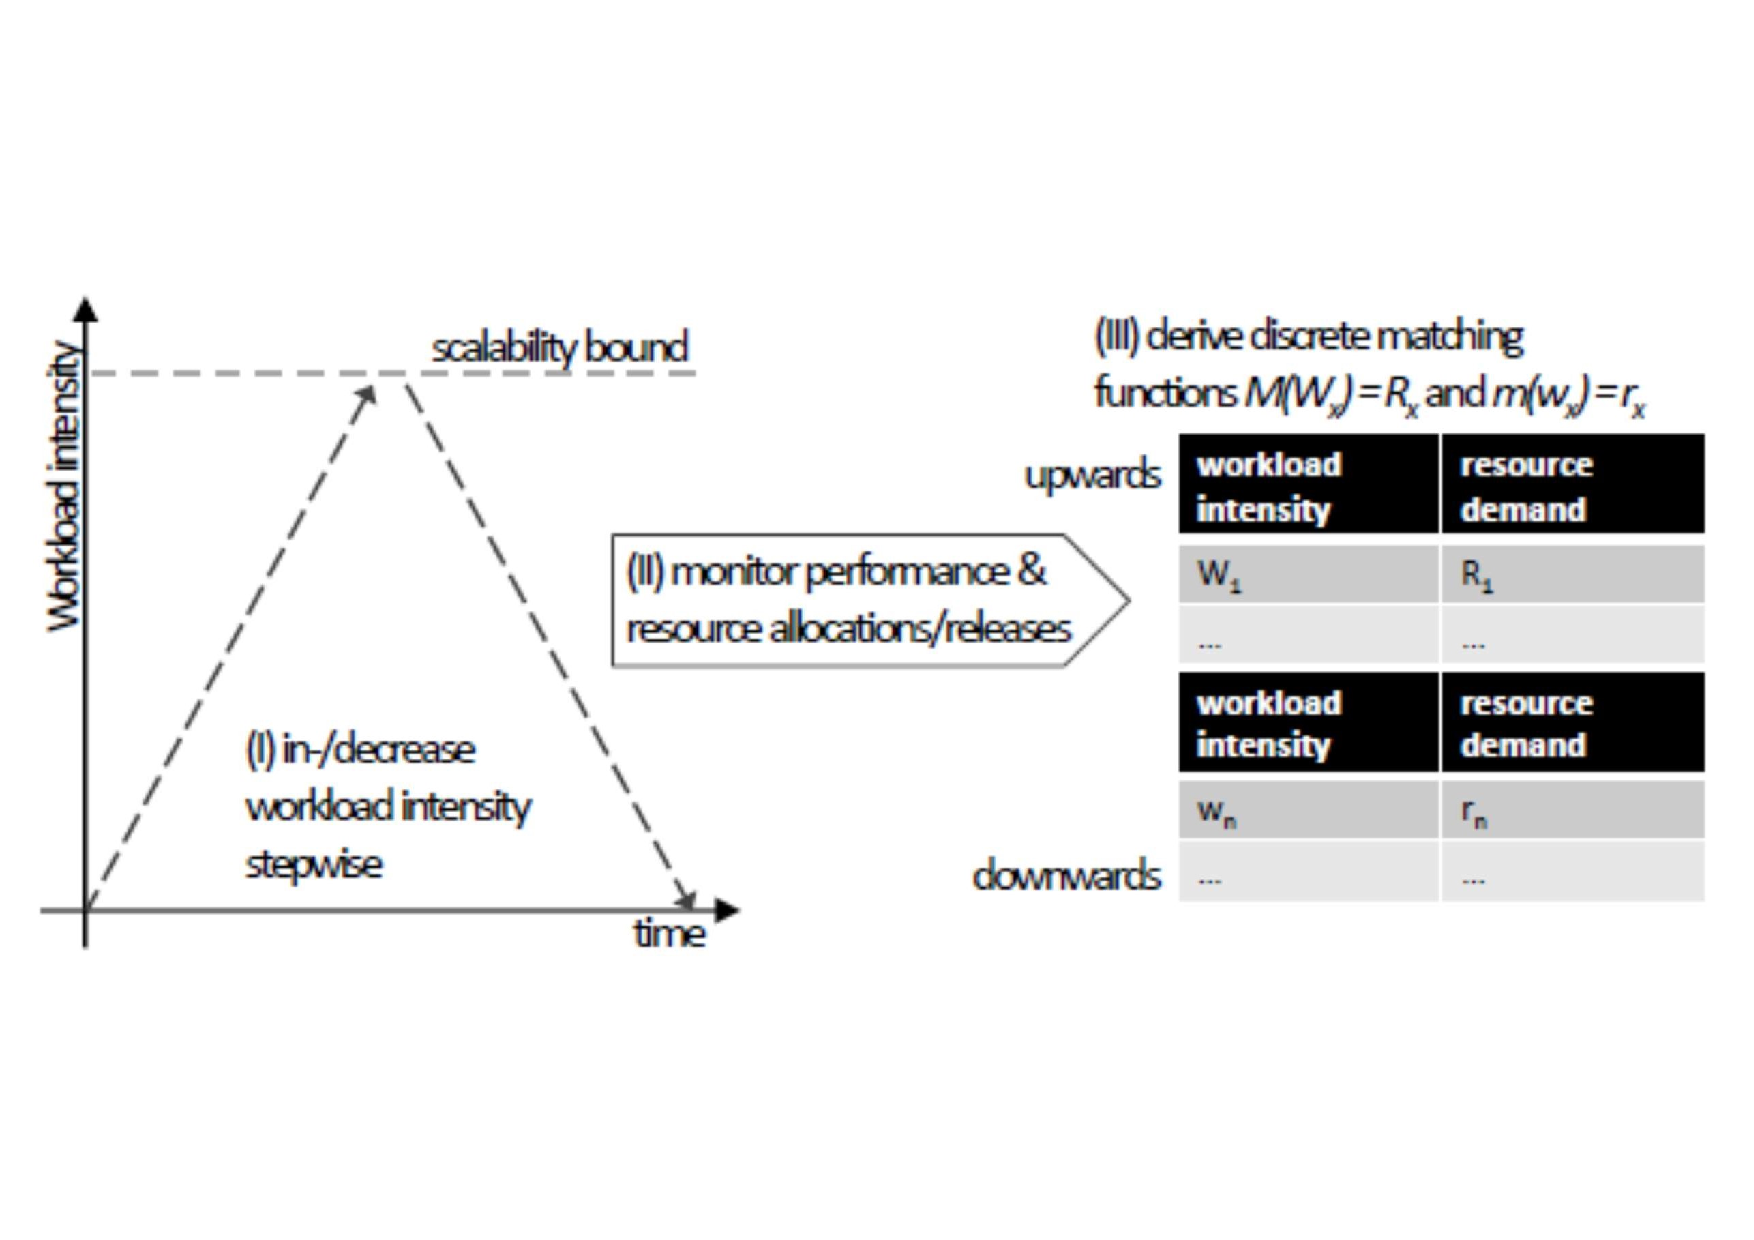
\includegraphics[width=\columnwidth]{Images/elasticity_matching_function.pdf}
	\vspace{-2.5cm}
	\caption[Elasticity Matching Function derivation.]{Elasticity Matching Function derivation.}
	\label{fig:elasticity_matching_function}
\end{figure}
\begin{figure}
	\vspace{-0.5cm}
	\centering
	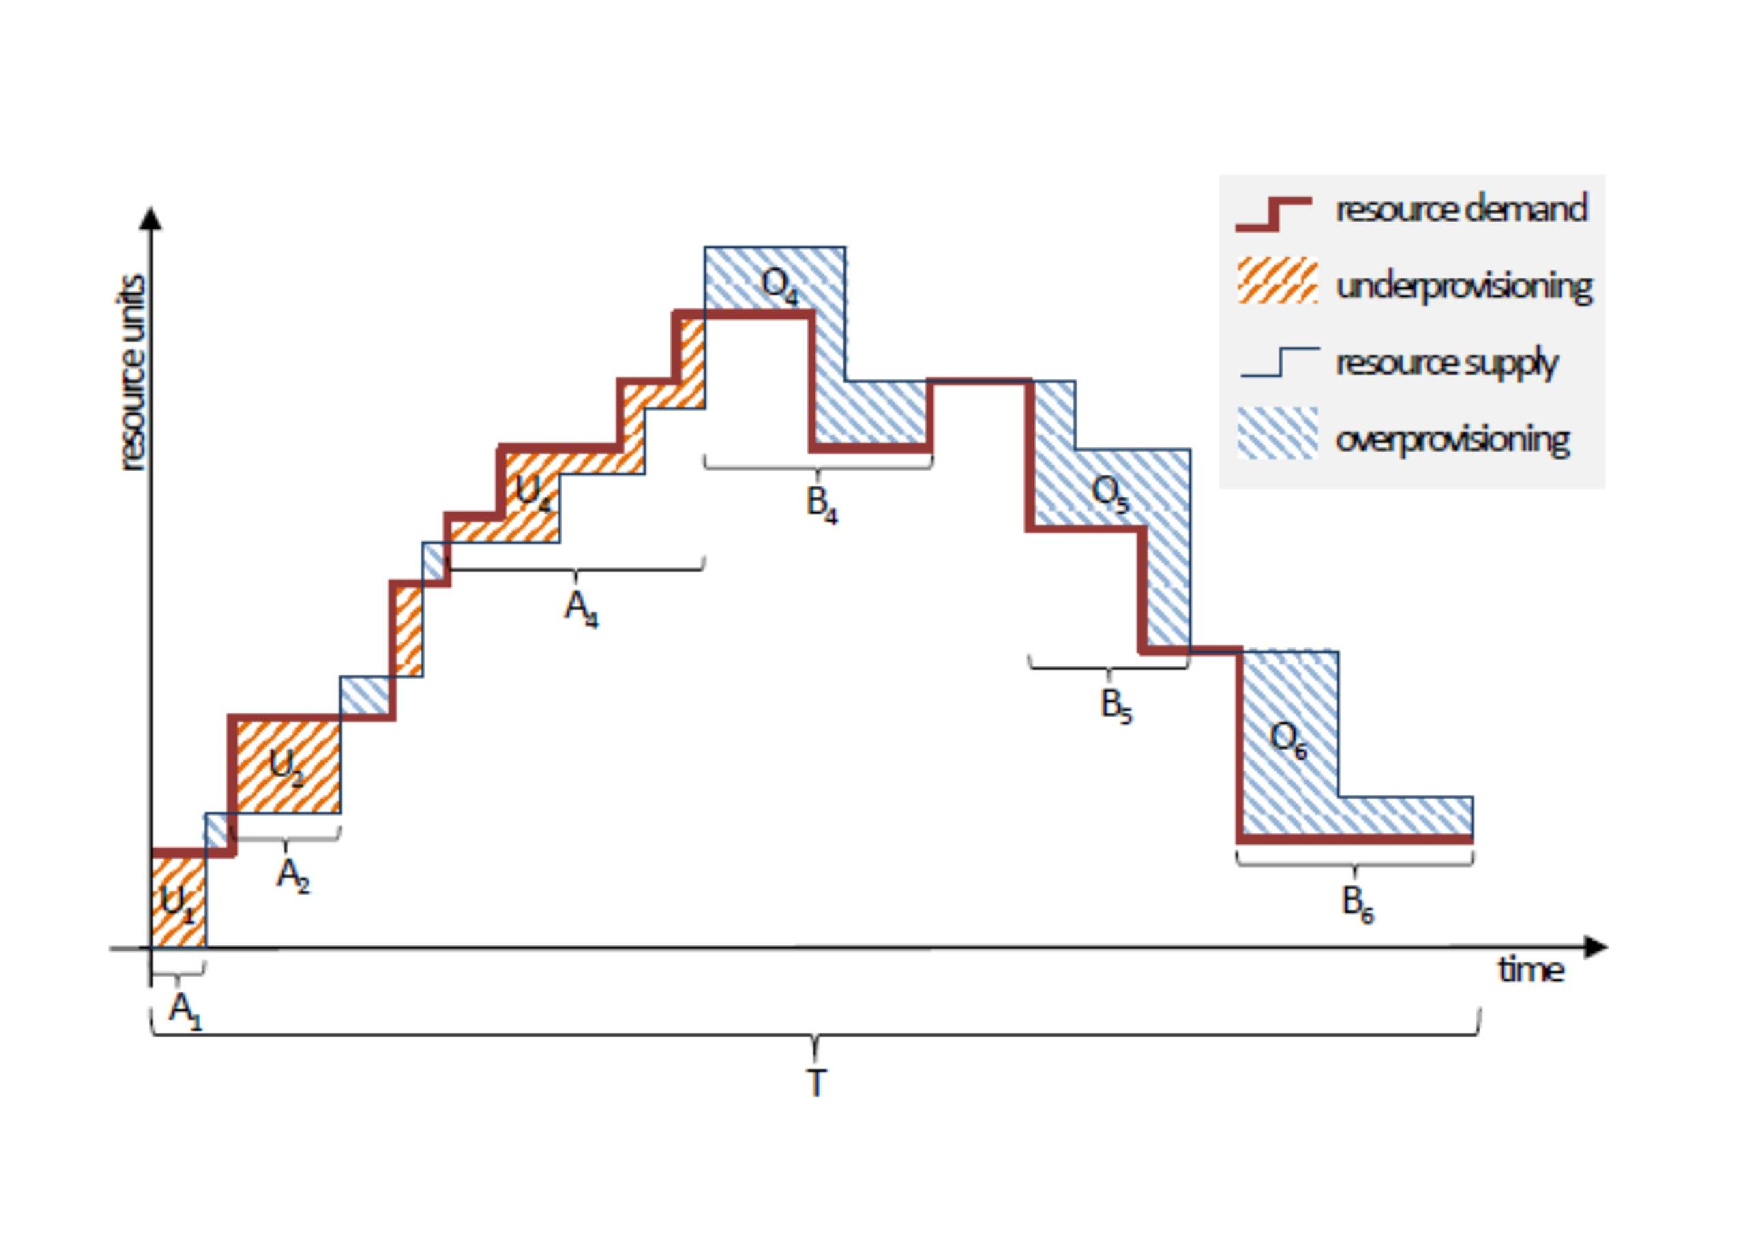
\includegraphics[width=\columnwidth]{Images/elasticity_resource_provisioning_chart.pdf}
	\vspace{-1.5cm}
	\caption[Resource Provisioning Chart.]{Resource Provisioning Chart.}
	\label{fig:elasticity_resource_provisioning_chart}
\end{figure}

Elasticity reflects the (theoretical) infinite upper bound on resource scalability in cloud computing and the frictionless resource renting model. Nevertheless elasticity is not just a synonym of resource management. Elasticity is also related to trade off between cost and quality~\cite{Dustdar2011}. Cost elasticity describes how resources are managed in response to cost changes, while quality elasticity measures how responsive is the quality to changes in resource utilization.

A \textit{matching function} $m(w) - r$ is a system specific function that gives the minimum quantity of resources r for any given resource type needed to meet the system’s performance requirements at a certain workload intensity. A matching function is required for both up and down scaling directions.

The matching functions can be determined based on measurements, as illustrated in \MyFig{fig:elasticity_matching_function}, by increasing the workload intensity w stepwise, and measuring the resource consumption r, while tracking resource allocation changes. The process is then repeated for decreasing w. After each change in the workload intensity, the system should be given enough time to adapt its resource allocations reaching a stable state for the respective workload intensity. As a rule of thumb, at least two times the technical resource provisioning time is recommended to use as a minimum. As a result of this step, a system specific table is derived that maps workload intensity levels to resource demands, and the other way round, for both scaling directions within the scaling bounds.

An example of how \textit{speed} and \textit{precision} affect resource provisioning is shown in \MyFig{fig:elasticity_resource_provisioning_chart}.


\section{Spark Resource Provisioning}\label{sec:spark_resource_provisioning}
Spark default deployment mode is standalone, that is using its embedded cluster manager. The cluster manager is responsible for starting the executor processes and set where and when they will run. Using the cluster manager embedded in Spark might be a problem in terms of resource utilization if we want to execute many concurrent distributed applications together with Spark. The use of a single cluster manager for different distributed applications gives a global view on the running applications and which ones are waiting to execute inside the cluster.

%It's important to recall that the cluster manager is responsible for starting executor processes and determine where and when they will run. Using Spark’s embedded cluster manager might be a problem in terms of resource utilization when we want to execute different distributed applications at the same time. Using a single cluster manager for different distributed applications has the advantage of providing a global view on which applications are running and which we want to execute inside the cluster.
Without a single cluster manager, there can be two main approaches to performing resource sharing and allocation:
\begin{itemize}
	\item  allow every application to allocate all the resources in the cluster at the same time: this leads to an unfair situation of resource contention
	\item split the resource pool into smaller ones, one per application.
\end{itemize}
With the second approach resource contention are avoided, at the cost of a less efficient utilization of the resources, as some of the applications might request more resources than the ones assigned to their pool, while some others might end up using less resources than the one they have access to.
A dynamic approach to resource allocation leads to a better resource utilization. Spark natively supports the execution on top of Apache Hadoop YARN and Apache Mesos cluster managers.
Spark supports the dynamic allocation of executors, also known as elastic scaling. This feature allows addition and removal of Spark executors dynamically to follow the workload demand.
In traditional static allocation, a Spark application would allocate CPU and memory upon application start, not caring about the level of resources effectively used later on. Dynamic allocation instead allows the allocation of as much resources as they are necessary, thus avoiding to waste them. The number of running executors follows the workload, in particular
idle executors are removed and re-launched when there are tasks waiting 
to be executed. Dynamic allocation can be activated in Spark settings and should be used in conjunction with the External Shuffle Service.  Doing so, data that have been manipulated
by an executor will still be available after the executor is removed. 
Dynamic allocation has two different policy for scaling the executors:
\begin{itemize}
	\item Scale Up Policy: new executors are requested when there are pending tasks. There is an exponential increase in the number of executors, because the start is conservative, so at the end the application might need a higher number of them
	\item Scale Down Policy: idle executors are removed after a certain amount of time, and this amount of time is configurable
\end{itemize}
In order for dynamic allocation to work, it must be configured the initial number of executors that are created when application starts, and the minimum and maximum number of executors that can be reached when scaling down and up respectively. Dynamic allocation is available on all cluster managers currently supported by Spark, including Standalone mode.

\subsection{Apache Hadoop Yarn}\label{sec:hadoop_yarn}
Apache Hadoop YARN (acronym of Yet Another Resource Negotiator) is an evolution of the Hadoop computing  platform ~\cite{Vavilapalli:2013:AHY:2523616.2523633}. 
\begin{figure}
	\vspace{-1.5cm}
	\centering
	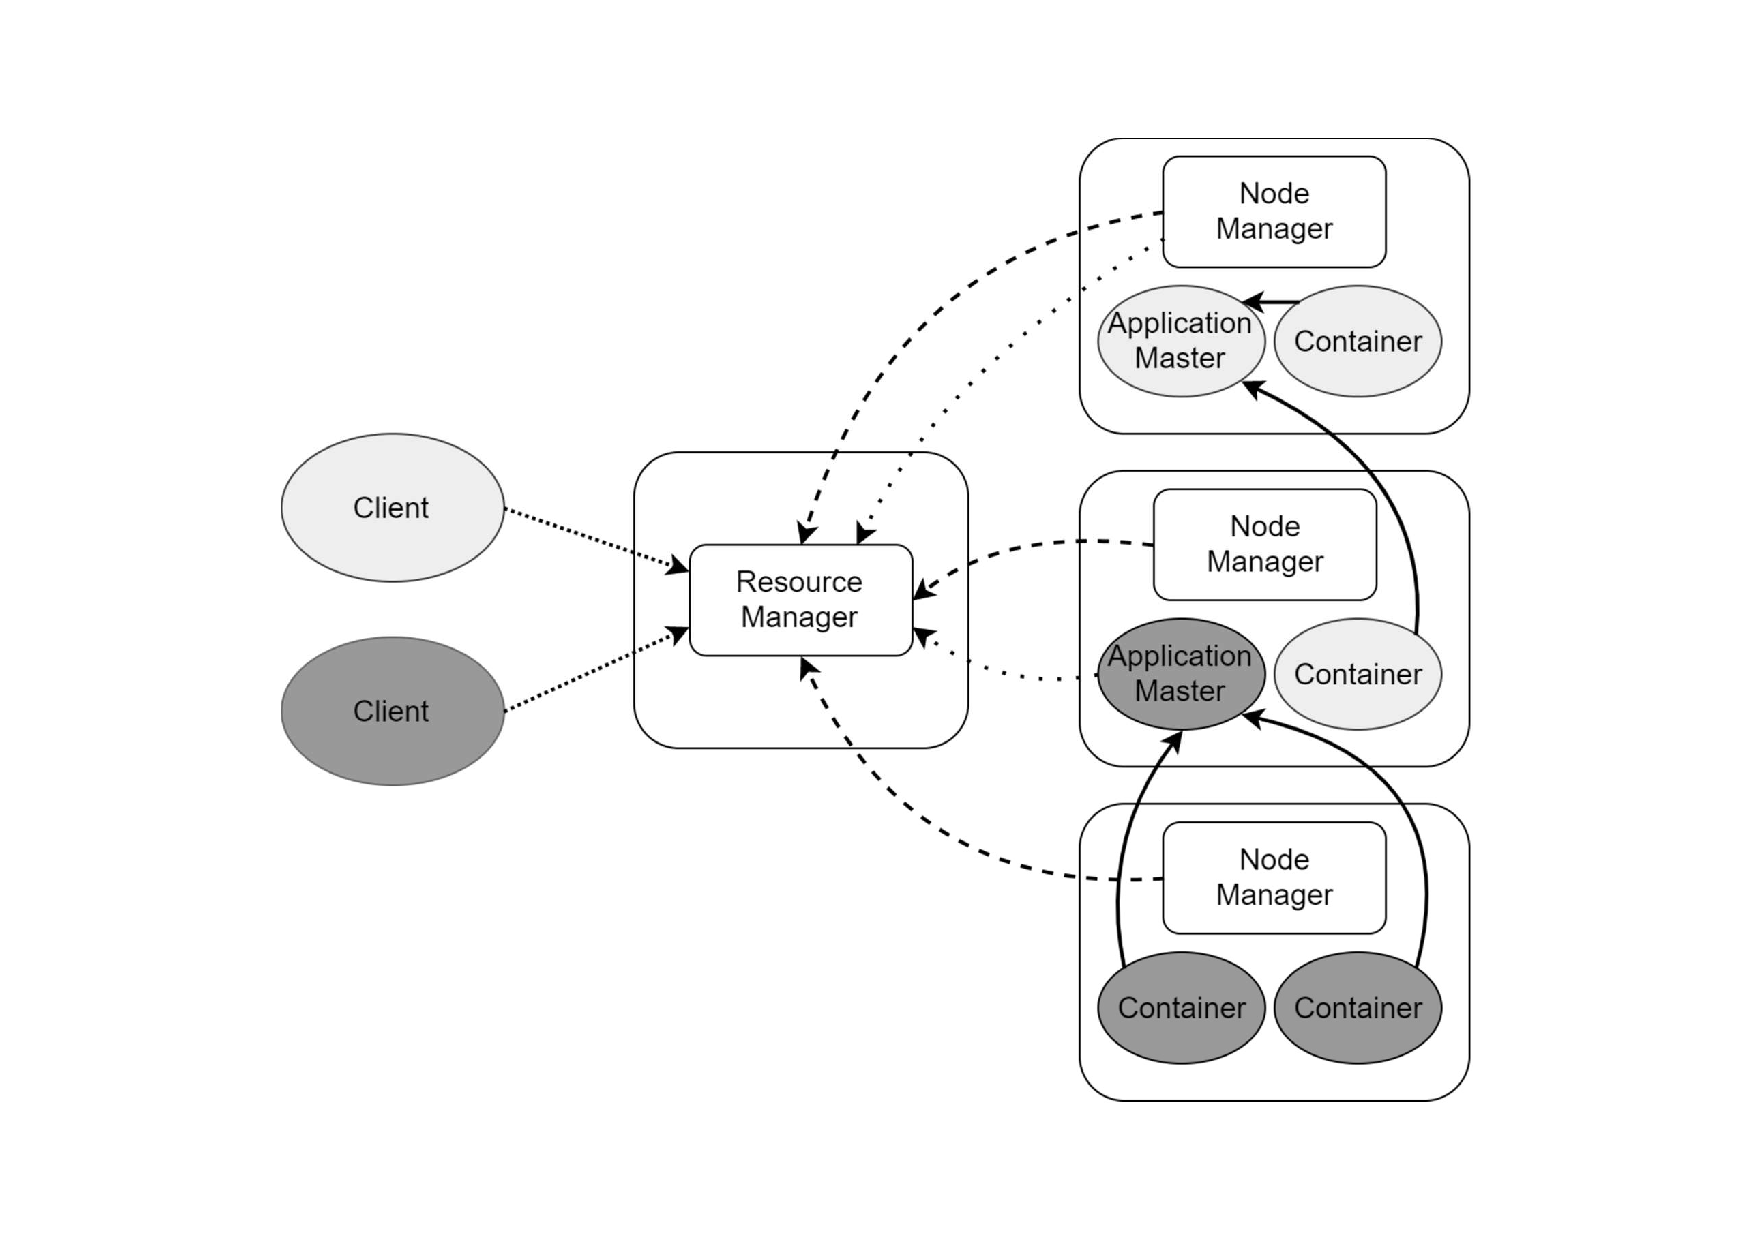
\includegraphics[width=\columnwidth]{Images/apache_hadoop_yarn_architecture.pdf}  
	\vspace{-1.5cm}
	\caption[Apache Hadoop YARN Architecture]{Apache Hadoop YARN Architecture.}
	\label{fig:apacheHadoopYarnArchitecture}
\end{figure}
It separates the functionality of resource management from job scheduling and monitoring. This is done by starting two different types of daemons: a global Resource Manager (RM) and a per-application Application Master (AM). 

The data computation framework is made by Resource Manager (RM) and Node Manager (NM) (see \MyFig{fig:apacheHadoopYarnArchitecture}). Resources among all the applications that are running in the system are managed by RM authority, while NM is the per-machine daemon who manages containers, monitoring and reporting. The per application AM negotiates resources with RM and works with NM  to execute and monitor tasks. Resource Manager (RM) is composed by Scheduler and Applications Manager. 

%The Scheduler allocates resources to the running applications considering constraints about capacity, queues, etc. It is a pure scheduler, as it does not monitor neither tracks any application, and it does not guarantee that a failed application will be restarted after an application or hardware failure. It allocates resources upon applications' request. It materializes  the abstract notion of container which has elements as memory, CPU cores, disk and network bandwidth. Pluggable policies determine the re-partition of resources among the different applications, for example the Capacity Scheduler, designed for multi-tenant clusters, and the Fair Scheduler, that shares cluster resources fairly. 

%The Applications Manager accepts the jobs submissions, negotiates the first container that will execute the AM and exposes a service that can restart the AM in case of failure. The per-application AM negotiates the containers needed from the Scheduler, track their status and monitor their progress. The RM keeps a global model of the cluster state and uses the resource requirements reported by the running applications to enforce a global scheduling. The RM generates containers along with tokens that grant access to resources in response to AM requests. The applications can be requested to return the resources back to the RM, for example when cluster resources become scarce. This feature is an extension of the protocol.

%The execution of an application inside the cluster is coordinated by the  Application Master (AM) process. The AM itself runs in the cluster, just like any other container. Heartbeats are periodically sent by the application to the RM as a mechanism to confirm its liveliness and to update the Scheduler about its resource requests. After having modeled the application requirements, the AM encodes its preferences and constraints inside the heartbeat message. This information is stored in the form of Resource Request, specifying the desired number of containers (e.g., 10 container), the resources of each container (e.g., <3 CPU, 4 GB>), the preferred locality and the priority of the request priority in the context of the application. Upon receipt of container lease, the AM can modify its execution plan to take into account the abundance or scarcity of the resources. The YARN worker daemon is called Node Manager (NM), that is in charge of authenticating container lease, managing dependencies, monitoring the execution of containers and offering them a set of services. After having registered with the RM, the NM sends heartbeats to communicate its status and receives instructions from the RM. Containers are described by a container launch context (CLC), that keeps track of all the environment variables, their dependencies and the security tokens. It also takes care of the payloads and the commands needed by NM services to launch the process inside the container. After a container lease authenticity validation, the NM configures the container with the specified resource constraints and initializes a monitoring subsystem. Dependencies are copied into local storage in order to launch the container. NM can also kill containers upon RM or AM request, for example when a tenant is removed or when an application completes. When a container exits, NM cleans its working directory. When an application ends, all the resources held by its container on all nodes are released. A periodic healthy check is made by NM periodically checks the state of the physical machine and informs the RM of a possible unhealthy state.

\subsection{Apache Mesos}\label{sec:apache_mesos}
Apache Mesos~\cite{Mesos} is an open-source project used to manage computer
clusters. 
\begin{figure}
	\vspace{-1cm}
	\centering
	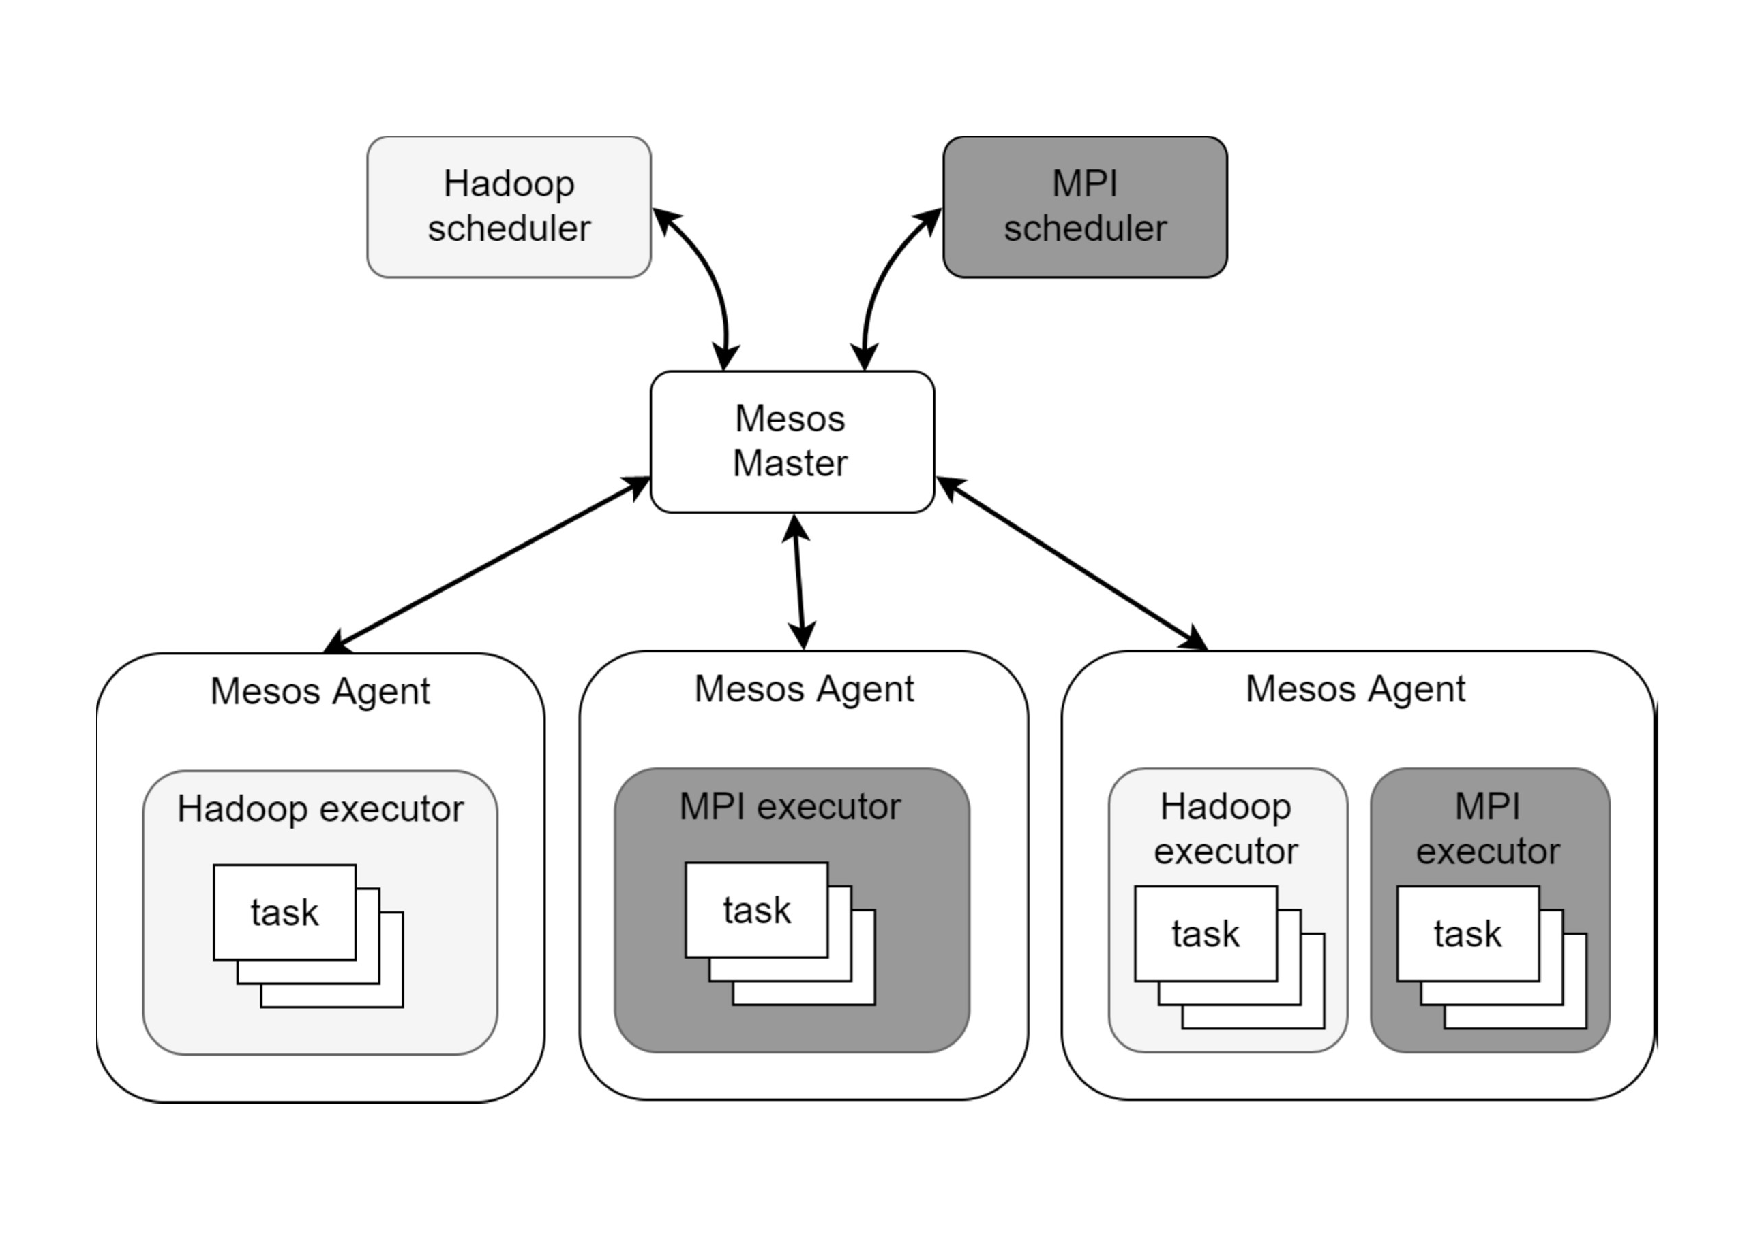
\includegraphics[width=\columnwidth]{Images/apache_mesos_architecture.pdf}  
	\vspace{-1cm}
	\caption[Apache Mesos Architecture]{Apache Mesos Architecture.}
	\label{fig:apacheMesosArchitecture}
\end{figure}
The purpose of Mesos is to share cluster between different computing frameworks, such as Apache Hadoop or Message Passing Interface (MPI)~\MyFig{fig:apacheMesosArchitecture}. The sharing increments the utilization of the cluster
and prevents per-framework data replication. 
Mesos shares resources in a fine-grained way, allowing to achieve data locality. It presents a scheduling mechanism on two layer called resource offers. Mesos decides how many resources to offer to each of the running frameworks, meanwhile they decide how many resources to accept and which computation to execute on the granted resources. 

%New cluster computing frameworks continue to emerge, it is clear that finding a framework that is optimal for all type of application is almost impossible. We expect that organization would like to use different frameworks inside the same cluster, picking the best one according to the kind of application that they are going to execute. Two classic solution are: i) statically partitioning the cluster and executing one framework per partition; ii) allocate a set of VMs to each of the frameworks. Unluckily these solution do not achieve high utilization and efficient data sharing. The main problem is the different allocation granularity of these solutions and the one of the existing frameworks, for example Hadoop employs a fine grained resource sharing model, where nodes are divided into slots and each job is composed by short tasks that match the slots.
\begin{figure}[t]
	\vspace{-1.5cm}
	\centering
	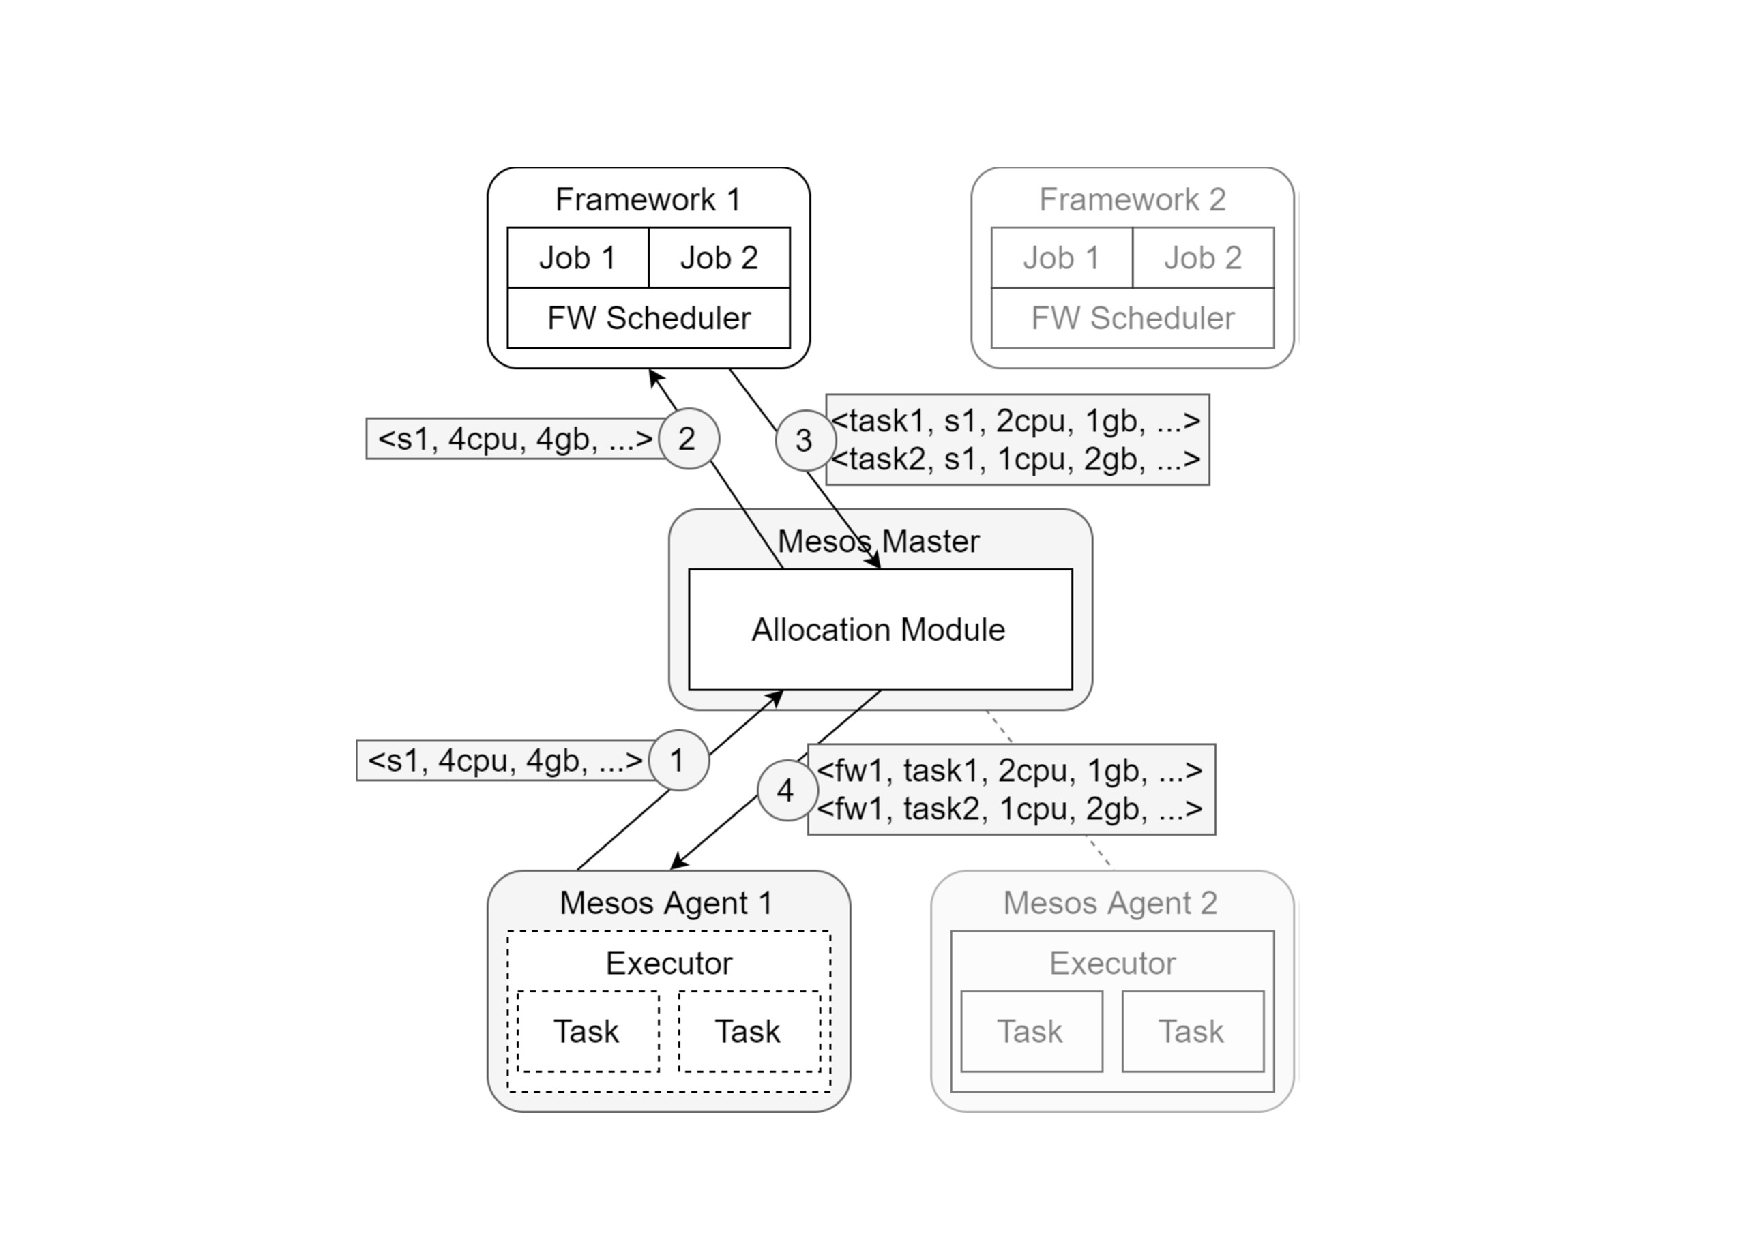
\includegraphics[width=\columnwidth]{Images/apache_mesos_resource_offer_example.pdf}  
	\vspace{-1cm}
	\caption[Apache Mesos Resource Offer Example]{Apache Mesos Resource Offer example. 1) Mesos Agent 1 reports
		free resources to the Allocation Module; 2) Allocation
		Module offers resources to Framework 1 scheduler; 3) Framework
		1 scheduler accepts resources and assign tasks; 4) Allocation
		Module launches tasks on the executor running in Mesos
		Agent 1.}
	\label{fig:apacheMesosResourceOfferExample}
\end{figure}
%The presence of short tasks allows us to achieve high utilization, as jobs can rapidly scale when new nodes are available. But it is not possible to achieve fine grained sharing across frameworks, because they have been developed in an independent way, and thus it is difficult to efficiently share the cluster among different frameworks.

%Mesos delegates the control over the scheduling to the different frameworks. In this way it is possible to have the abstraction of the resource offers, that encapsulate a bundle of resources that the framework can allocate on a node in order to execute a task. Mesos decides how many resources to offer to each framework, this is based on policies, and the framework decides which resources to accept and which tasks to execute on them. Even though this approach does not lead to a globally optimum scheduling, it has been proved that it performs particularly well in practice, allowing the frameworks to obtain near perfect data locality. Mesos provides other benefits to its users, for example the possibility of running different instances of the same framework or even different versions.

%Mesos is composed by a master process that manages slave daemons running on each cluster node and frameworks that run tasks on these slaves, as we can see from  \myFig{fig:apacheMesosArchitecture}. Master implements fine-grained sharing across frameworks using resource offers. Every resource offer is a list of free resources on the different slave nodes. The master decides how many resources to offer to each framework, according to some policy such as fairness or priority. Every framework that is running on Mesos is composed by two components: a scheduler, that registers with the master in order to obtain the resource offers, and an executor process that is launched on the slave node in order to execute framework’s tasks. While the master chooses how many resources to offer, the scheduler chooses which resources to use among those offered. When an offer is accepted, the scheduler sends to the master the description of the tasks that should be executed. The resource offer process is repeated every time tasks are finished and when there are new free resources. In order to maintain a light interface, Mesos does not ask the frameworks to specify their resource requirements or constraint, instead it gives them the possibility of refusing offered resources. Mesos allows frameworks to set up a set of filters, in the form of boolean predicates, specifying the conditions on which the framework will always refuse a proposal (e.g., providing a whitelist of nodes it can run on). In  \MyFig{fig:apacheMesosResourceOfferExample} we have an example of resource offer process.

%Resource allocation is performed by a pluggable allocation module, such that it is possible to meet different organization needs. The two basic allocation modules are fair sharing and strict priorities, similar to those available on Apache Hadoop. In the normal situation, Mesos %does exploits the fact that the majority of the tasks are short and so it reallocates resources only when tasks end. This usually happens frequently and so a new launched framework can obtain its share quickly. The allocation module can also revoke tasks, killing them, but before doing so it concedes a grace period to the framework in order to terminate them properly. The allocation module chooses the policy to revoke tasks, it needs to take into account the fact that this might be of little impact on some framework (e.g., MapReduce), but it can be critical in frameworks that have interdependent tasks (e.g., MPI). For this reason, the allocation module exposes a guaranteed allocation for each of the frameworks, an amount of resources that the framework can allocate without the risk of losing tasks, this value can be retrieved by the framework using an API call. If the framework total allocation is under the guaranteed one, it has no risk of seeing its task killed, on the other hand instead, if the allocation is over the guaranteed one, any of its tasks can be terminated.

%Performance isolation between frameworks executor running in the same slave is achieved by leveraging existing OS isolation mechanism. Since they are platform dependent, pluggable isolation modules are supported.

\subsection{Spark on Yarn}\label{subsec:sparkOnYarn}
Support for running Spark on YARN was added to Spark in version 0.6.0 and has been improved in subsequent releases~\cite{misc:SparkOnYarn}.

When running on YARN, each Spark executor is run inside a YARN container. Spark supports two different modes to run on YARN, the Yarn-cluster and Yarn-client mode.

In client mode, as shown in \myFig{fig:sparkOnYarnClientMode}, the driver program is run inside the client process. In this way, the Application Master (AM) that is run in a YARN container is used only to request resources to the Resource Manager (RM). This mode is useful for interactive applications and for debugging purposes, since you can see application output
immediately on the client side process. If the client disconnects from the cluster, the Spark application will terminate, this is due to the fact that the driver process resides on the client.

In cluster mode instead, as shown in \MyFig{fig:sparkOnYarnClusterMode}, Spark driver program is run inside the AM process managed by YARN. After initializing the application, client can disconnect from the cluster and reconnect later on. This mode makes sense when using Spark on YARN in production jobs. 

Running on top of YARN cluster manager has some benefits. First
of all YARN allows to dynamically share the cluster resources between the different frameworks that are running together. For example we can run MapReduce jobs after running Spark jobs without the need of changing YARN configurations. Moreover, YARN supports for categorizing, isolating and prioritizing workloads and employs security policies, in this way Spark can use secure authentication between its processes.
\begin{figure}
	\vspace{-1cm}
	\centering
	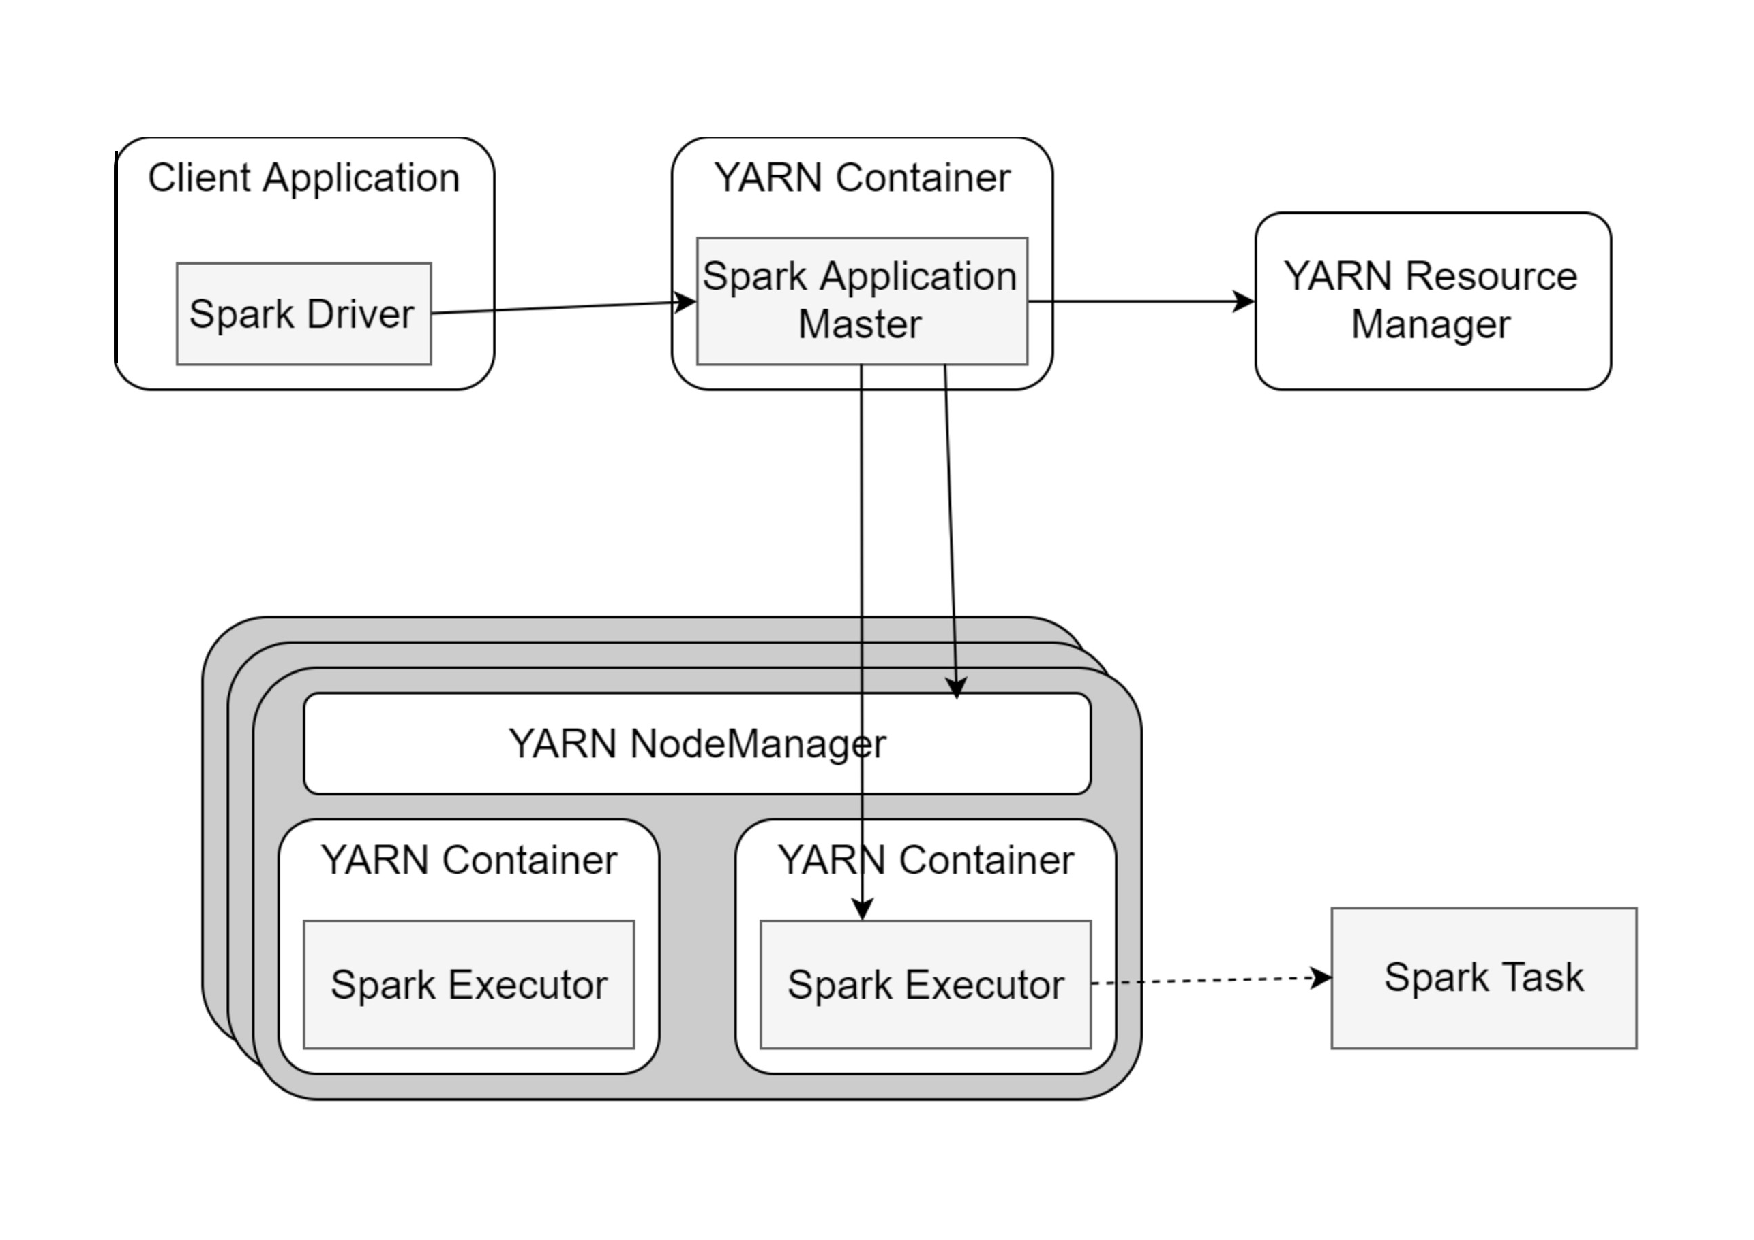
\includegraphics[width=\columnwidth]{Images/spark_yarn_client_mode.pdf}  
	\vspace{-1cm}
	\caption[Spark on YARN Client Mode]{Spark on YARN Client Mode.}
	\label{fig:sparkOnYarnClientMode}
\end{figure}
\begin{figure}
	\vspace{-1cm}
	\centering
	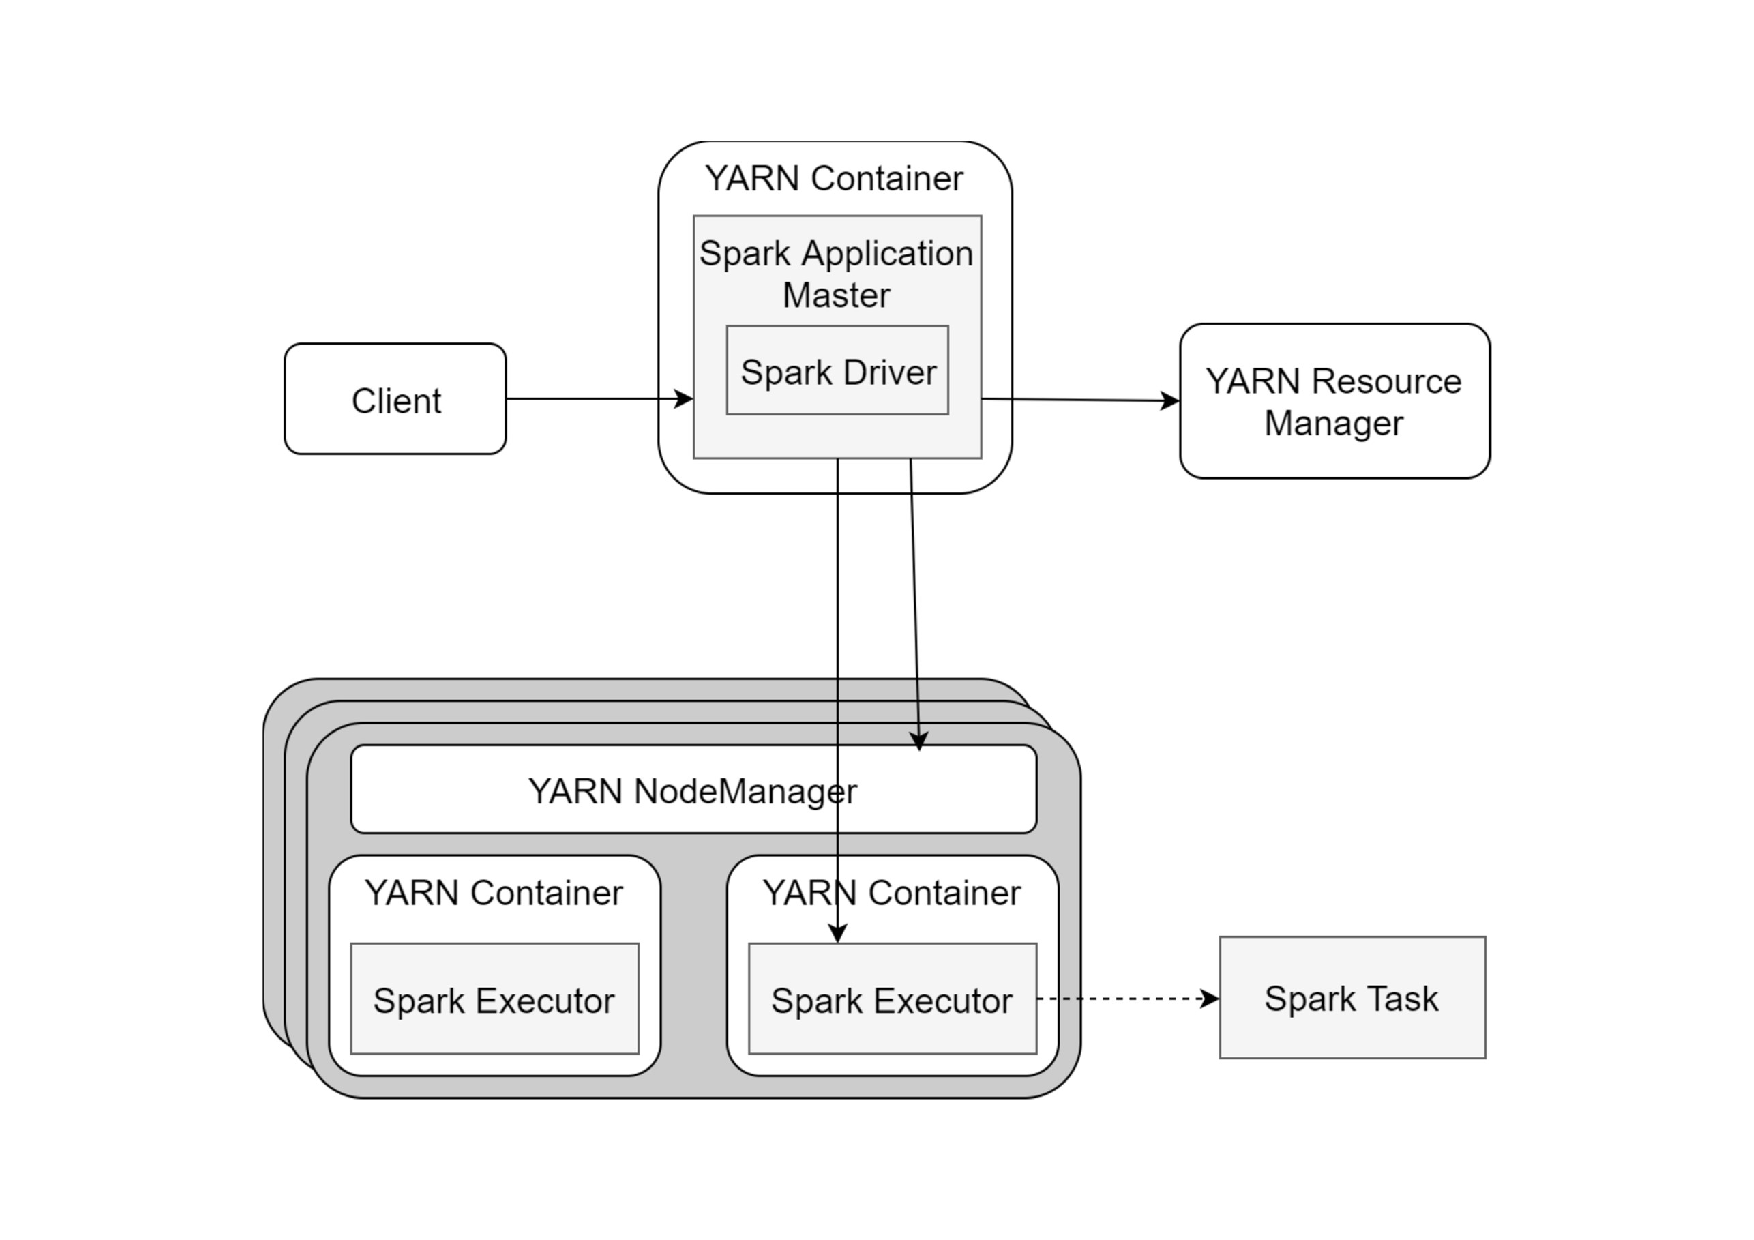
\includegraphics[width=\columnwidth]{Images/spark_yarn_cluster_mode.pdf}  
	\vspace{-1cm}
	\caption[Spark on YARN Cluster Mode]{Spark on YARN Cluster Mode.}
	\label{fig:sparkOnYarnClusterMode}
\end{figure}

When running on YARN, Spark executors and driver program use
about 6-10\% more memory with respect to the standalone execution,
this is due to the fact that this extra amount of off-heap memory is
allocated in order to take into account YARN overheads.

\subsection{Spark on Mesos}\label{subsec:sparkOnMesos}
Support for running Spark on Mesos was added to Spark in version 1.5. Spark on Mesos can be executed in two different modes: coarse-grained and fine-grained \cite{misc:SparkOnMesos}.
In coarse-grained mode, as shown in \myFig{fig:sparkOnMesosCoarseGrainedMode}, each Spark application is submitted to Mesos master as a framework and Mesos slaves will run tasks for the Spark framework that are Spark executors. Mesos tasks are launched for each Spark executor and those Mesos tasks stay alive during the lifetime of the application unless we are using dynamic allocation or the executor is killed for various reasons. The advantage of coarse-grained mode is in a much lower task startup overhead, with respect to the other mode, and so it is good
for interactive sessions.

The drawback is that we are reserving Mesos resources for the complete duration of the application, unless dynamic allocation is active. Dynamic allocation allows to add and remove executors based on load: i) kill executor when they are idle, ii) add executors when tasks
queue up in the scheduler. To use dynamic allocation it is required that the external shuffle service is running on each node.

In fine-grained mode, shown in \myFig{fig:sparkOnMesosFineGrainedMode}, Mesos tasks are launched for each Spark task, and those tasks die as soon as Spark tasks are done. This mode has too much overhead in case that Spark has too many tasks, for example if Spark application has 10,000 tasks, then Spark needs to be installed 10,000 times on Mesos agents. Because
of this huge overhead, fine-grained mode has been deprecated since Spark version 2.0.0.         This mode allows multiple instances of Spark to share cores at a very fine granularity, but it comes with an additional  overhead in launching each task. Thus this mode is inappropriate
for low-latency requirements like interactive queries or serving web requests, instead it is fine for batch and relatively static streaming. 

Similarly to what happens on YARN, it is possible to run spark in Mesos-client or Mesos-cluster mode. In client mode, the driver process
is executed in the client machine that submits the job, so it is required that it stays connected to the cluster for the entire time of the application execution. In cluster mode instead, the driver program is run on a machine of the cluster.
\begin{figure}
	\vspace{-1cm}
	\centering
	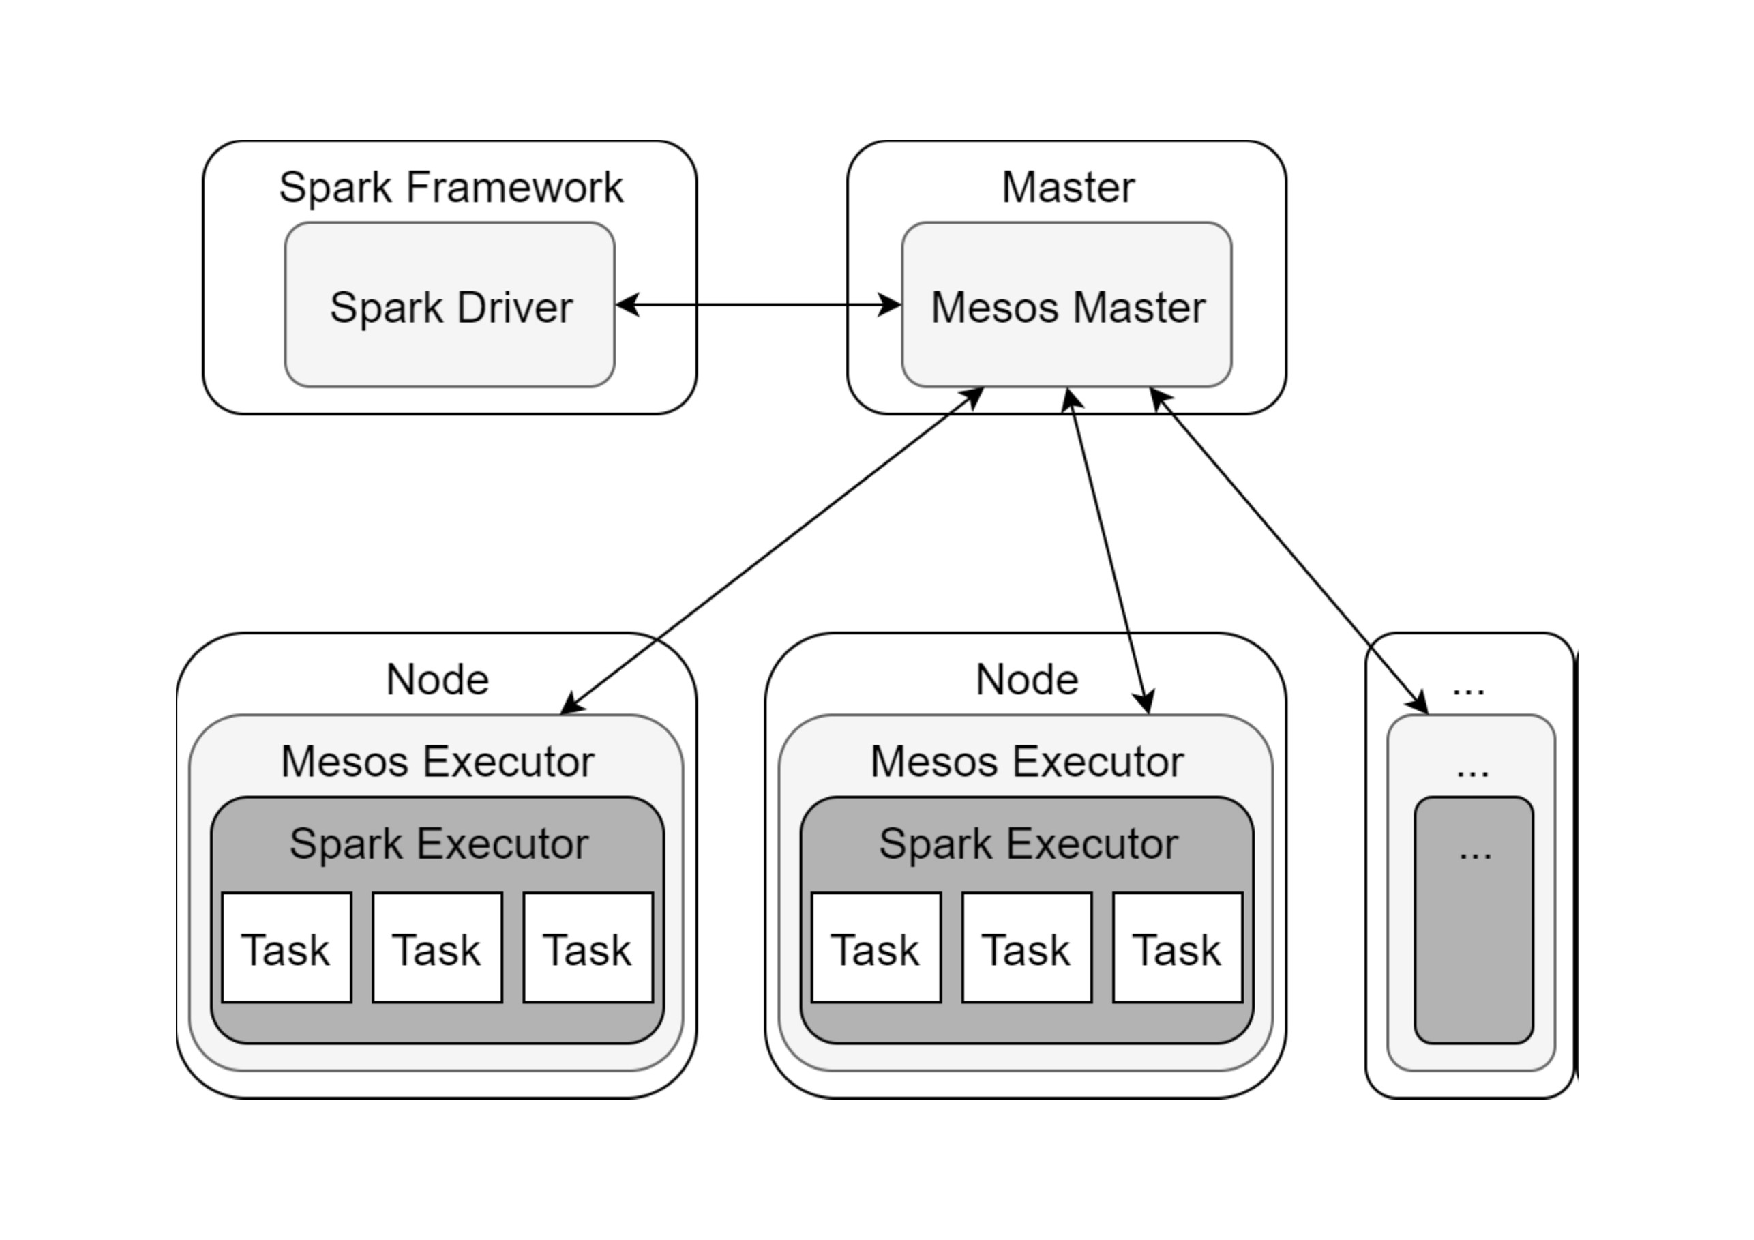
\includegraphics[width=\columnwidth]{Images/spark_mesos_coarse_grained_mode.pdf}  
	\vspace{-1cm}
	\caption[Spark on Mesos Coarse Grained Mode]{Spark on Mesos Coarse Grained Mode.}
	\label{fig:sparkOnMesosCoarseGrainedMode}
\end{figure}
\begin{figure}
	\vspace{-1cm}
	\centering
	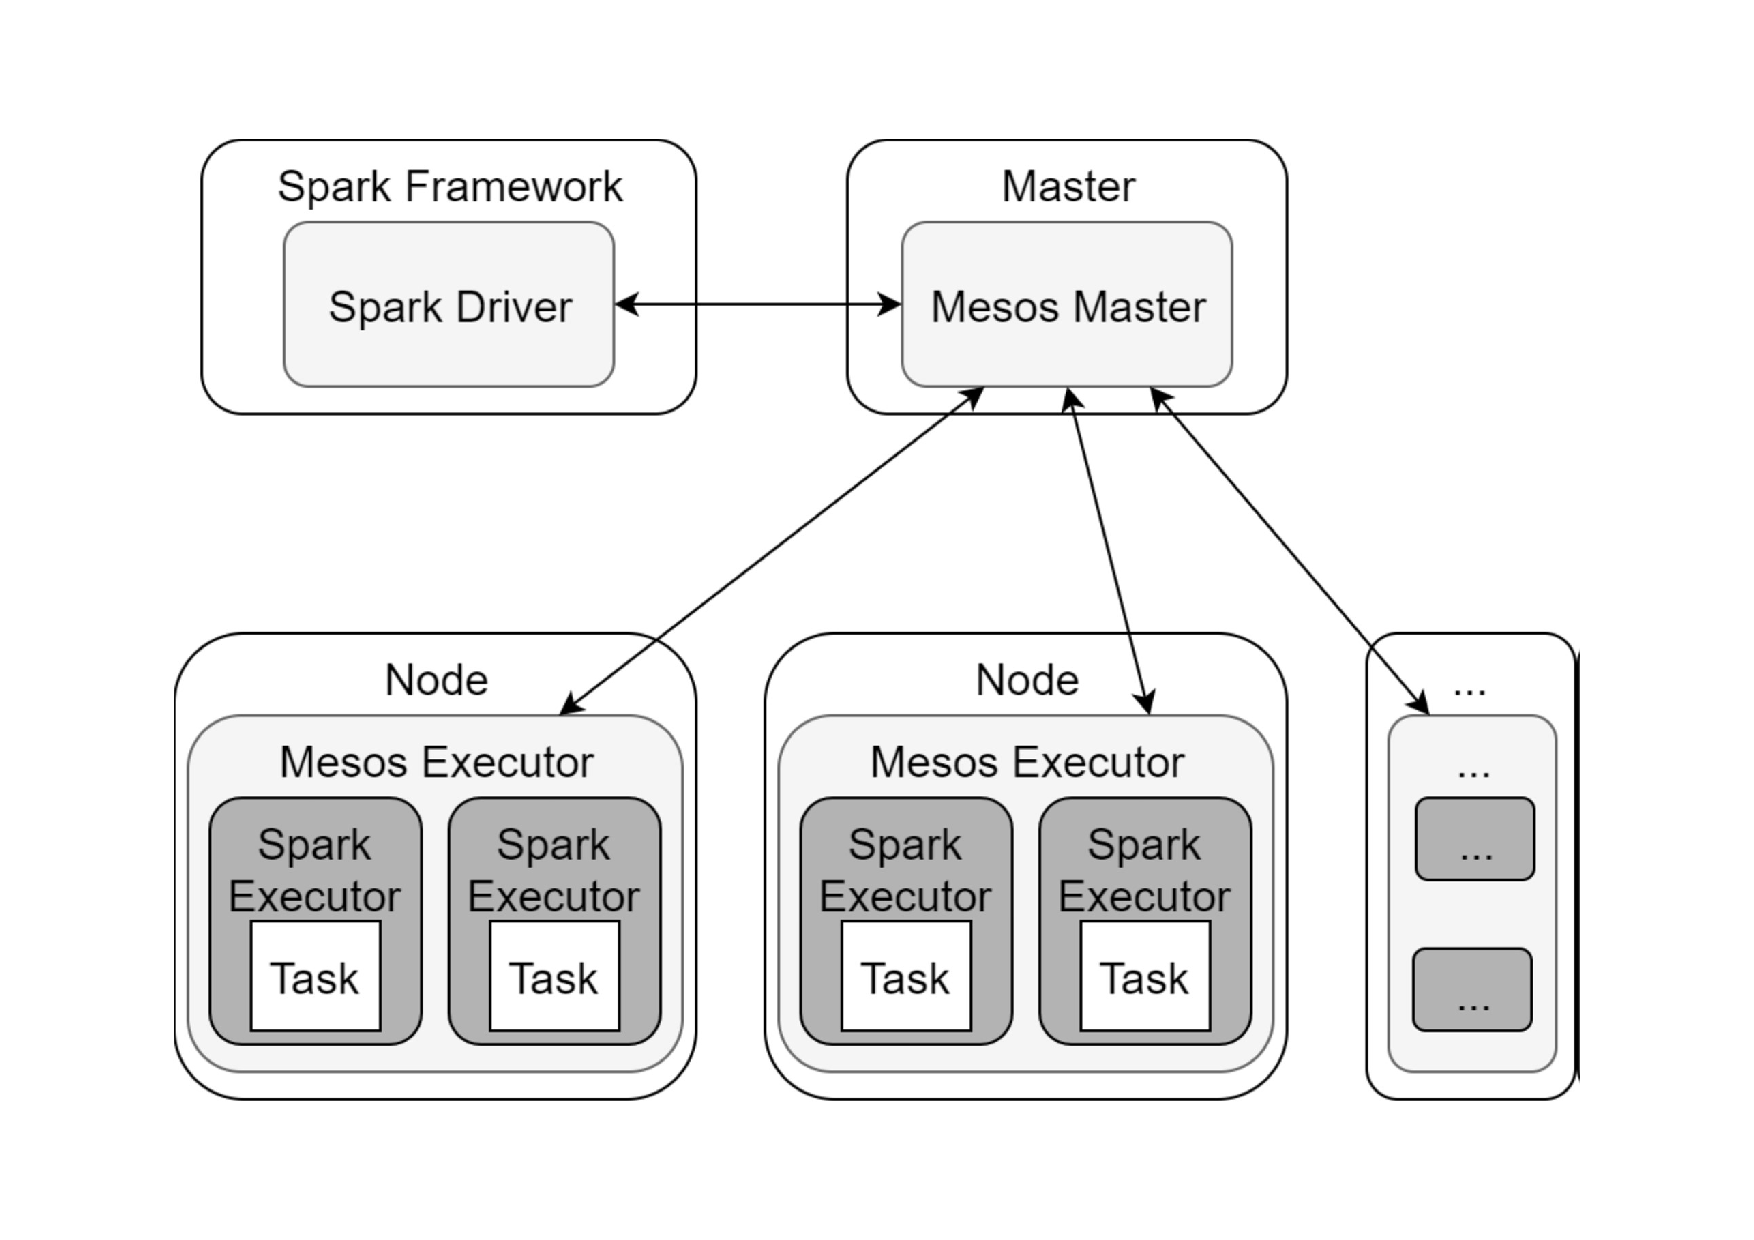
\includegraphics[width=\columnwidth]{Images/spark_mesos_fine_grained_mode.pdf}  
	\vspace{-1cm}
	\caption[Spark on Mesos Fine Grained Mode]{Spark on Mesos Fine Grained Mode.}
	\label{fig:sparkOnMesosFineGrainedMode}
\end{figure}

%\section{Virtualization and Containerization}
%Virtualization refers to creating the virtual version of something, included hardware components, storage devices and computer networks.
%Virtualization is born in 1960's, as a way to logically partition the system resources offered by a mainframe computer between many different applications. From this point, the meaning of the word has been widely extended.

%Virtualization is a technology that allows creating multiple simulated environments or dedicated resources from a single unique physical hardware system. An hypervisor is a software that can directly connect to the hardware, with the purpose of splitting the unique physical system into separated environments, different from each other and secure, known as virtual machines (VM's). These VM's rely on the hypervisor ability to separate the hardware resources and distribute them in a proper way. The original physical machine equipped with the hypervisor is called host, meanwhile the VM's are called guests. These guests use the computation  resources, such as CPU, memory and storage, as a set of resources that are easily re-allocatable. The operators can control the virtual instances of CPU, memory, storage and other resources, so that the guests can receive all the resources they need to execute their task. The words host and guest are used to distinguish the software that runs on the physical hardware from the software that is running on the virtual machines.

%Hardware virtualization or platform virtualization refer to the creation of a VM that acts like a real computer with an OS. The software that is run in this VM is separated from the underlying hardware.
%This allows us to run particular configurations, for example we run a computer with a Windows OS that hosts a VM with Linux as guest OS.

%There are at least two different hardware virtualization types:
%\begin{itemize}
%	\item full virtualization: it completely simulates the hardware in order to allow the software, typically a guest OS, to be run without the need of modifications
%	\item paravirtualization: the hardware environment is not simulated, anyway guest programs are run in isolated domains, as if they were run in completely separated systems. Guest programs need to be modified in a specified way in order to run in this kind of environment.
%\end{itemize}
%\begin{figure}
%	\centering
%	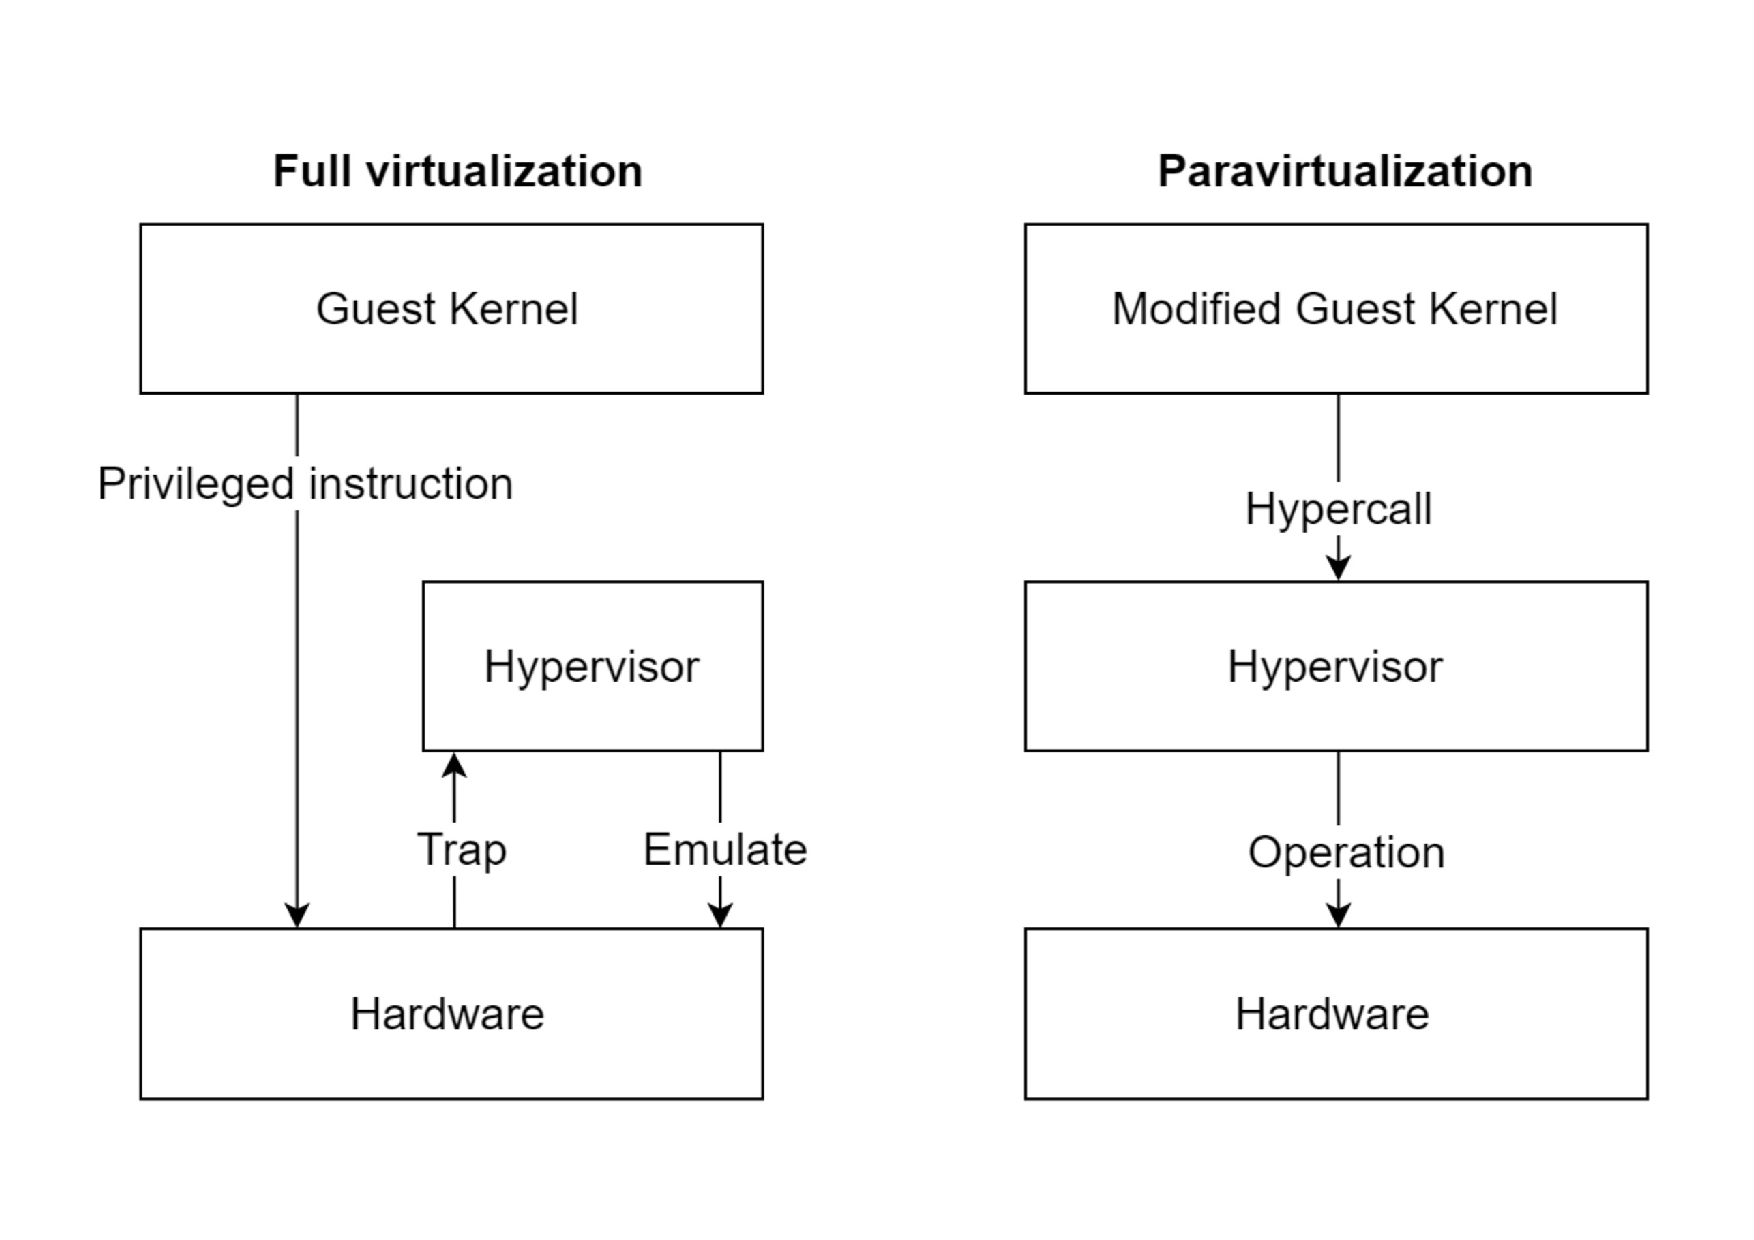
\includegraphics[width=\columnwidth]{Images/virtualization_paravirtualization.pdf}  
%	\caption[Full virtualization and paravirtualization]{Full virtualization and paravirtualization.}
%	\label{fig:virtualizationParavirtualization}
%\end{figure}

%In \myFig{fig:virtualizationParavirtualization}, we can see the differences between the two kind of virtualization. In paravirtualization, the VM presents a different interface compared to the one of a physical machine. This requires modification in the guest OS in order to allow its execution inside the VM. The hypervisor exposes a set of APIs that the guest OS must use to execute privileged instructions. Calls to these particular functions are often defined as Hypercalls. In full virtualization instead, VM have the same interface as the physical ones. Ideally, the guest OS would not be able to determine if it is being run on a physical or virtual machine. The great advantage of full virtualization is that we do not need to modify the OS. In this way the hypervisor can adopt a trap system to execute privileged instructions. 

%We can improve the efficiency of the virtualization by using hardware assisted virtualization, in particular we can decide to use CPU's that provide efficient support for virtualizing on hardware, but also other kind of hardware components that can improve the performance of the guest environments.

%Hardware virtualization can be seen as a trend of the enterprise IT that includes autonomic computing, a scenario in which the different environments are able to manage themselves based on the detected level of activity, and utility computing, where the processing power is seen as a utility that users pay only when needed. The purpose of virtualization is to centralize the administrative tasks, offering scalability and good resource utilization. With virtualization, different OS can run in parallel on a single CPU. This parallelism reduces overhead cost in a way different from multitasking, where different programs are executed in parallel on the same OS. Thanks to virtualization, an enterprise IT can better handle updates and rapid changes in OS and applications, with little impact on users. Virtualization allows organizations to have better efficiency and availability of resources and applications.

%It is important to remember that hardware emulation is a complete different thing from hardware virtualization, in particular with emulation we have a piece of hardware that imitates another piece of hardware. In virtualization instead a hypervisor, which is a piece of software, mimics a piece of hardware or even an entire computer. Moreover, a hypervisor is not an emulator, even though both are software programs that mimic hardware, their domain of use is different.
%\begin{figure}
%	\centering
%	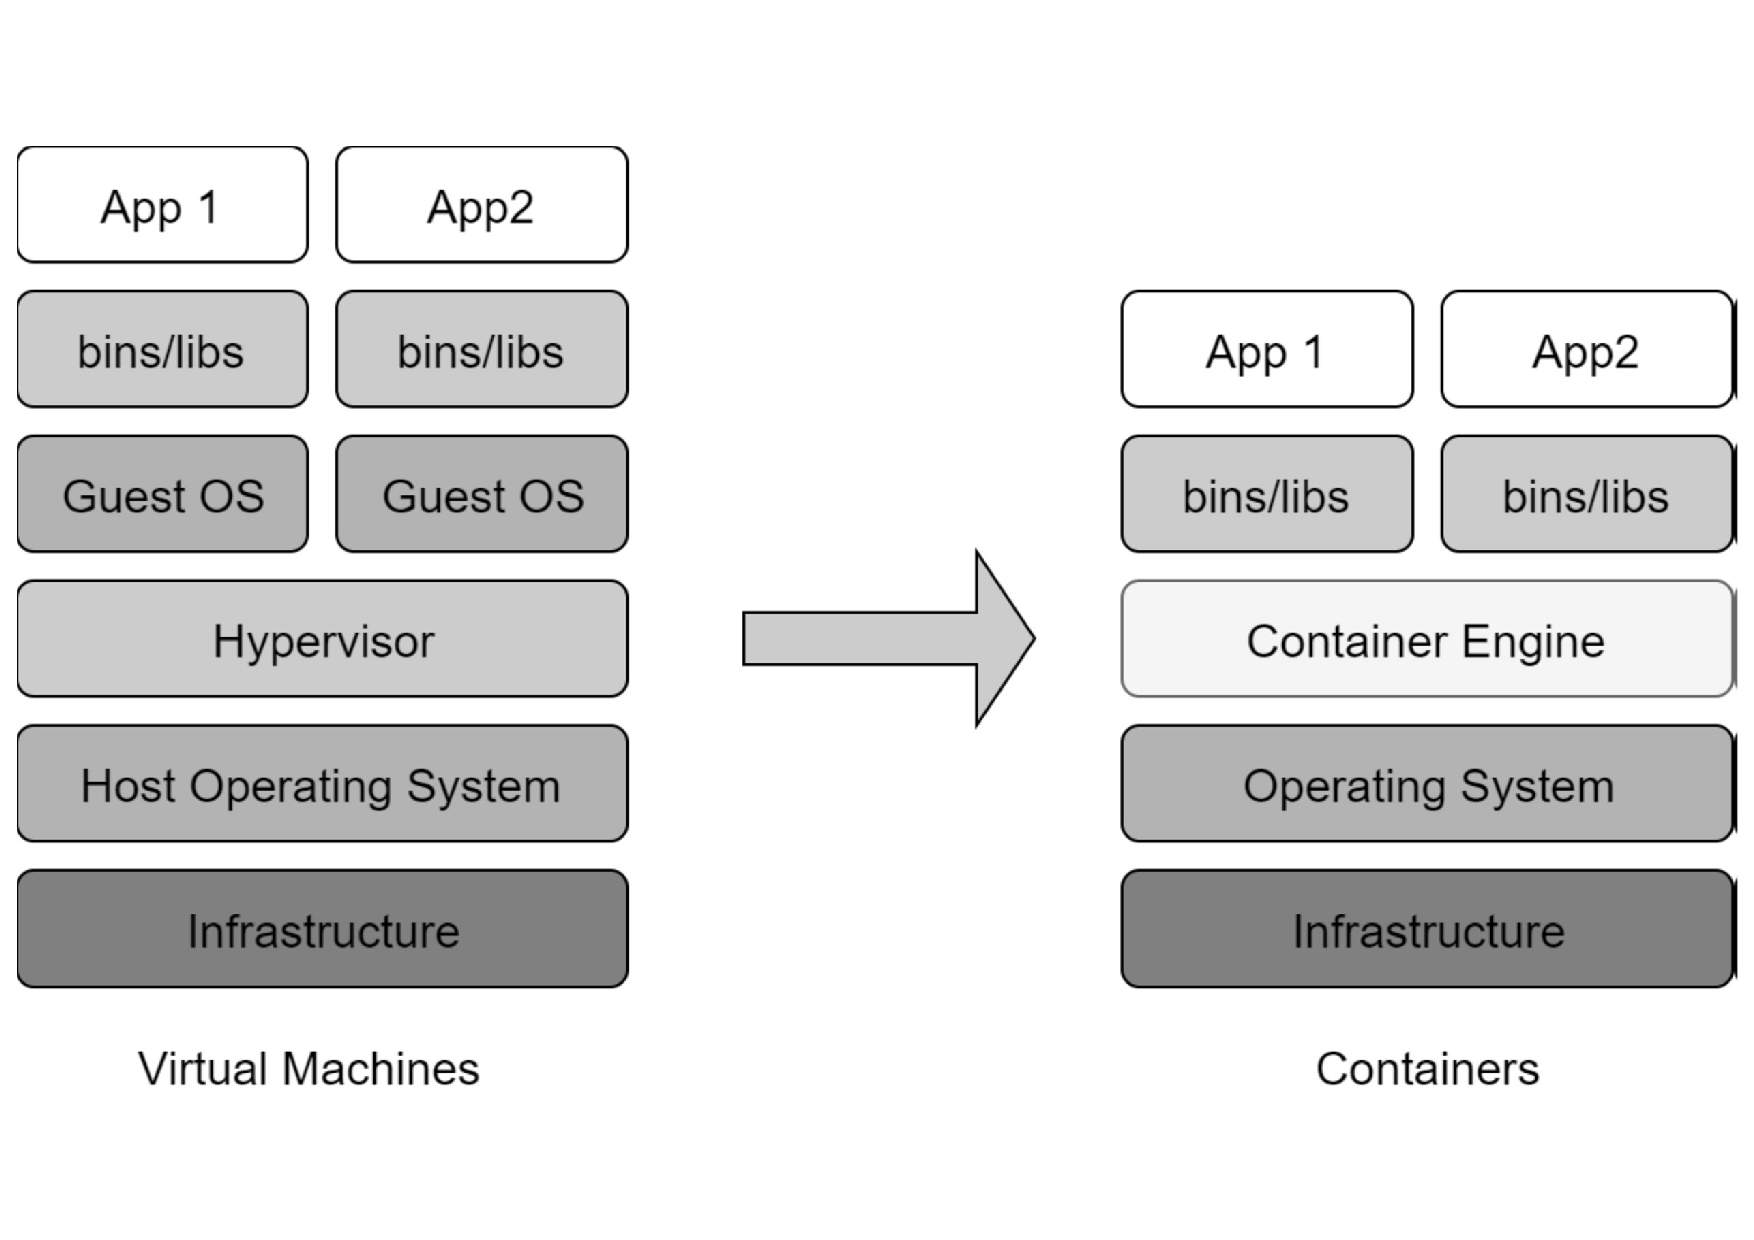
\includegraphics[width=\columnwidth]{Images/vm_vs_container.pdf}  
%	\caption[Architecture of virtual machines and containers]{The difference in  architecture between virtual machines and containers.}
%	\label{fig:vmVsContainer}
%\end{figure}

%Containerization is a OS-level virtualization technique that allows deploying and executing distributed applications without the need of launching an entire VM for each of the applications (\myFig{fig:vmVsContainer}). These multiple isolated systems are called containers. They are executed on top of a single host controller and access a single kernel.Since containers share the same OS kernel of the host, they can be a lot more efficient than a VM, that instead needs a separate instance of the OS. Containers own all the different components that are needed in order to execute the desired software, such as files, environment variables and libraries. The host OS controls the access of the container to the physical resources, such as CPU and memory, in order to prevent a single container from occupying the entire resources offered by the host.

%The main advantages of containerization come from efficiency in terms of memory, CPU and storage, when compared to traditional hardware virtualization. Since containers do not have the same overhead of VM, in particular we do not need different instances of the OS, it is possible to support more containers in the same infrastructure. Containerization offers better performances since there is a single OS that takes care of all the hardware calls. A particular point of interest for the container is the fact that they can be create much faster than the instances that are based on an hypervisor, this allows to have a more agile environment and allows the creation of new approaches, such as the microservices and continuous integration and delivery ones. 

%Potential disadvantages of containerization might be the absence of isolation from the host OS. Since containers share the same host OS, a potential security threat might easily gain access to the entire system. This did not happen when using virtualization based on an hypervisor, since in this case the only compromised component would be the VM. In order to circumvent this problem, a solution might be creating containers inside an OS that is run from a VM, this prevents the security breach at container level from letting the attacker gain access to the OS of the physical host. Another little disadvantage of containerization is that containers must execute the same OS as base OS, meanwhile instances based on an hypervisor are allowed to execute different OSs. Because of this, a container that is running on a Linux host, can neither execute an instance of Windows OS nor a Windows designed application.

%Containerization has gained more and more relevance thanks to the diffusion of the open source software Docker, that has developed a way to give more portability to the containers, allowing them to be moved from different systems that share the same kind of host OS without the need for changing lines of code. In particular, with Docker container there are no environment variables that must be set on the guest OS or library dependencies that need to be managed.


%\subsection{Docker}\label{sec:docker}
%Docker is an open source project that automatizes the deployment of applications inside software containers, giving a further abstraction thanks to OS level virtualization provided by Linux OS. Docker uses isolation functionalities provided by Linux kernel, such as cgroups and namespaces [8] in order to allow the coexistence of independent containers on the same Linux instance, avoiding the installation and maintenance of a VM.

%Linux kernel namespaces isolate what the application ca see of the operating environment, including process tree, network, user ids and mounted file system. Cgroups instead provide resource isolation, including CPU, memory, I/O devices and network.

%Docker implements a high level API in order to manage containers that execute in isolated environments. Since it uses Linux kernel functionalities, a Docker container, compared to a VM, does not includes a separated OS. Instead, it uses the kernel functionalities and exploits resource isolation and separated namespace in order to separate what each application can see of the underlying OS. Docker can access Linux kernel virtualization functionalities using different ways, for example directly using libcontainer or indirectly using libvirt, Linux Containers (LXC) or systemd-nspawn (\myFig{fig:docker}). 

%Using containers, resources can be isolated, services can be limited and processes can be started in a way that each of them has a private perspective of the OS, with their own identifier, file system and network interface. More container can share the same kernel, but each of them can be forced to use a different amount of resources such as CPU, memory and I/O. 

%By using Docker we can create and manage container in a way that simplifies the creation of distributed systems, allowing different applications and processes to work in an autonomous way on the same physical machine or on different virtual machines. This allows us to deploy new nodes only when necessary, in order to follow an evolution style that is similar to the platform as a service one.
%\begin{figure}
%	\centering
%	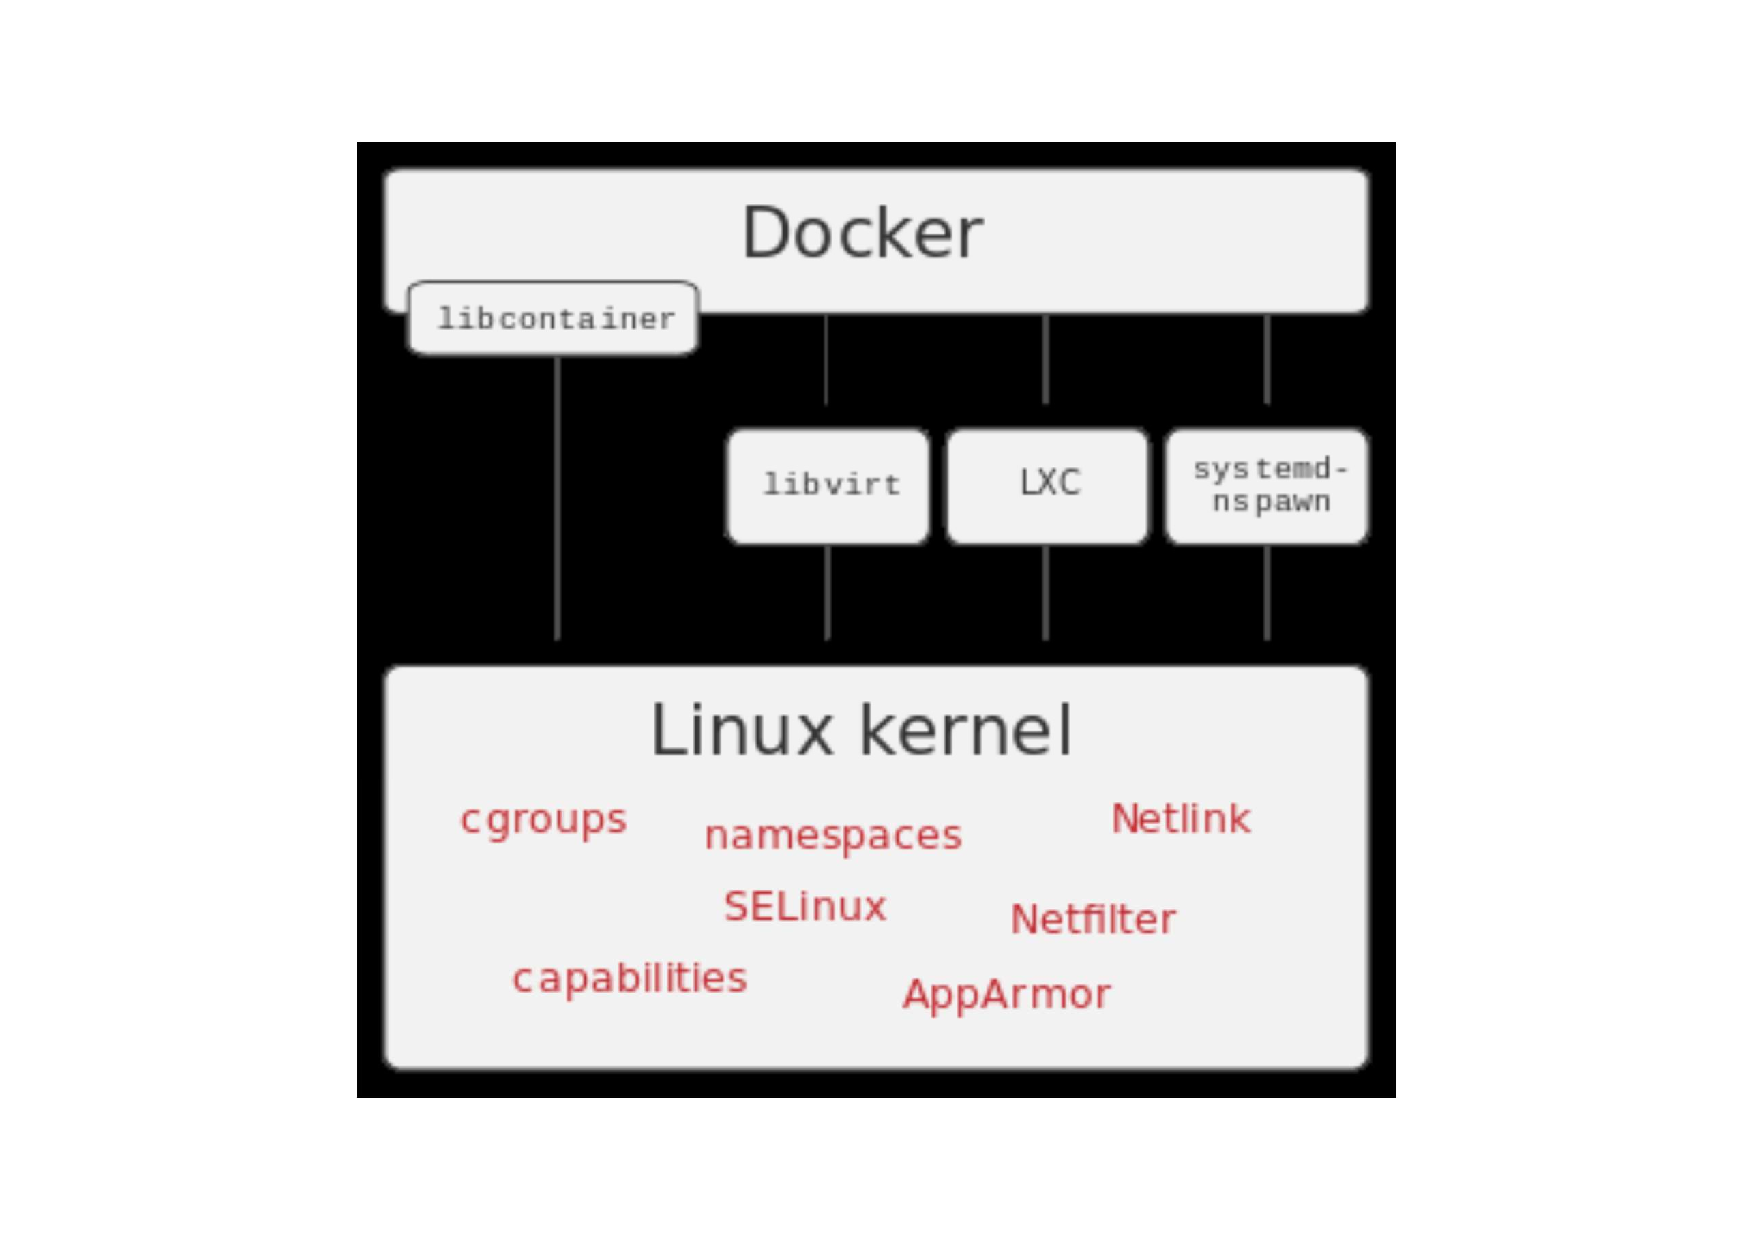
\includegraphics[width=\columnwidth]{Images/docker.pdf}  
%	\caption[Docker Interfaces]{Docker can use different interfaces in order to access Linux %kernel virtualization functionalities.}
%	\label{fig:docker}
%\end{figure}

\section{Symbolic Execution}
In computer science, the term symbolic execution refers to a software program analysis technique used to determine which data inputs cause the execution of each part of a program.

In this section we present an overview of \textit{symbolic execution}, taken primarily from a research work of Baldoni et al~\cite{Baldoni:2018:SSE:3212709.3182657}.

 It was introduced in the mid '70s %~\cite{K-ICRS75,SELECT-ICRS75,K-CACM76,H-TSE77} 
 mainly to test whether a software program could violate certain properties, e.g. that no divisions by zero are performed, no \texttt{null} pointers get dereferenced, no access to protected data can happen by unathorized users, etc. In general, it's not possible to decide every possible program property by means of automated checks, for example we cannot predict the target of an indirect jump. %, as it depends on values that are known at runtime. 
In practice, approximate and heuristic-based analyses are used in many cases.%, even in the field of mission-critical and security applications.

Software testing is performed to check that certain program properties hold for any possible usage scenario. A viable approach would be to test the program using a wide range of different, possibly random inputs. As the problem may occur only for very specific input values, we need to automate the exploration of the domain of the possible input data. 

With symbolic execution many possible execution paths are explored in parallel, without necessarily requiring concrete inputs. The idea is to replace the fully specified input data with symbols, that are their abstract representation, devolving to constraint solvers the construction of actual instances that would cause property violations. 

The symbolic execution intepreter walks through all the steps of the program, associating symbolic values to inputs rather than obtaining their actual values, building  expressions in terms of those symbols and program variables, and constraints in terms of the symbols corresponding to the possible outcomes of each conditional branch. 

When a program is run with a specific set of input data (a concrete execution), a single control flow path is explored. Hence, concrete executions can only under-approximate the analysis of the property of interest. With symbolic execution, multiple paths that a program could take under different inputs can be simultaneously explored. This means that a sound analyses can be done, giving stronger guarantees about the checked property%~\cite{Baldoni:2018:SSE:3212709.3182657}
. When a program runs with {\em symbolic} -- rather than concrete -- input values, the execution is performed by a {\em symbolic execution engine}, which builds and updates a structure to hold (i) a first-order Boolean {\em formula} describing the conditions satisfied by all the traversed branches along that path, and (ii) a {\em symbolic memory store} mapping variables to symbolic expressions or values, for each path traversed by the control flow. Execution of a branch updates the formula, while assignments update the symbolic store. Finally, a {\em model checker}, commonly based on a {\em satisfiability modulo theories} (SMT) solver%~\cite{BKM14}
, is used to verify if the property is violated somewhere along each explored path and if the path itself is concretely feasible, i.e., if any assignment of concrete values to the program's symbolic arguments exists that satisfies its formula%~\cite{Baldoni:2018:SSE:3212709.3182657}
.

%Symbolic execution techniques have been emphasized to a wide audience following the DARPA announcement in 2013 at the Cyber Grand Challenge, a two-year competition pursuing the creation of automatic systems for vulnerability detection, exploitation, and patching in near real-time~\cite{ANGR-SSP16}.
%More important, symbolic execution based engines have been running 24/7 in the testing process of many Microsoft applications since 2008, discovering nearly 30\% of all the flaws discovered by file fuzz testing during the development of Windows 7, which other program analyses and blackbox testing techniques missed~\cite{SAGE-QUEUE12}.

\paragraph{Example}


\label{symbolic-execution-example}
\begin{figure}[t]
	\begin{center}
		\begin{tabular}{c}
			\hspace{-4.5cm}
			\begin{lstlisting}[basicstyle=\ttfamily\scriptsize]
			1.  void foo(int a, int b) {
			2.     int x = 1, y = 0;
			3.     if (a != 0) {
			4.        y = 3+x;
			5.        if (b == 0)
			6.           x = 2*(a+b);
			7.     }
			8.     assert(x-y != 0);
			9.  }
			\end{lstlisting}
		\end{tabular}
	\end{center}
	\vspace{-2mm}
	\caption{Example: which values of \texttt{a} and \texttt{b} make the \texttt{assert} fail?}
	\label{fig:example-1}
	\vspace{-1.5mm}
\end{figure}

With reference to the C code in \MyFig{fig:example-1}, let's say we want to discover which of the $2^{32}$ possible \texttt{4-byte} inputs make the \texttt{assert} at line 8 of function \texttt{foo} fail. If we address the problem by running concretely the function \texttt{foo} on randomly generated inputs, we will unlikely pick up exactly the assert-failing inputs. Symbolic execution go beyond this limitation by reasoning on {\em classes of inputs}, rather than single input values, thanks to the evaluation of the code using symbols for its inputs, instead of concrete values,  

Going further into details, a symbol $\alpha_i$ is associated to each value that cannot be resolved by a static analysis of the code, e.g. an actual parameter of a function or data read from an input stream. A state $(stmt,~\sigma,~\pi)$ is kept by the symbolic execution engine, where:

\begin{itemize}
	\item $stmt$ is the next statement to evaluate. At this time, we assume that $stmt$ can be an assignment, a conditional branch, or a jump.
	
	\item $\sigma$ is a {\em symbolic store} that associates program variables with concrete values of expressions or symbolic values $\alpha_i$.
	
	\item $\pi$ identifies the {\em path constraints}, i.e., it is a formula expressing a set of assumptions on the symbols $\alpha_i$ as a result of branches taken in the execution to reach $stmt$. At the start of the analysis, $\pi=true$.
\end{itemize}

\noindent Depending on $stmt$, the symbolic engine changes the state as follows:

\begin{itemize}
	\item The evaluation of an assignment $x=e$ updates the symbolic store $\sigma$ by associating $x$ with a new symbolic expression $e_s$. We express this association with $x\mapsto e_s$, where $e_s$ is obtained by evaluating $e$ in the context of the current execution state and  can be any expression involving unary or binary operators over symbols and concrete values.
	\item The evaluation of a conditional branch ${\texttt if}~e~{\texttt then}~s_{true}~{\texttt else}~s_{false}$ affects the path constraints $\pi$. The symbolic execution is forked by creating two execution states with path constraints $\pi_{true}$ and $\pi_{false}$, respectively, which correspond to the two branches: $\pi_{true}=\pi \wedge e_s$ and $\pi_{false}=\pi \wedge \neg e_s$, where $e_s$ is a symbolic expression obtained by evaluating $e$. 
	Symbolic execution independently proceeds on both states.
	\item The evaluation of a jump {\texttt goto} $s$ updates the execution state by advancing the symbolic execution to statement $s$. 
\end{itemize}

\begin{figure}[t]
	%\centering
	\hspace{-3cm}
	%
	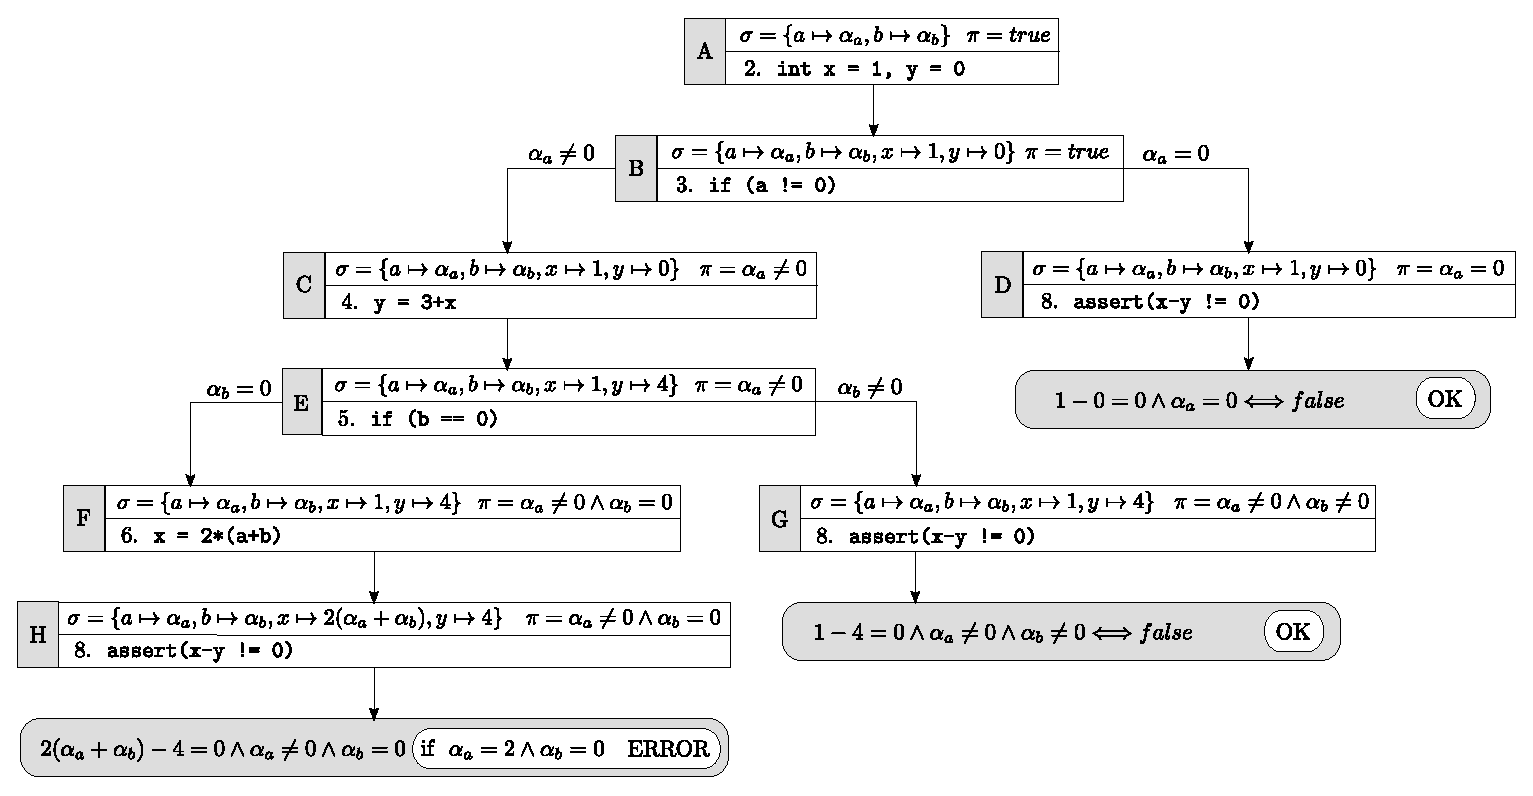
\includegraphics[width=1.5\columnwidth]{images/execution-tree.eps} 
	%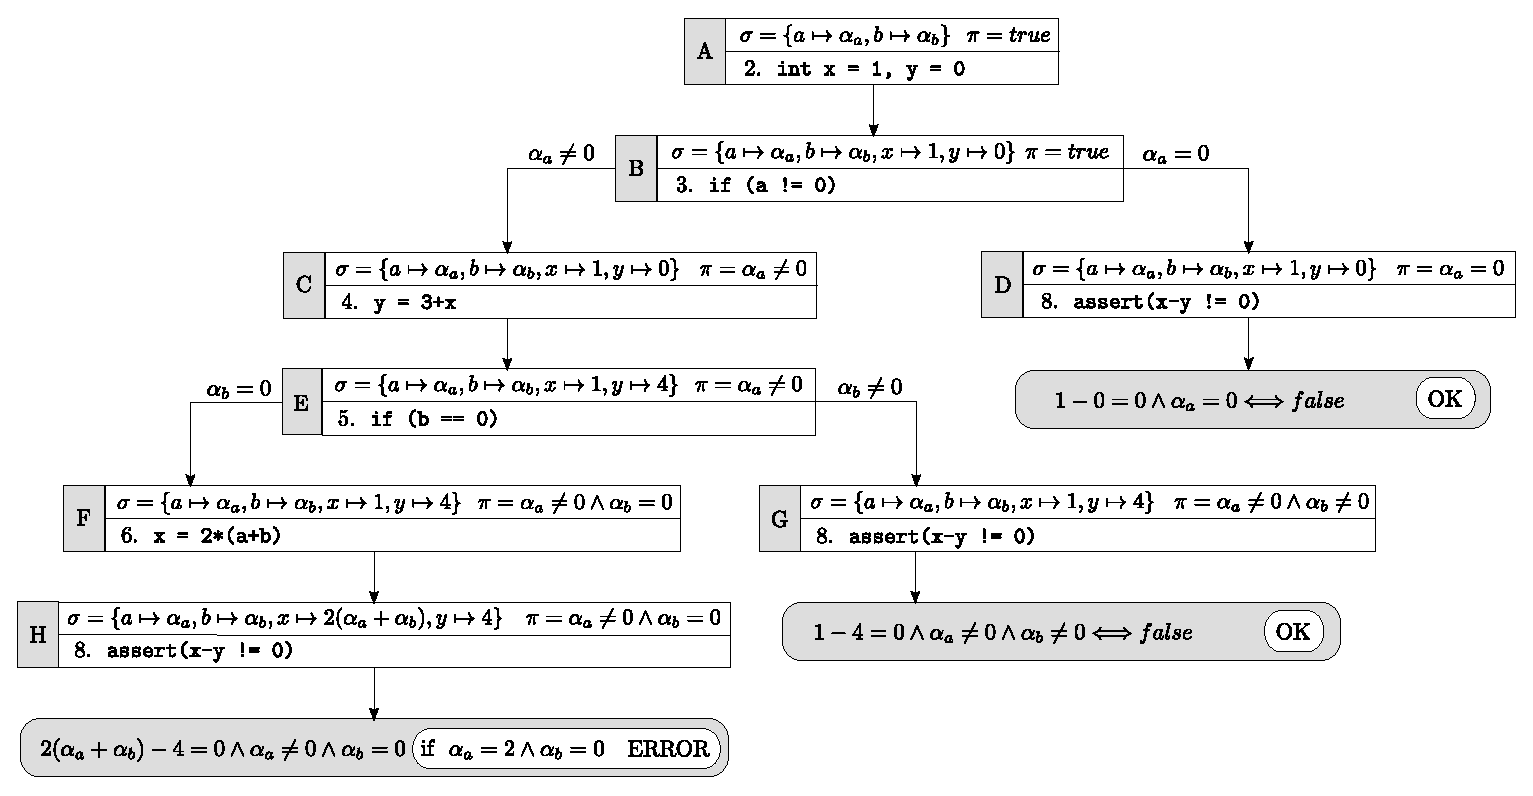
\includegraphics[width=18cm]{images/execution-tree.eps} 
	\caption{Symbolic execution tree of function {\texttt foo} given in \MyFig{fig:example-1}. Each execution state, labeled with an upper case letter, shows the statement to be executed, the symbolic store $\sigma$, and the path constraints $\pi$. Leaves are evaluated against the condition in the {\texttt assert} statement. Image courtesy of Association for Computing Machinery~\cite{Baldoni:2018:SSE:3212709.3182657}.}
	%For the sake of presentation the conjunction of constraints is shown as a list of constraints. }
	\label{fig:example-symbolic-execution}
	\vspace{-1mm}
\end{figure}

\noindent \MyFig{fig:example-symbolic-execution} shows a symbolic execution of function {\texttt foo}, that can be adequately represented as a tree. In the initial state (execution state $A$) the path constraints are {\texttt true} and input arguments {\texttt a} and {\texttt b} are associated with symbolic values. 
After local variables initialization {\texttt x} and {\texttt y} at line 2, the symbolic store is updated by associating {\texttt x} and {\texttt y} with concrete values 1 and 0, respectively (execution state $B$). A conditional branch is met in line 3 and the execution is forked:according to which branch is taken, a different statement is evaluated and different assumptions are made on symbol $\alpha_a$ (execution states $C$ and $D$). In the branch corresponding to $\alpha_a\neq 0$, variable {\texttt y} is assigned to  ${\texttt x}+3$, obtaining $y\mapsto 4$ in state $E$ because $x\mapsto 1$ in state $C$. Arithmetic expression evaluation, generally, change only the symbolic values.
When the {\texttt assert} at line 8 is reached by fully expanding every execution state  on all branches, we can check which input values for parameters {\texttt a} and {\texttt b} can make the {\texttt assert} fail. By analyzing execution states $\{D,G,H\}$, we can conclude that only $H$ can make {\texttt x-y = 0} true. The path constraints for $H$ at this point implicitly define the set of inputs that are unsafe for \texttt{foo}. 
In particular, any input values such that:
\[ 2(\alpha_a+\alpha_b)-4 = 0 \wedge \alpha_a \neq 0 \wedge \alpha_b = 0 \]
will make {\texttt assert} fail. An instance of unsafe input parameters can be eventually determined by invoking an {\em SMT solver}%~\cite{BKM14}
 to solve the path constraints, which in this example would yield $a = 2$ and $b = 0$.

The example shown represents a case where symbolic execution can derive {\em all} the inputs that make the {\texttt assert} fail, by exploring all the possible execution states. With regards to the underpinning theory, exhaustive symbolic execution represents a {\em sound} and {\em complete} methodology for any decidable analysis~\cite{Baldoni:2018:SSE:3212709.3182657}. Soundness (no false negatives) means that all possible unsafe inputs are guaranteed to be found, while completeness (no false positives) means that  input values deemed unsafe are actually unsafe. Exhaustive symbolic execution cannot be easily scalable beyond small-sized applications. In many practical cases, a trade-off between soundness and performance approach is used.
